% ******************************* PhD Thesis Template **************************
% Please have a look at the README.md file for info on how to use the template

\documentclass[a4paper,customfont,custombib,custommargin,print]{Classes/PhDThesisPSnPDF}

% ******************************************************************************
% ******************************* Class Options ********************************
% *********************** See README for more details **************************
% ******************************************************************************

% `a4paper'(The University of Cambridge PhD thesis guidelines recommends a page
% size a4 - default option) or `a5paper': A5 Paper size is also allowed as per
% the Cambridge University Engineering Deparment guidelines for PhD thesis
%
% `11pt' or `12pt'(default): Font Size 10pt is NOT recommended by the University
% guidelines
%
% `oneside' or `twoside'(default): Printing double side (twoside) or single
% side.
%
% `print': Use `print' for print version with appropriate margins and page
% layout. Leaving the options field blank will activate Online version.
%
% `index': For index at the end of the thesis
%
% `draftclassic': For draft mode without loading any images (same as draft in book)
%
% `draft': Special draft mode with line numbers, images, and water mark with
% timestamp and custom text. Position of the text can also be modified.
%
% `abstract': To generate only the title page and abstract page with
% dissertation title and name, to submit to the Student Registry
%
% `chapter`: This option enables only the specified chapter and it's references
%  Useful for review and corrections.
%
% ************************* Custom Page Margins ********************************
%
% `custommargin`: Use `custommargin' in options to activate custom page margins,
% which can be defined in the preamble.tex. Custom margin will override
% print/online margin setup.
%
% *********************** Choosing the Fonts in Class Options ******************
%
% `times' : Times font with math support. (The Cambridge University guidelines
% recommend using times)
%
% `fourier': Utopia Font with Fourier Math font (Font has to be installed)
%            It's a free font.
%
% `customfont': Use `customfont' option in the document class and load the
% package in the preamble.tex
%
% default or leave empty: `Latin Modern' font will be loaded.
%
% ********************** Choosing the Bibliography style ***********************
%
% `authoryear': For author-year citation eg., Krishna (2013)
%
% `numbered': (Default Option) For numbered and sorted citation e.g., [1,5,2]
%
% `custombib': Define your own bibliography style in the `preamble.tex' file.
%              `\RequirePackage[square, sort, numbers, authoryear]{natbib}'.
%              This can be also used to load biblatex instead of natbib
%              (See Preamble)
%
% **************************** Choosing the Page Style *************************
%
% `default (leave empty)': For Page Numbers in Header (Left Even, Right Odd) and
% Chapter Name in Header (Right Even) and Section Name (Left Odd). Blank Footer.
%
% `PageStyleI': Chapter Name next & Page Number on Even Side (Left Even).
% Section Name & Page Number in Header on Odd Side (Right Odd). Footer is empty.
%
% `PageStyleII': Chapter Name on Even Side (Left Even) in Header. Section Number
% and Section Name in Header on Odd Side (Right Odd). Page numbering in footer


% ********************************** Preamble **********************************
% Preamble: Contains packages and user-defined commands and settings
% ******************************************************************************
% ****************************** Custom Margin *********************************

% Add `custommargin' in the document class options to use this section
% Set {innerside margin / outerside margin / topmargin / bottom margin}  and
% other page dimensions
\ifsetCustomMargin
  \RequirePackage[left=37mm,right=30mm,top=35mm,bottom=30mm]{geometry}
  \setFancyHdr % To apply fancy header after geometry package is loaded
\fi

% Add spaces between paragraphs
%\setlength{\parskip}{0.5em}
% Ragged bottom avoids extra whitespaces between paragraphs
\raggedbottom
% To remove the excess top spacing for enumeration, list and description
%\usepackage{enumitem}
%\setlist[enumerate,itemize,description]{topsep=0em}

% *****************************************************************************
% ******************* Fonts (like different typewriter fonts etc.)*************

% Add `customfont' in the document class option to use this section

\ifsetCustomFont
  % Set your custom font here and use `customfont' in options. Leave empty to
  % load computer modern font (default LaTeX font).

  \renewcommand{\familydefault}{\sfdefault}
  \RequirePackage[scaled=1]{helvet}
  
  %for math
  \usepackage[helvet]{sfmath}  
  %\usepackage{sansmathfonts}   
  %\usepackage{sansmath}
  %\everymath={\sf}
   
  %for dedication
  \usepackage{miama}
   
  
  % For use with XeLaTeX
  %  \setmainfont[
  %    Path              = ./libertine/opentype/,
  %    Extension         = .otf,
  %    UprightFont = LinLibertine_R,
  %    BoldFont = LinLibertine_RZ, % Linux Libertine O Regular Semibold
  %    ItalicFont = LinLibertine_RI,
  %    BoldItalicFont = LinLibertine_RZI, % Linux Libertine O Regular Semibold Italic
  %  ]
  %  {libertine}
  %  % load font from system font
  %  \newfontfamily\libertinesystemfont{Linux Libertine O}
\fi

% *****************************************************************************
% **************************** Custom Packages ********************************
\usepackage{lipsum} %generate paragraphs of dummy lorem ipsum text

% ************************* Algorithms and Pseudocode **************************

%\usepackage{algpseudocode}

% ********************Captions and Hyperreferencing / URL **********************

% Captions: This makes captions of figures use a boldfaced small font.
%\RequirePackage[small,bf]{caption}

\RequirePackage[labelsep=space,tableposition=top]{caption}
\renewcommand{\figurename}{Fig.} %to support older versions of captions.sty
\renewcommand{\figureautorefname}{Fig.}


% *************************** Graphics and figures *****************************

%\usepackage{rotating}
%\usepackage{wrapfig}

% Uncomment the following two lines to force Latex to place the figure.
% Use [H] when including graphics. Note 'H' instead of 'h'
%\usepackage{float}
%\restylefloat{figure}

% Subcaption package is also available in the sty folder you can use that by
% uncommenting the following line
% This is for people stuck with older versions of texlive
%\usepackage{sty/caption/subcaption}
\usepackage{subcaption}

% ********************************** Tables ************************************
\usepackage{booktabs} % For professional looking tables
\usepackage{multirow}

%\usepackage{multicol}
%\usepackage{longtable}
%\usepackage{tabularx}


% *********************************** SI Units *********************************
\usepackage{siunitx} % use this package module for SI units


% ******************************* Line Spacing *********************************

% Choose linespacing as appropriate. Default is one-half line spacing as per the
% University guidelines

% \doublespacing
% \onehalfspacing
% \singlespacing


% ************************ Formatting / Footnote *******************************

% Don't break enumeration (etc.) across pages in an ugly manner (default 10000)
%\clubpenalty=500
%\widowpenalty=500

%\usepackage[perpage]{footmisc} %Range of footnote options


% *****************************************************************************
% *************************** Bibliography  and References ********************

%\usepackage{cleveref} %Referencing without need to explicitly state fig /table

% Add `custombib' in the document class option to use this section
\ifuseCustomBib
   %\RequirePackage[square, sort, numbers, authoryear]{natbib} % CustomBib

% If you would like to use biblatex for your reference management, as opposed to the default `natbibpackage` pass the option `custombib` in the document class. Comment out the previous line to make sure you don't load the natbib package. Uncomment the following lines and specify the location of references.bib file

\RequirePackage[backend=biber, backref, style=numeric-comp, citestyle=numeric, sorting=none, natbib=true,isbn=false,url=false,eprint=false]{biblatex}
\bibliography{References/references} %Location of references.bib only for biblatex

\fi

% changes the default name `Bibliography` -> `References'
\renewcommand{\bibname}{References}


% ******************************************************************************
% ************************* User Defined Commands ******************************
% ******************************************************************************

% *********** To change the name of Table of Contents / LOF and LOT ************

%\renewcommand{\contentsname}{My Table of Contents}
%\renewcommand{\listfigurename}{My List of Figures}
%\renewcommand{\listtablename}{My List of Tables}


% ********************** TOC depth and numbering depth *************************

\setcounter{secnumdepth}{2}
\setcounter{tocdepth}{2}


% ******************************* Nomenclature *********************************

% To change the name of the Nomenclature section, uncomment the following line

%\renewcommand{\nomname}{Symbols}


% ********************************* Appendix ***********************************

% The default value of both \appendixtocname and \appendixpagename is `Appendices'. These names can all be changed via:

%\renewcommand{\appendixtocname}{List of appendices}
%\renewcommand{\appendixname}{Appndx}

% *********************** Configure Draft Mode **********************************

% Uncomment to disable figures in `draft'
%\setkeys{Gin}{draft=true}  % set draft to false to enable figures in `draft'

% These options are active only during the draft mode
% Default text is "Draft"
%\SetDraftText{DRAFT}

% Default Watermark location is top. Location (top/bottom)
%\SetDraftWMPosition{bottom}

% Draft Version - default is v1.0
%\SetDraftVersion{v1.1}

% Draft Text grayscale value (should be between 0-black and 1-white)
% Default value is 0.75
%\SetDraftGrayScale{0.8}


% ******************************** Todo Notes **********************************
%% Uncomment the following lines to have todonotes.

\ifsetDraft
	\usepackage[colorinlistoftodos]{todonotes}
	\newcommand{\mynote}[1]{\todo[author=erpan,size=\small,inline,color=green!40]{#1}}
\else
	\newcommand{\mynote}[1]{}
	\newcommand{\listoftodos}{}
\fi

% Example todo: \mynote{Hey! I have a note}


% ************************ Thesis Information & Meta-data **********************
% Thesis title and author information, refernce file for biblatex
% ************************ Thesis Information & Meta-data **********************
%% The title of the thesis
\title{First-principles Studies of Novel Two-dimensional Materials and Their Physical Properties}
%\texorpdfstring is used for PDF metadata. Bookmark could not display correct titles
%Usage:
%\texorpdfstring{LaTeX_Version}{PDF Version (non-latex)} eg.,
%\texorpdfstring{$sigma$}{sigma}

%% Subtitle (Optional)
%\subtitle{}

%% The full name of the author
\author{Yierpan Aierken}

%% Department (eg. Department of Engineering, Maths, Physics)
\dept{Department of Physics}

%% University and Crest
\university{University of Antwerp}
% Crest minimum should be 30mm.
\crest{
\includegraphics[width=0.4\textwidth]{Figs/UA_HOR_NED_CMYK.eps}}
%% Use this crest, if you are using the college crest
%% Crest long miminum should be 65mm
%\crest{
\includegraphics[width=0.45\textwidth]{University_Crest_Long}}

%% College shield [optional] 
% Crest minimum should be 30mm.
\collegeshield{
\includegraphics[width=0.2\textwidth]{Nano_logo.png}}


%% Supervisor (optional)
%% for multiple supervisors, append each supervisor with the \newline command
\supervisor{Prof. François M. Peeters}% \newline
%Prof. C.D. Supervisor}

%% Supervisor Role (optional) - Supervisor (default) or advisor
% \supervisorrole{\textbf{Supervisors: }}
%% if no title is desired:
% \supervisorrole{}

%% Supervisor line width: required to align supervisors
\supervisorlinewidth{0.38\textwidth}

%% Advisor (optional)
%% for multiple advisors, append each advisor with the \newline command
\advisor{Dr. Ortwin Leenaerts \newline
Dr. Deniz Çakır}
     
%% Advisor Role (optional) - Advisor (default) or leave empty
% \advisorrole{Advisors: }
%% if no title is required
% \advisorrole{}

%% Advisor line width: required to align supervisors
\advisorlinewidth{0.33\textwidth}


%% You can redefine the submission text:
% Default as per the University guidelines:
% ``This dissertation is submitted for the degree of''
%\renewcommand{\submissiontext}{change the default text here if needed}

%% Full title of the Degree
\degreetitle{Doctor of Philosophy}

%% College affiliation (optional)
\college{Antwerp, Belgium}

%% Submission date
% Default is set as {\monthname[\the\month]\space\the\year}
%\degreedate{September 2014} 

%% Meta information
\subject{LaTeX} \keywords{{LaTeX} {PhD Thesis} {Physics} {University of
Antwerp}}


% ***************************** Abstract Separate ******************************
% To printout only the titlepage and the abstract with the PhD title and the
% author name for submission to the Student Registry, use the `abstract' option in
% the document class.

\ifdefineAbstract
 \pagestyle{empty}
 \includeonly{Declaration/declaration, Abstract/abstract}
\fi

% ***************************** Chapter Mode ***********************************
% The chapter mode allows user to only print particular chapters with references
% Title, Contents, Frontmatter are disabled by default
% Useful option to review a particular chapter or to send it to supervisior.
% To use choose `chapter' option in the document class

\ifdefineChapter
 \includeonly{Chapter1/chapter1}
\fi

% ******************************** Front Matter ********************************
\begin{document}

\frontmatter

\maketitle

\clearpage

%start a new page
\thispagestyle{empty}

\begin{list}{}{\leftmargin=0cm}

\item \textbf{Members of the Jury:}

\item \textbf{Chairman} \\
Prof. Dr. Dirk Lamoen, Universiteit Antwerpen, Belgium \\

\item \textbf{Supervisor} \\
Prof. Dr. Fran\c{c}ois Peeters, Universiteit Antwerpen, Belgium\\

\item \textbf{Members} \\
Prof. Dr. Sandra Van Aert, Universiteit Antwerpen, Belgium \\
Prof. Dr. Michel Houssa, The Katholieke Universiteit Leuven, Belgium \\
\end{list}

\vspace{0.7cm}

\begin{list}{}{\leftmargin=0cm}
            \item \textbf{Contact Information:}
            \item    Yierpan Aierken \\
            G.U. 212 \\
            Groenenborgerlaan 171 \\
            2020 Antwerpen \\
            Belgium \\
            yierpan.aierken@uantwerpen.be
\end{list}
\vspace{0.7cm}

\begin{list}{}{\leftmargin=0cm}
\item \textbf{Reseach units:}
\begin{flushleft}

\includegraphics[width =0.6\textwidth]{Figs/research_units.eps}
\end{flushleft}
\end{list}

\vfill
\begin{list}{}{\leftmargin=0cm}
\item \textbf{Funding agency:}
\begin{flushleft}

\includegraphics[width =0.6\textwidth]{Figs/FWO.eps}
\end{flushleft}
\end{list}
% ******************************* Thesis Dedidcation ********************************

\begin{dedication} 




\begin{LARGE}
{\fmmfamily I would like to dedicate this thesis \\
to my loving parents Arkin and Perwin, \\
to my beloved wife Adila,  \\
to my cherished sons Efran and Wildan.}
\end{LARGE}




\end{dedication}


%% ******************************* Thesis Declaration ***************************

\begin{declaration}

I hereby declare that except where specific reference is made to the work of others, the contents of this dissertation are original and have not been submitted in whole or in part for consideration for any other degree or qualification in this, or any other university. This dissertation is my own work and contains nothing which is the outcome of work done in collaboration with others, except as specified in the text and Acknowledgements. This dissertation contains fewer than 65,000 words including bibliography, footnotes, tables and equations and has fewer than 100 figures.

% Author and date will be inserted automatically from thesis.tex \author \degreedate

\end{declaration}


% ************************** Thesis Acknowledgements **************************

\begin{acknowledgements}      


And I would like to acknowledge ...


\end{acknowledgements}

% ************************** Thesis Abstract *****************************
% Use `abstract' as an option in the document class to print only the titlepage and the abstract.
\begin{abstract}
This is where you write your abstract ...
\end{abstract}

\nomenclature{2D}{two-dimensional}
\nomenclature{3D}{three-dimensional}
\nomenclature{QHA}{quasi-harmonic approximation}
\nomenclature{PAW}{projected-augemeted wave}
\nomenclature{TEC}{thermal expansion coefficients}
\nomenclature{TMDs}{Transition metal dichalcogenides}
\nomenclature{VBM}{valence band maximum}
\nomenclature{CBM}{conduction band minimum}
\nomenclature{vdW}{van der Waals}
\nomenclature{cNEB}{climbing-image nudge elastic band}
\nomenclature{AEMHs}{alkaline earth metal hydroxides}
\nomenclature{DOS}{density of states}
\nomenclature{pDOS}{partial density of states}
\nomenclature{DFPT}{density functional perturbation theory}
\nomenclature{DPC}{deformation potential constant}
\nomenclature{NEGF}{non-equilibrium Green's functions}
\nomenclature{EP}{electrostatic potential}
\nomenclature{PNT}{phosphorene nanotubes}
\nomenclature{PES}{potential energy surface}
\nomenclature{GGA}{generalized gradient approximation}
\nomenclature{LDA}{local density approximation}
\nomenclature{HF}{Hartree-Fock}
\nomenclature{HSE}{Heyd-Scuseria-Ernzerhof}
\nomenclature{MAE}{mean absolute error}
\nomenclature{VASP}{Vienna $Ab$ $initio$ Simulation Package}
\nomenclature{SOC}{spin-orbit coupling}
\nomenclature{CVD}{Chemical vapor deposition}

% *********************** Adding TOC and List of Figures ***********************

\tableofcontents

\listoffigures

\listoftables

% \printnomenclature[space] space can be set as 2em between symbol and description
%\printnomenclature[3em]

\printnomenclature

% ******************************** Main Matter *********************************
\mainmatter

%!TEX root = ../thesis.tex
%*******************************************************************************
%*********************************** First Chapter *****************************
%*******************************************************************************

\chapter{Introduction \label{chap:1}}  %Title of the First Chapter

\ifpdf
    \graphicspath{{Chapter1/Figs/Raster/}{Chapter1/Figs/PDF/}{Chapter1/Figs/}{Chapter1/Figs/Vector/}}
\else
    \graphicspath{{Chapter1/Figs/Vector/}{Chapter1/Figs/}}
\fi



A new field of research in material science and condensed matter physics was formed after the synthesis of graphene in 2004 \cite{Novoselov666,Novoselov26072005}. This field is named Two-dimensional (2D) material due to the fact that graphene is a single atomic-layer crystal. The synthesis itself together with the phenomenal properties of graphene has leaded to a Nobel Price in physics rewarded to A. K. Geim and K. S. Novoselov \cite{Geim2007}. Since then, the field is expanding with the involvement of researcher not only from young community, but also from experts who have been working on materials like graphite, fullerenes and carbon nanotubes which are strongly graphene related. In the last several years, researches focused on graphene and related topics increasing rapidly, see \autoref{fig:grpapers}. While a part of these effects have been making to explore more on the graphene itself and its applications, some other parts were put on discovering new 2D materials. It has been evidenced from graphene, same material having different dimensionality can have different properties. Therefore, many materials with hidden properties which will only manifest itself at other dimensions yet to be discovered. 


\begin{figure}[htbp!] 
\centering  
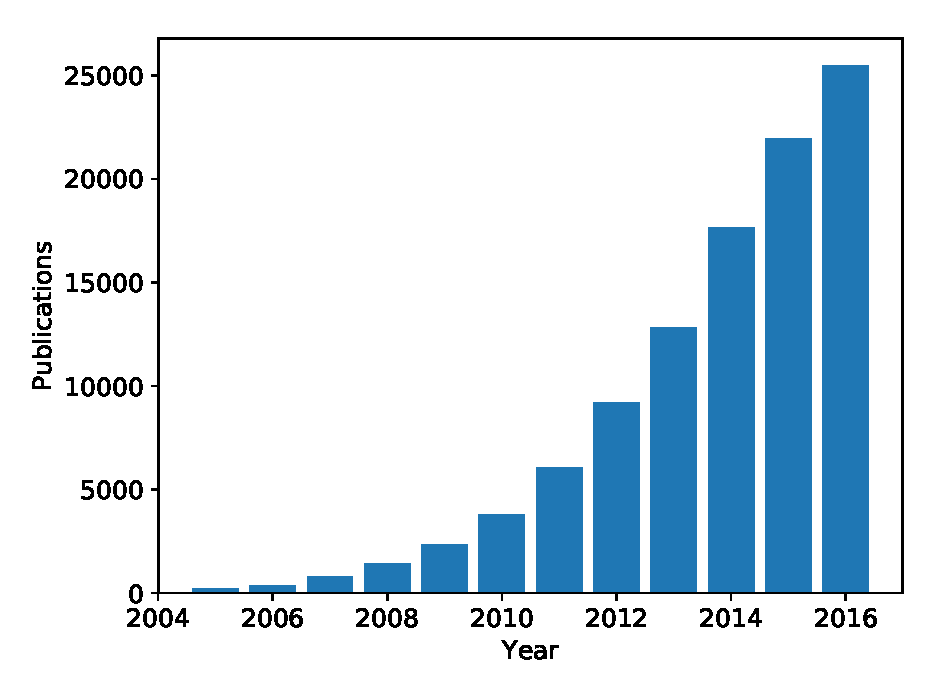
\includegraphics[width=0.7\textwidth]{graphene_papers.eps}
\caption[Graphene publications]{Graphene related publications during the last decade. Data source: ISI Web of Science. \protect\footnotemark }  
\label{fig:grpapers}
\end{figure} 

On the other hand, with the advent of powerful supercomputer facilities, calculations that seems impossible to finish in a reasonable time now has been made accessible. At the same time, given the accuracy of the calculations is the most crucial aspect of computational physics, especially when the results are related to the prediction the real properties of materials, researchers and programmers have been making important progress to make sure theories and its implementation are correct and the results they yield are within acceptable precision. Equipped with these tools, theoretical predictions on the structure and the properties of material have served well on discovering unexplored features. Moreover, detailed characterizations at atomic scale benefits the experimental results to make it more convincing, or even sometimes to explain the unexpected results.

\footnotetext{This result is obtained by searching for "graphene" in the topic field of Web of Science.}

Considering all mentioned, it is a sound approach to apply the state-of-the-art computational methods that accompanied with high-performance supercomputer facilities to investigate the physical properties of novel 2D materials. This thesis is a summary of several works which has accomplished during my PhD study and were initiated to this end. The thesis is organized as followed: For the rest of this chapter, I will first introduce graphene and some post-graphene materials that discovered right after graphene and, briefly, methods used to synthesis 2D materials. The following \autoref{chap:2} will present the computational methods, the theory behind and the implementations of them. In \autoref{chap:3}, I will discuss several general properties of 2D materials. The next two chapters will be the main results from my works. Starting from specific properties targeting at specific novel 2D materails in \autoref{chap:4}, and followed by modification of physical properties of 2D materials in \autoref{chap:5}. Conclusions for the thesis will be given in the last chapter.

\section{Graphene}

Graphene is composed of carbon (C) atoms arranged on a hexagonal lattice. Each C atoms bond to three neighbouring C atoms. Graphene is one single atomic layer of graphite, see \autoref{fig:gra_grap}. These layers in graphite are stacked on top of another through weak physical bonding, whereas within each layer C atoms are hold together by strong chemical bonding. As a result, it is possible to just isolate single layer from graphite without damaging the layer itself. 

\begin{figure}[htbp!] 
\centering  
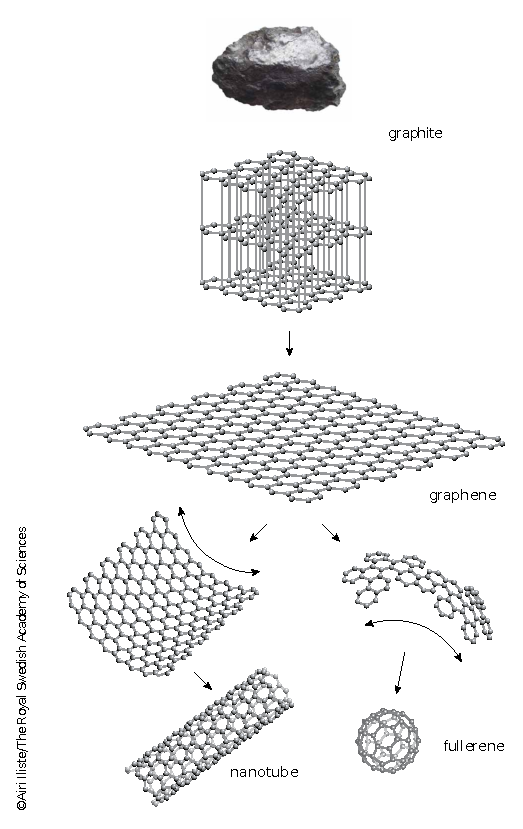
\includegraphics[width=0.7\textwidth]{gra_grap.eps}
\caption{Relation of graphite, graphene, fullerene and nanotube. Image source: the Nobel prize in physics 2010 \cite{gra_grap}. }  
\label{fig:gra_grap}
\end{figure} 


\subsection{History}

The story of graphene can be trace back to the discover of graphite around 1564 in England\cite{petroski1990pencil}. Ever since, people have been using the graphite, the tip of a pencil, for writing and drawing. The black trace left behind by pencil they are actually stacks of graphite and graphene, by chance even a single layer graphene can present.  Apart from being a part of a pencil, graphite certainly has been holding a important position in technology and industry due to its rich chemistry, low friction, high electrical and thermal conductivity etc.. On the other hand, the synthesis of single layer graphene seems to be discouraged by both experimental and theoretical limitation. On the experiments, there are have been attempts\cite{Krishnan1997,Ohashi1997,Dresselhaus2002,Shioyama2001} to isolate graphene or ever grow it. However, they were mostly failed on control of the number of layers and identifying graphene itself.  Addition to these experimental difficulties, on the theory, it was believed that strictly 2D material should not exist due to a divergence in the thermal fluctuation in 2D materials that will make them not stable \cite{Peierls1935,Landau1937,Mermin1968}. Nevertheless, graphene was still considered as theoretical model. for example, \citet{Wallace1947} was the first one to study the band structure of graphene \cite{CastroNeto2009} and found some of the interesting properties like semimetallic band structure. 

Although not in the form of graphene, the single atomic layer of graphite has been already seen and studied in other forms although includes certain type of characteristic defect that differ it from graphite, e.g. fullerene and nanotube, see \autoref{fig:gra_grap}. Flulerene is a C modelue has a quasispherical hollow ball shape. It is composed of both six- and five-folded C rings, where the latter give positive curvature and made closed surface possible which resemble a football\cite{Kroto1985,Lamb1990}. The Nobel prize in chemstry of year 1996 was award to Harold W. Kroto, Robert F. Curl and Richard E. Smalley for their discovery of fullerene. The method to produce a large quantity of fullerene, i.e. arc-discharge method\cite{Lamb1990}, also results in another important carbon allotrope: carbon nanotubes\cite{Iijima1993}. Despite sharing similar production method with fullerene, carbon nanotubes are more close to graphene in a sense that it can be construct by rolling up finite graphene sheet into a hollow tube as its name suggested, and more importantly, these two both free of pentagonal C rings while fullerene must have a certain number. Carbon nanotubes are observed to have micrometer in lengths and nanometer in diameters and having either metallic or semiconducting nature depending on its edges. Individual nanotube has a Young's modulus of 0.64 TPa and it is 56 times stronger than steel wire\cite{Baughman787}.

In 2004, the situation has changed completely for graphene with the successfully isolated single layer graphene from graphite by A. K. Geim and K. S. Novoselov at Manchester University using a simple micromechanical cleavage method. The key ingredient, except for sophisticated experimental control, as compared to the previous failures\cite{Krishnan1997,Ohashi1997} in this case is that the Si wafer under the graphene made it easier to identify graphene\cite{Geim2007}. The synthesis of graphene itself already is a ground-breaking achievement, however, what excited the researcher the most is the extraordinary properties of graphene. In the following section, I will summarized some of them to illustrate this point.

\subsection{Physical properties}

As mentioned previously, graphene is the single atomic layer of graphite. It posses an interesting structure with high symmetry which many of its properties are attributed to. Each C atom has three neighbours to make chemical bonds. Because of this, C atoms are arranged in a honeycomb lattice\footnote{honeycomb lattice is not a bravais lattice.}, or a hexagonal bravais lattice with two atoms per site, see (a) \autoref{fig:gra_band}. Graphene has uniform bond lengths of 1.42\AA~ and uniform bond angles of 120\textdegree. The band structure which characterizes the electronic properties of graphene has been calculated by P. R. Wallace in 1947 \cite{Wallace1947}. He discovered that graphene is a semimetal with conduction band minimum (CBM) and valence band maximum (VBM) only touch each other at the $K$ and $K'$ points in the first Brillouin zone as shown in (b) and (c) in \autoref{fig:gra_band}. The energy dispersion is approximately linear in the vicinity of $K$ and $K'$ points. Due to this, the electron and hole in those states behave differently as they do in quadratic band. Several consequences of this can be concluded. First of all, considering the linear energy momentum relation, particles can be regard as Dirac particles and govern by relativistic Dirac equation\cite{Novoselov2005}, and they travel at constant speed of $10^6m/s$. Hence, the $K$ and $K'$ points are referred as Dirac points, its vicinities are called Dirac cone. Secondly, the carrier concentration can be tuned continuously from electron to hole with a perpendicular electric field\cite{Geim2007}. Thirdly, the carrier in graphene can tunnel through finite height potential it normally incident to without reflection--Klein tunneling\cite{Katsnelson2006}. Fourthly, under magnetic field, zero energy Landau level appears, and the large energy interval between zero to first level made it possible to observe quantum Hall effect at room temperature \cite{Novoselov1379}. 

\begin{figure}[htbp!] 
\centering  
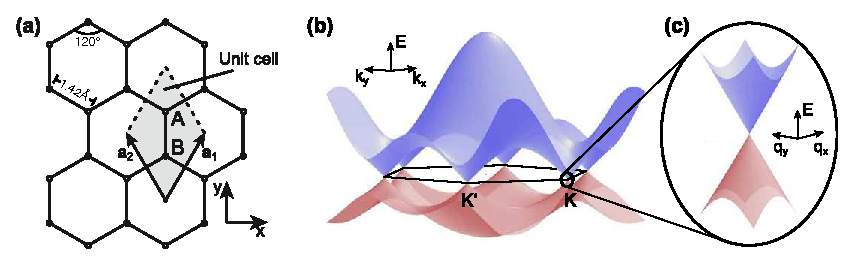
\includegraphics[width=\textwidth]{gra_lat_band.eps}
\caption[Graphene lattice and band structure.]{(a) Graphene honeycomb lattice composed of A and B hexagonal Bravais sublattices. (b) Band structure of graphene where CBM and VBM touch each other only at the $K$ and $K'$ points. (c) Approximately linear dispersion at $K$ and $K'$ point. Image source: \cite{Guttinger2012}. }  
\label{fig:gra_band}
\end{figure} 

Graphene delivers more than just an interesting electronic properties. For example, evidencing extraordinary mechanical properties graphene has a Young modulus $E = 1$Tpa and intrinsic strength of 130 Gpa\cite{Lee385}. This marks the strongest material ever measured. More than 300 times stronger than steel and four times harder than diamond. Carrier high mobility is another exciting feature that has more applicative importance in electronic devices. Free standing Graphene without subtract attached have been reported to have a highest mobility of 230,000 $cm^2/Vs$ at low temperature\cite{Bolotin2008a} and 120,000 $cm^2/Vs$ at 240 Kelvin, the latter value is higher than any known semiconductor\cite{Bolotin2008b}.
















 
\section{Post-graphene Materials}
\subsection{Functionized Graphene}
\subsubsection{Graphane}
\subsubsection{Fluorographene}
\subsection{Boron Nitride}
\subsection{Silicene and Germanene}
\subsection{Transition Metal Dichalcogenides}
\section{0D and 1D from 2D: buckyballs, nanotubes and nanoribbons}
\section{Synthesis methods}

%!TEX root = ../thesis.tex
%*******************************************************************************
%****************************** Second Chapter *********************************
%*******************************************************************************

\chapter{Computational methods}

\ifpdf
    \graphicspath{{Chapter2/Figs/Raster/}{Chapter2/Figs/PDF/}{Chapter2/Figs/}}
\else
    \graphicspath{{Chapter2/Figs/Vector/}{Chapter2/Figs/}}
\fi

\section{Theory}
\subsection{Density Functional Theory}
\subsection{Exchange-correlation functional}
\subsection{Jocob's ladder}
\section{Implementation}
\subsection{Basis set, Plane wave energy cut-off, K-points}
\subsection{Software Packages}
%!TEX root = ../thesis.tex
%*******************************************************************************
%****************************** Second Chapter *********************************
%*******************************************************************************

\chapter{General physical properties of 2D materials \label{chap:3}}

\ifpdf
    \graphicspath{{Chapter3/Figs/Raster/}{Chapter3/Figs/PDF/}{Chapter3/Figs/}{Chapter3/Figs/Vector/}}
\else
    \graphicspath{{Chapter3/Figs/Vector/}{Chapter3/Figs/}}
\fi

In this thesis, the properties of materials are divided into a preliminary and an advanced category, where the latter will be presented in the next chapter as the main results of this thesis. In this chapter, I will focus on the preliminary properties of 2D materials, namely structural, electronic, vibrational and mechanical properties. These properties can be used to test the methodology and form the foundation upon which the advanced properties are calculated. They are composed both of my original calculations and results from literature. An emphasis will be on the characteristic properties of 2D materials that are different from 3D cases.

\section{Structural properties}
\subsection{Layer structure}

As discussed in the \fullref{chap:1}, layered bulk materials are closely related to 2D materials. The strong anisotropic structure in the former results in the layer concept in the latter, and a single layer of a layered bulk material is a 2D material. This anisotropic nature is attributed to the weak interlayer bonds and the strong intralayer bonds. Van der Waals (vdW) interactions \cite{vdws} are the main source of these weak interlayer bonds. vdW interactions consist of the attraction and the repulsion between atomic or molecular entities caused by dipole-dipole, dipole-induced dipole and instantaneous induced dipole-induced dipole forces. The definition is sometimes extended to include all dispersion forces between molecules.  For 2D materials, vdW interactions become important as the number of layers is larger than one; that is few-layer materials having typically less than ten layers. They also belong to the family of 2D materials since the thickness of the materials is still small for quantum confinements to dominate their roles. As in its layered bulk counterpart, a few-layer system is a stack of monolayers hold together through vdW forces. When no other bonding types are present, interlayer vdW interactions determine all the change coming from going above a single layer, but this impact on the electronic structure can be significant. For example, from monolayer to bilayer, the linear dispersion relation of energy $E$ as a function of $k$ around the $\mathrm{K}$ k point evolves into parabolic-like spectrum\cite{Partoens2006,Mak2010a}. 

\begin{figure}[ht] 
\centering  
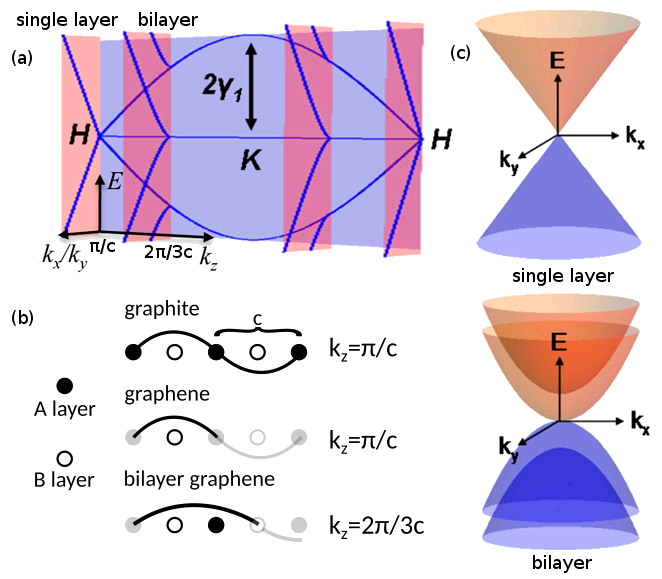
\includegraphics[width=0.9\textwidth]{gra_band.png}
\caption{(a) Energy-momentum dispersion relations of single layer and bilayer graphene as approximated by plane intersections of 3D graphite dispersion relation and (b) their 3D dispersion relations around the $\mathrm{K}$ k point. (c) Matching of the wavelength in graphite to that in single layer and bilayer graphene. Image adapted from: \cite{Mak2010a}. }  
\label{fig:gra_bands}
\end{figure} 

In \autoref{fig:gra_bands} (a), the dispersion relation of graphite along the z direction, that is the HKH line in the Brillouin zone, is shown on the blue plane. This direction is perpendicular to the graphite layers. Because of the quantum confinements in a few-layer system, the number of wave vectors that standing waves can take is limited.  If only the intralayer and interlayer interactions between the nearest neighbour atoms were considered, the dispersion relation in few-layer graphene can be approximated as those on the cross-section of virtual planes (the red planes in \autoref{fig:gra_bands} (a)) with the 3D graphite dispersion relation.  These planes are perpendicular to the z direction and intersect with the HKH line at limited points. This is called the quantization\footnotemark\footnotetext{sometime it is also referred as zone-folding} of dispersion relations\cite{saito1998physical}. These points are illustrated in \autoref{fig:gra_bands} (c). Under the condition that quantum confinements in a few-layer system require that the wave functions vanish at the imaginary layer right outside the surface of the system, the systems will have well-defined wave vectors. Then, the dispersion relations of graphene and bilayer graphene will be on the red planes that intersect the HKH line at $k_z=\pi/c$ and at $kz=2(\pi/3c)$, respectively.  Having the knowledge of the 3D band structure of graphite, one can approximate the dispersion relation of few-layer systems in this way. As shown in the red plane in \autoref{fig:gra_bands} (a) and the 3D version in \autoref{fig:gra_bands} (b), graphene has a linear dispersion relation and bilayer graphene has two parabolic-like bands that come from each layer. Moreover, the bilayer structure will never pass through the H point where graphene has passed to have a linear dispersion relation. This is because the standing waves in a bilayer will have a wave vector $k=2(n \pi/3c)$, where $n$ is a positive integer: 1, 2, ... , n. This will never be equal to $\pi/c$ for any integer number of $n$. More generally, systems with an even number of layers will not have a linear dispersion relation, and vice versa for systems that have an odd number of layers. Further, if other interactions were considered, an overlap of those bands touching each other would have occurred\cite{Partoens2006}. This overlap increases with the number of layers. Eventually, maximum overlap is reached in graphite.


\begin{figure}[htbp!] 
\centering  
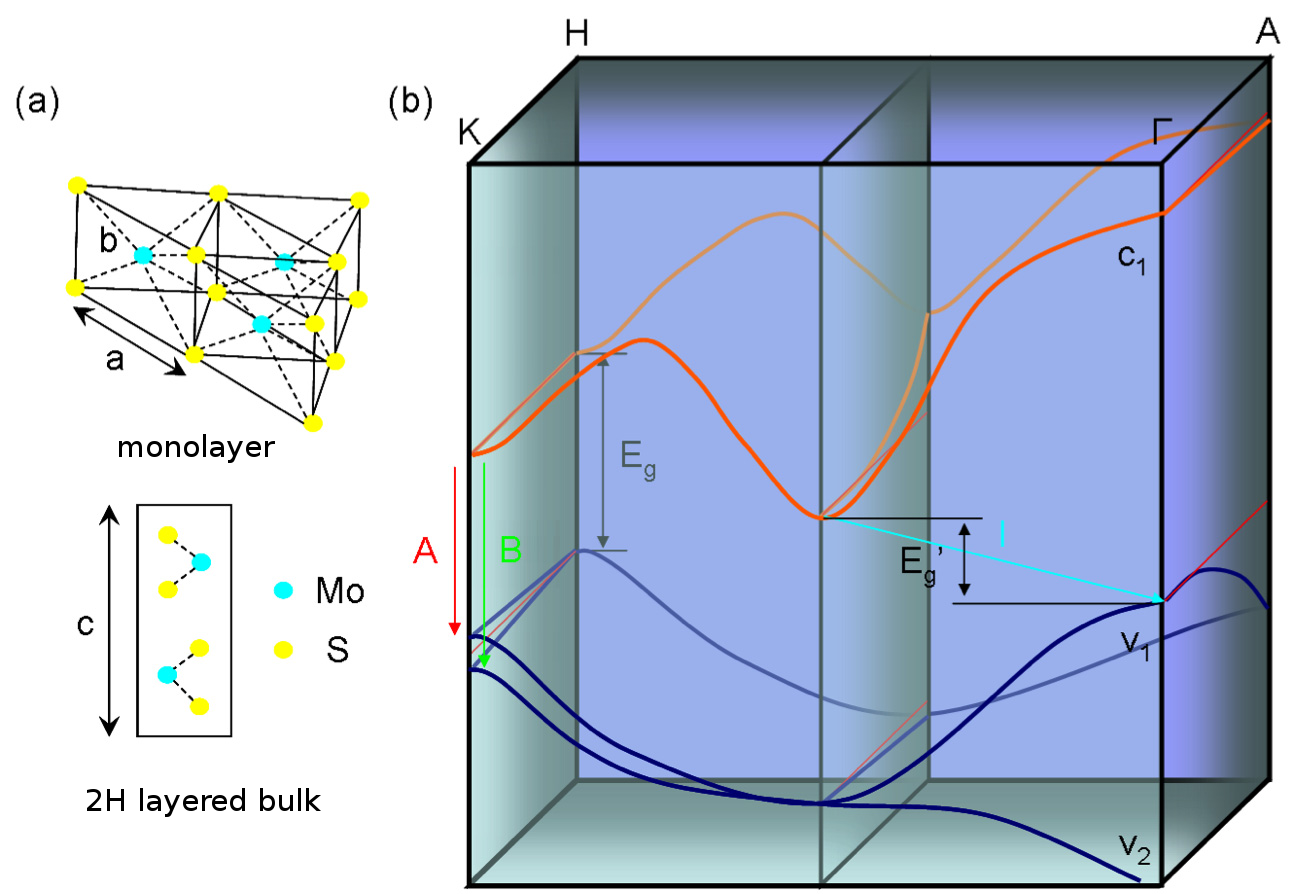
\includegraphics[width=0.8\textwidth]{mos2_band.png}
\caption{Energy-momentum dispersion relations of MoS$_2$ as plane intersections of 3D dispersion relations. Image adapted from: \cite{Mak2010}. }  
\label{fig:mos2_band}
\end{figure} 

Another example of the importance of interlayer interactions in few-layer 2D materials is seen for MoS$_2$. As mentioned in \fullref{chap:1}, as going from layered bulk to monolayer, MoS$_2$ transforms from an indirect band gap to a direct one. Here again, we can make use of the quantization scheme to approximate the band structure of the monolayer from that of the layered bulk. The monolayer and the layered bulk structure of 2H phase are shown in \autoref{fig:mos2_band} (a). In figure (b), let us focus on the planes parallel to the page that pass through the $\mathrm{K}\Gamma$ line and the HA line (simply call them $\mathrm{K}\Gamma$ plane and HA plane below). Similar to the previously discussed graphite, 2H layered bulk MoS$_2$ has two layers per unit cell. Therefore, according to the standing wave arguments that we have used for the graphene case above, HA plane represents the monolayer. $E_g$ and $E\prime_g$ are the band gaps of the monolayer and the layered bulk structures. Here, not only the magnitude of the band gap is increased as going from layered bulk to monolayer, the character of the band gap has changed as well. It is clearly shown that this is due to the band edges shifting. VBM at $\Gamma$ and CBM at the middle of $\Gamma\mathrm{K}$ line are brought closer as they go from monolayer to layered bulk. This corresponds to the widening of the band width and it is coming from the splitting of the VB and CB when more and more layers interact with each other through the interlayer interactions. Therefore, band gap in the layered bulk is defined by these two band edges, which in the monolayer was defined by band edges at $\mathrm{K}$. In contrast to this, the band edges at the $\mathrm{K}$ are not affected too much by the interlayer interaction to make a difference. So why do the band edges react differently to the interlayer interactions? If we look into the orbital composition of the band edges, we will find the ones that have widened the most, i.e. VBM at $\Gamma$, have the largest contribution from S $p_z$ and Mo $d_{z^2}$ orbitals. These out-of-plane orbitals are orientated vertically to the plane and thus have maximum overlap with the others from an adjacent layer. Therefore, band splitting is more profound for these band edges and causing the increase of their band width. In contrast, both the CBM and VBM at $\mathrm{K}$ are largely composed of S $p_x$ and $p_y$ orbitals and Mo $d_{xy}$ and $d_{x^2-y^2}$ orbitals. All of them are in-plane orientated orbitals and thus have limited effect from interlayer interactions\cite{Padilha2014}.

\subsection{sp hybridization\label{sphyb}}

After discussing layered structures and the importance of interlayer interaction, let us look into some details of the in-plane structures and how sp hybridization gives rise to various structures for 2D materials. When atoms come together to form bonds, the orientations of bonding orbitals are decisive for the final structure. The hybridization of s and p orbitals is a good example of this.  It mainly exists in three different variants: sp, sp$^2$ and sp$^3$, see \autoref{fig:sp_hybrid}. The hybridization index $n$ in sp$^n$ stands for the relative amount of p character in the resulting hybridized orbital. For example, sp$^2$ has 1/3 s character and 2/3 p character. Hybridized orbitals tend to maximize their distance to reduce the energy raised by the repulsion of electrons. As shown in \autoref{fig:sp_hybrid}, this results in tetrahedral structure of sp$^3$ orbitals, as in diamond, trigonal planar structure of sp$^2$ orbitals, as in graphene or graphite and linear structure of sp orbitals, as in ethyne molecules.  This is, for example, useful to explain the buckled structure of graphane and fluorographene. Because of sp$^3$ character developed when the fourth electrons are bonded with H or F atoms, buckling appears in these systems. 

\begin{figure}[htb] 
\centering  
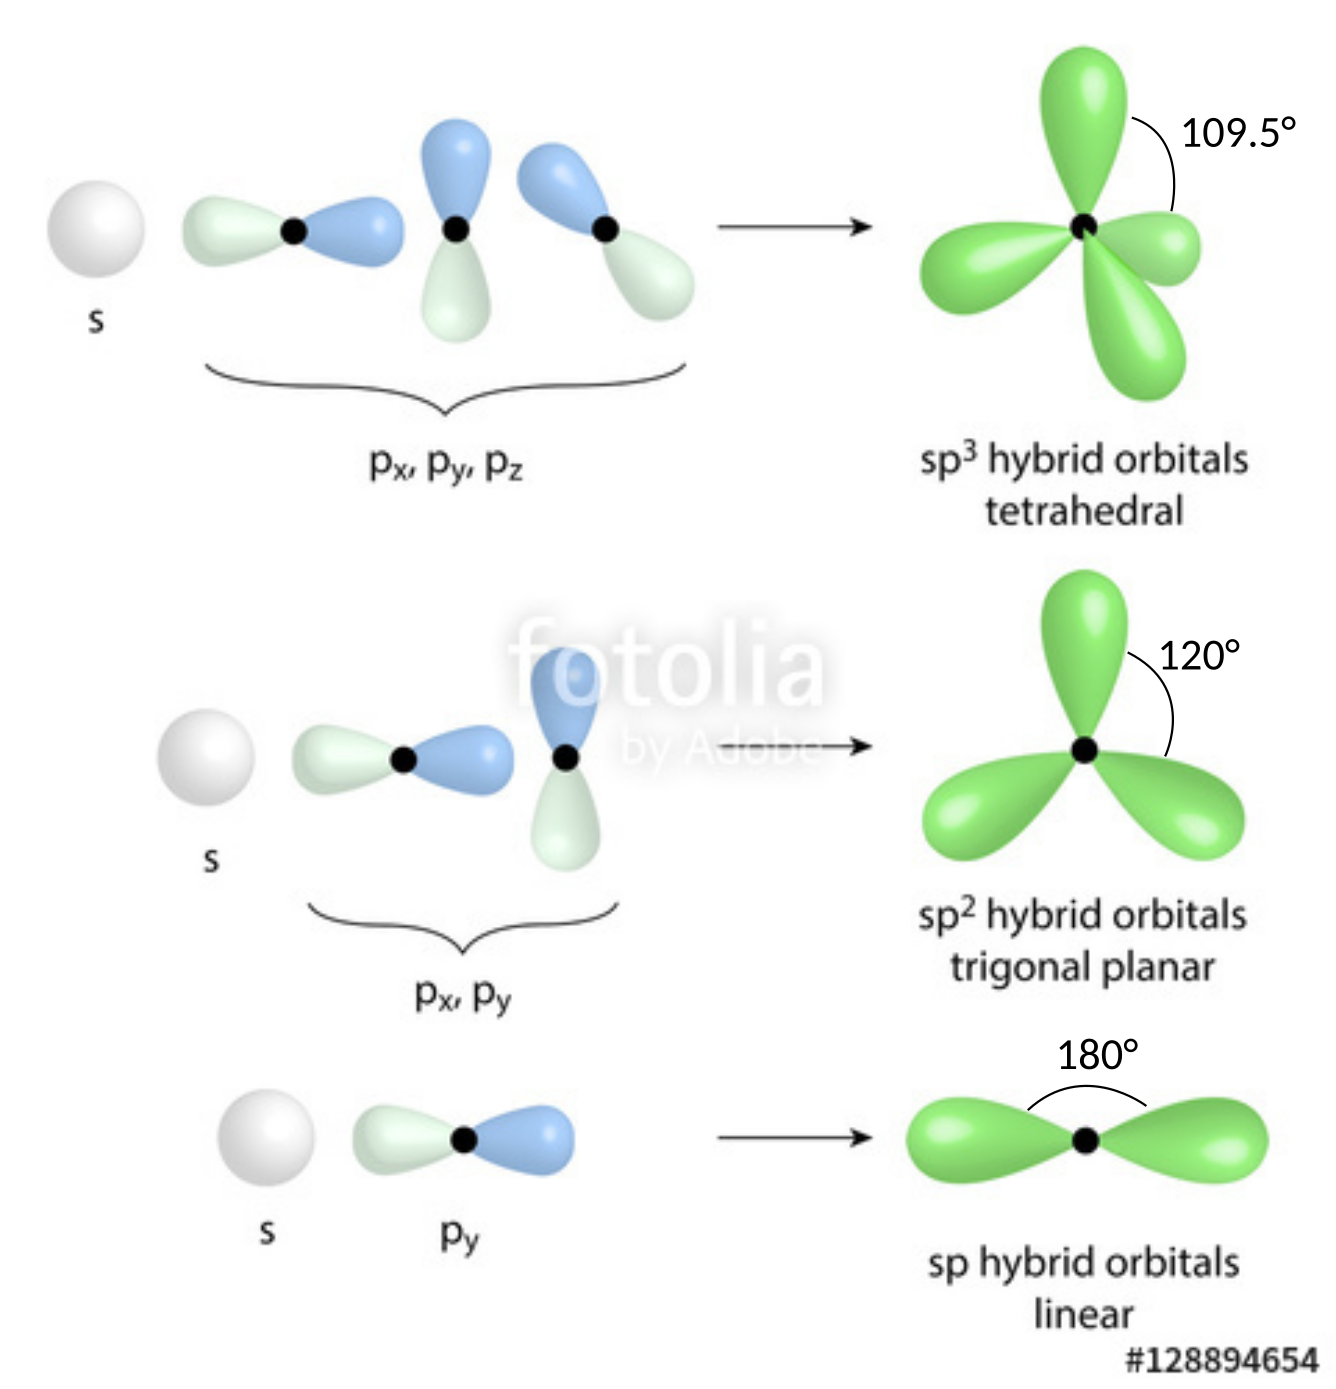
\includegraphics[width=0.8\textwidth]{sp_hybrid.png}
\caption{Three types of sp hybridized orbitals. Image adapted from: \cite{sp_hybrid}. }  
\label{fig:sp_hybrid}
\end{figure} 

\citet{coulson1949} generalized the relation of bond angle with $n$ as follows:
\begin{equation}\label{coulson}
1=-\sqrt{n_1n_2}~cos\theta_{12}, 
\end{equation}
where $\theta_{12}$ is the bond angle between orbital 1 and 2. The bond angle can be measured in the structures after the relaxation simulations. If orbital 1 and 2 have different $n_1$ and $n_2$, we still need one more constraint to solve the \autoref{coulson} for the hybridization indices $n$. This constraint is that, in the case of carbon atoms, the total portion of s orbitals should equal to 1, while it should be 3 for the p orbitals. With these pieces of knowledge, the \autoref{coulson} can be solved, and each orbital from one atom can be assigned with a $n$. This formula is useful to determine the s and p fractions of the bonds. For example, $\theta_{12}=90^o$ gives $n\rightarrow\infty$, which means it is a pure p orbital; $\theta_{12}=120^o$ gives $n=2$, that is a sp$^2$ hybridized orbital. Generally, the wider the bond angle,the larger the s contribution. Accordingly, bond angles are ordered as sp > sp$^2$ > sp$^3$. Of course, the \autoref{coulson} is more useful when the bond angle takes values other than those three types of hybridized orbitals mentioned, then it can be used to explain the resulting geometry.

\section{Electronic properties}

The electronic properties are among the first features we would like to know of new materials, not only because semiconductor and metal have different roles in the applications, but also because details of the electronic structure set the direction for further exploration. One example from my experience is that by monitoring electronic structure variations under strain, we can predict how the mobility of the carriers can be tuned. This will be discussed in later chapters. Therefore, it is important to understand this property of a new material to fully reveal its potential. Electronic properties are usually characterized by the band structure (BS) and density of states (DOS). These calculations are standard calculations in common first-principles codes from where all subsequent calculations start. After solving the Kohn-Sham equation with properly defined cut-off energy, k points etc., we will have the eigenenergy of each state, indexed by a k point in the Brillouin zone and a band number.  The DOS is a count of such states at a specific energy. The BS is the plot of the eigenenergies along lines in the Brillouin zone that connect high symmetry k points.  2D materials have a vast variation of electronic properties, from semimetallic graphene to semiconducting MoS$_2$ and insulating BN. I will briefly discuss this at the end of this section. The purpose of this section is to point out some of the interesting electronic properties of some 2D materials. We will start with a brief introduction of the electronic properties of graphene.

\subsection{Graphene}

As mentioned before, the orbitals of the C atoms in graphene are sp$^2$ hybridized. Each one of these sp$^2$ orbitals, coloured in green in \autoref{fig:gra_bond}, is composed of s, p$_x$ and p$_y$ orbitals, whereas the p$_z$ orbital, coloured in yellow in the figure, is left unchanged. One sp$^2$ hybridized orbital with another one from an adjacent atom form a strong $\sigma$ bond, while $p_z$ orbitals form $\pi$ bonds. It may look like alternative single and double bonds between atoms, however, according to Clar's theory, the bond order, i.e. the number of chemical bonds between a pair of atoms, in graphene is 4/3 and is uniform\cite{Wassmann2010}. This has to do with the high symmetry of the graphene lattice.

\begin{figure}[htbp!] 
\centering  
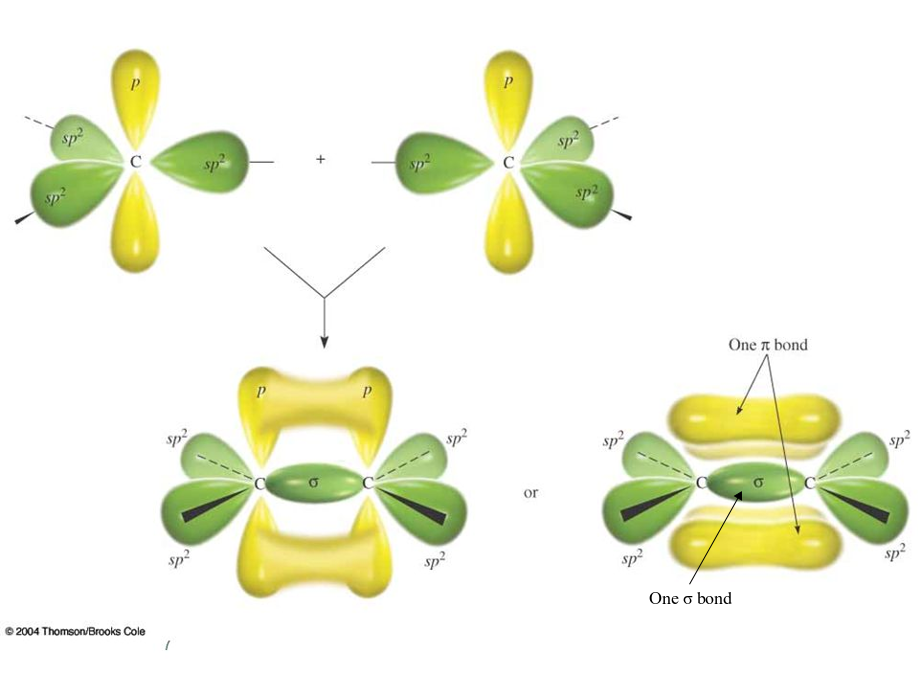
\includegraphics[width=0.7\textwidth]{double_bond}
\caption{The formation of $sp^2$ $\sigma$ and $p_z$ $\pi$ double bond. Image source: \cite{gra_bond}. }  
\label{fig:gra_bond}
\end{figure} 

Every C atom has the same local environment in graphene. However, adjacent atoms are not equivalent from the symmetry point of view. They belong to different hexagonal sublattices, $A$ and $B$, as indicated with blue and yellow colors in \autoref{fig:gra_lat}. $a_1$ and $a_2$ are the basis vectors in real space connecting equivalent lattice sites. On the left, $b_1$ and $b_2$ are the basis vectors in reciprocal space connecting equivalent k points. The hexagon in the reciprocal space is the first Brillouin zone where all inequivalent k points are contained. These k points correspond to different parallel lines of atoms and thus their directions in the reciprocal space are associated with different directions in real space. The k wave vectors near the $\Gamma$ point have longer wave length than those away from it. While those at the boundary of the first Brillouin zone have wave lengths that are two times the unit cell dimension on the direction specified by the k points. For example, the most interesting k points for graphene are the $\mathrm{K}$ and $\mathrm{K}'$ points. These directions correspond to the $a_1$ and $a_2$ directions in real space. It is only at these k points in the Brioulloin zone that the antibonding and the bonding $\pi$ bands touch each other.  

\begin{figure}[htbp!] 
\centering  
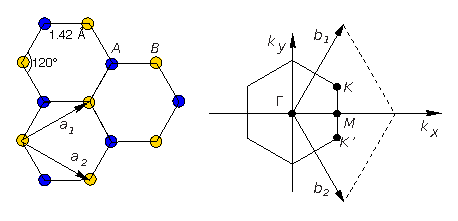
\includegraphics[width=0.8\textwidth]{gra_lat.eps}
\caption{Graphene lattice and its Brillion zone. Image source: \cite{CastroNeto2009}. }  
\label{fig:gra_lat}
\end{figure} 

As compared to $\pi$ bonds, the $\sigma$ bonds originate from a strong overlap of $sp^2$ orbitals. The interaction is so strong that the splitting of bonding and antibonding orbitals is large. This makes the $\sigma$ bonding orbitals deep in energy, or in other words, makes the $\sigma$ bond strong and difficult to break. This feature contributes the most to the mechanical strength of graphene. On the other hand, $p_z$ orbitals are less overlapping. This makes the $\pi$ bond energy close to Fermi level, i.e. the highest occupied state. Therefore, they contribute the most to the electronic properties of graphene.  


\subsection{Dirac cone and symmetry}

We have seen that graphene, silicene and germanene have an interesting electronic structure: forming a Dirac cone. We also have listed the consequences of having such a feature: high mobility, massless carriers etc. In this section, we will discuss the symmetry condition for the existence of Dirac cones. This knowledge can be used to discover more materials with Dirac cone. 
\begin{figure}[htbp!] 
\centering  
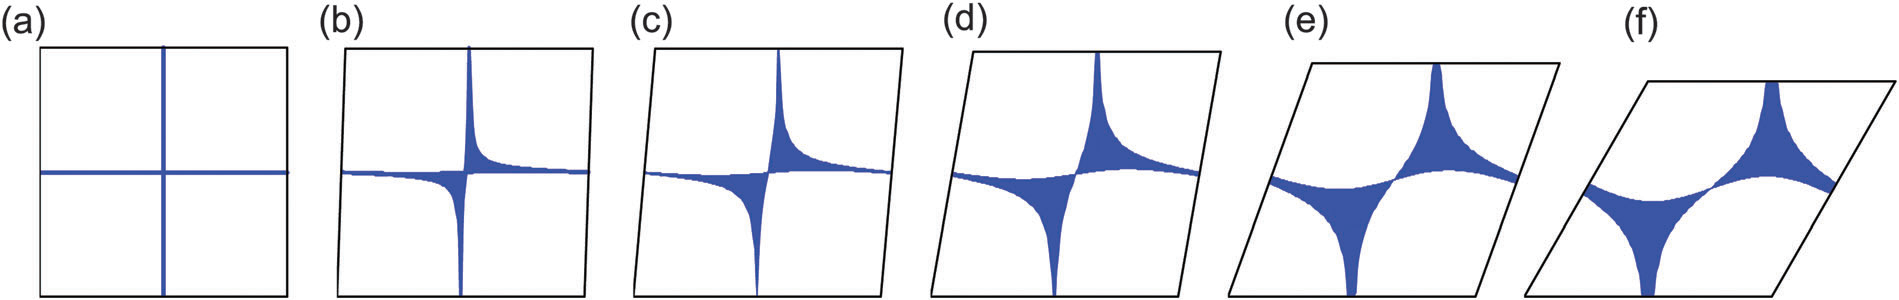
\includegraphics[width=0.95\textwidth]{dirac_hs.png}
\caption{Possible positions for the second atom (blue area) in order to guarantee the existence of Dirac cones as going from (a) square lattice to (f) hexagonal lattice. The first atom is located at the corners of the unit cell. Image source: \cite{Liu2013}. }  
\label{fig:dirac_hs}
\end{figure} 
According to the von Neumann-Wigner theorem, the space-time inversion symmetry is crucial for the existence and protection of Dirac cones\cite{Wang2015b}. It is a combination of space inversion and time reversal symmetries. These two are equally important and have to act simultaneously for the possible formation of Dirac cones. A more restrictive condition that guarantees the existence of Dirac cones has to deal with relations of hopping integrals\cite{Hasegawa2006,Liu2013}. A study by \citet{Liu2013} revealed that the hexagonal lattice has the most favourable structure to form Dirac cones. The probability decreases as one goes from a hexagonal lattice to a square lattice, as shown in \autoref{fig:dirac_hs}. Therefore, since most of the 2D materials have hexagonal symmetry, there will be a higher chance of finding materials with Dirac cones in this category.

\subsection{Examples: 2D-h-BN, 2D-MoS$_2$ and graphene}
\begin{figure}[htbp!] 
\centering  
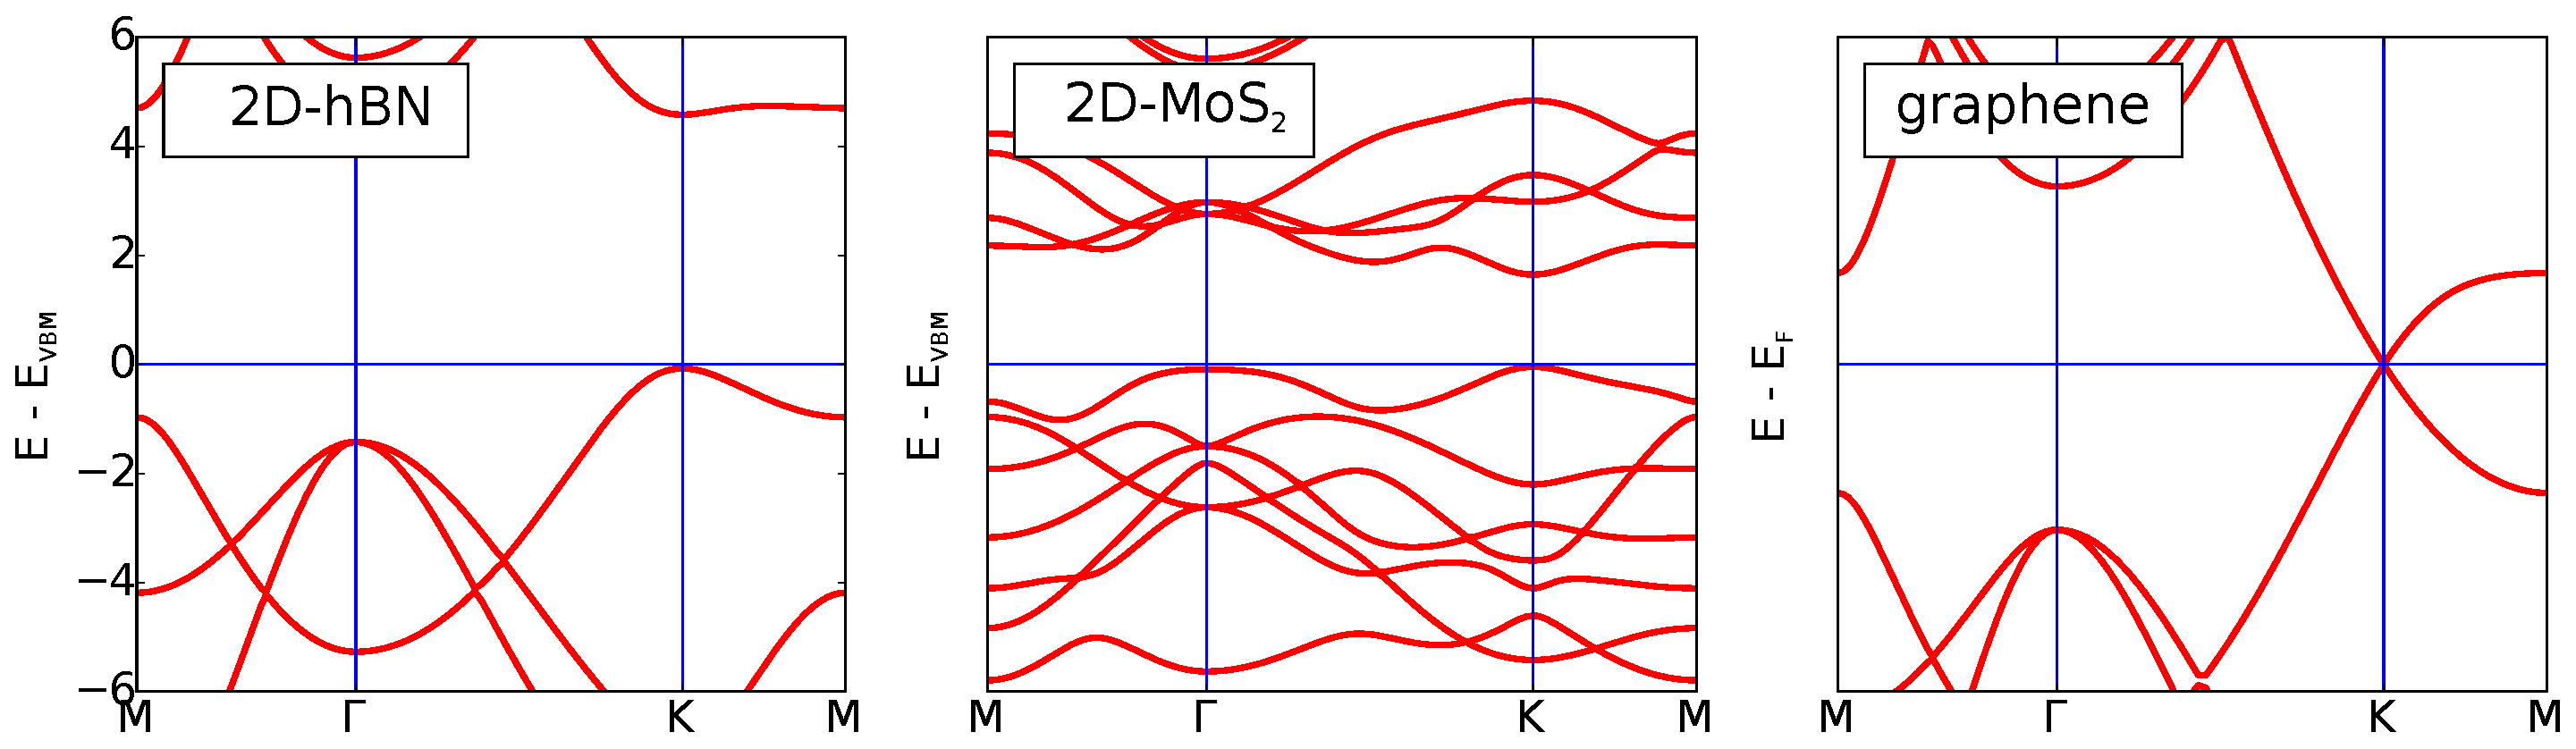
\includegraphics[width=\textwidth]{bss.eps}
\caption{Electronic band structures of 2D-hBN, 2D-MoS$_2$ and graphene calculated with PBE-GGA functional. }  
\label{fig:bss}
\end{figure} 
Three typical examples of the band structures of 2D materials are shown in \autoref{fig:bss}. The 2D h-BN acts as an insulator due to a large band gap in the ultraviolet range, therefore it is suitable to serve as a dielectric layer in an electronic device. The 2D TMDs have a band gap ranging from 1.0-2.5 eV which is in the visible and the near infrared range of light, therefore, they are suitable for optoelectronic device applications. Furthermore, as we compare the dispersion curves along the $\mathrm{M}\Gamma$ and $\mathrm{K}\Gamma$, we can see that the electronic structures are generally the same on these paths which correspond to different crystallographic directions. This means the materials in the figure are highly isotropic, thus we would expect the same for the physical properties. In the results chapters of this thesis, we will see some new 2D materials that are highly anisotropic. Their discoveries enrich the features of the physical properties of 2D materials.

\section{Vibrational properties}

The vibrational properties form an important aspect of materials, especially at finite temperature. Thermal expansion, thermal conductivity and electron mobility are all vibrational related topics. Therefore, it is crucial to understand the characterization of this in computational modelling. The force on an atom can be calculated from the wave functions evaluated from DFT thanks to the Hellmann-Feynman theorem. When searching for the equilibrium geometry of the materials, one basically tries different positions of atoms to find a geometry that minimizes all the forces. This usually is the first thing to do for new materials, since different codes, implementations and, more importantly, different functionals will give different results. Despite the fact that the difference is usually small, an unrelaxed geometry will have residual forces on the atoms. This is particularly important when vibrational properties are concerned. Vibrational properties are characterized through the energy (usually expressed in terms of frequency) versus vibrational wave vector dispersion relations.  In crystals,  all atoms vibrate around their equilibrium positions. The vibrational modes are quantized into phonons. Each phonon represents a periodic, collective vibration with a well-defined vibrational mode and wave vector. The forces ($F$) that restore the atoms when they deviate from their equilibrium positions can be calculated from DFT either by introducing small displacement or from perturbation theory. Then, the force constants, $\Phi$, can be constructed by monitoring the change in forces through the displacements, $u$, of atoms in the following way:

\begin{equation}
\Phi_{i\alpha,j\beta}= \frac{\partial F_{j\beta}}{\partial u_{i\alpha}},
\end{equation} 
where the $i,j$ indices are the labels for atoms, $\alpha,\beta$ are the Cartesian directions: $x$, $y$ and $z$. The Fourier transformation of the force constants at wave vector $\mathbf{q}$ is the dynamical matrix $D(\mathbf{q})$ that is related to the frequency of the phonon through the eigenvalue problem:

\begin{equation}\label{eqa:w_q}
\omega^2(\mathbf{q},n)\mathbf{e}(\mathbf{q},n)=D(\mathbf{q})\mathbf{e}(\mathbf{q},n),
\end{equation}
where $\omega(\mathbf{q},n)$ is the frequency of the phonon in mode $n$ having a wave vector $\mathbf{q}$, and $\mathbf{e}(\mathbf{q},n)$ is the eigenvector\cite{Ackland1997,Parlinski2011}.  Depending on whether atoms in the unit cell are vibrating in-phase or out-of-phase, phonon modes are categorized into acoustic and optical, respectively. For polar materials, charged atoms that vibrate with respect to each other can interact with light, which is the reason that these types of vibrations are called optical modes. Further, considering the respective directions of the wave ($\mathbf{e}$) and vibration ($\mathbf{q}$), the modes are subcategorized into transverse optical (TO) modes and transvers acoustice (TA) modes, where $\mathbf{q} \perp \mathbf{e}$), and longitudinal optical (LO) and longitudinal acoustic (LA) modes, where $\mathbf{q} \parallel \mathbf{e}$. These modes are all in-plane vibrations for 2D materials. For 2D materials, another direction is different from those in-plane ones, namely the $\mathbf{c}$ lattice vector direction perpendicular to the 2D plane. Special modes exist: out-of-plane transverse optical (ZO) and out-of-plane transverse acoustic (ZA) ($\mathbf{q} \perp \mathbf{e}$ and $\mathbf{q} \parallel c$). The total number of acoustic modes is three, that of optical modes is 3N-3, where N is the total number of atoms in the unit cell. 


\subsection{Example: 2D-MoS$_2$}

Let us now take layered bulk and monolayer MoS$_2$ as examples to highlight some of the important details of phonon dispersion relations. A comparison of vibrational modes between layered bulk and monolayer MoS$_2$ is presented in \autoref{fig:mos2_ph} (a). First of all, the number of atoms in the unit cell reduces from six to three from layered bulk to monolayer. Therefore, the number of the optical modes will be reduced as well from 15 in the layered bulk to six in the monolayer. In the \autoref{fig:mos2_ph} (a) it is shown, as the material is transformed to the monolayer, several modes merge with others that only differ by whether the vibration in different layers is in-phase or out-of-phase. Secondly, a characteristic feature of phonon disperions for layered bulk and 2D materials has appeared, namely the quadratic ZA mode (flexural mode). It is usually linear in 3D bulk materials because of strong interlayer interactions. Because in layered bulk, the interlayer interactions are weak and absent in 2D materials, therefore, it will cost less energy for the out-of-plane vibration and the quadratic dispersion will appear\cite{kittel}. This feature is closely related to the formation of the intrinsic ripples in 2D materials, e.g. graphene\cite{neek} and MoS$_2$\cite{mos2-ripple}. As shown in \autoref{fig:mos2_ph} (b), phonons with longer wave lengths, i.e. around $\Gamma$, in ZA mode have smaller frequencies or energies. This means this mode is more easily excited at low temperature and forms ripples which can be often observed in 2D materials. The formation of ripples is crucial for the stability of 2D materials at a finite temperature. Lastly, in the projected DOS, the projections of mode eigenvetors to in-plane (XY) and out-of-plane (Z) components are shown. The modes with Z components, i.e. ZO$_1$, ZO$_2$ and ZA, contribute the most to the Z projections, and vice versa for the longitudinal and acoustic modes to XY projection. 

\begin{figure}[htbp!] 
\centering  
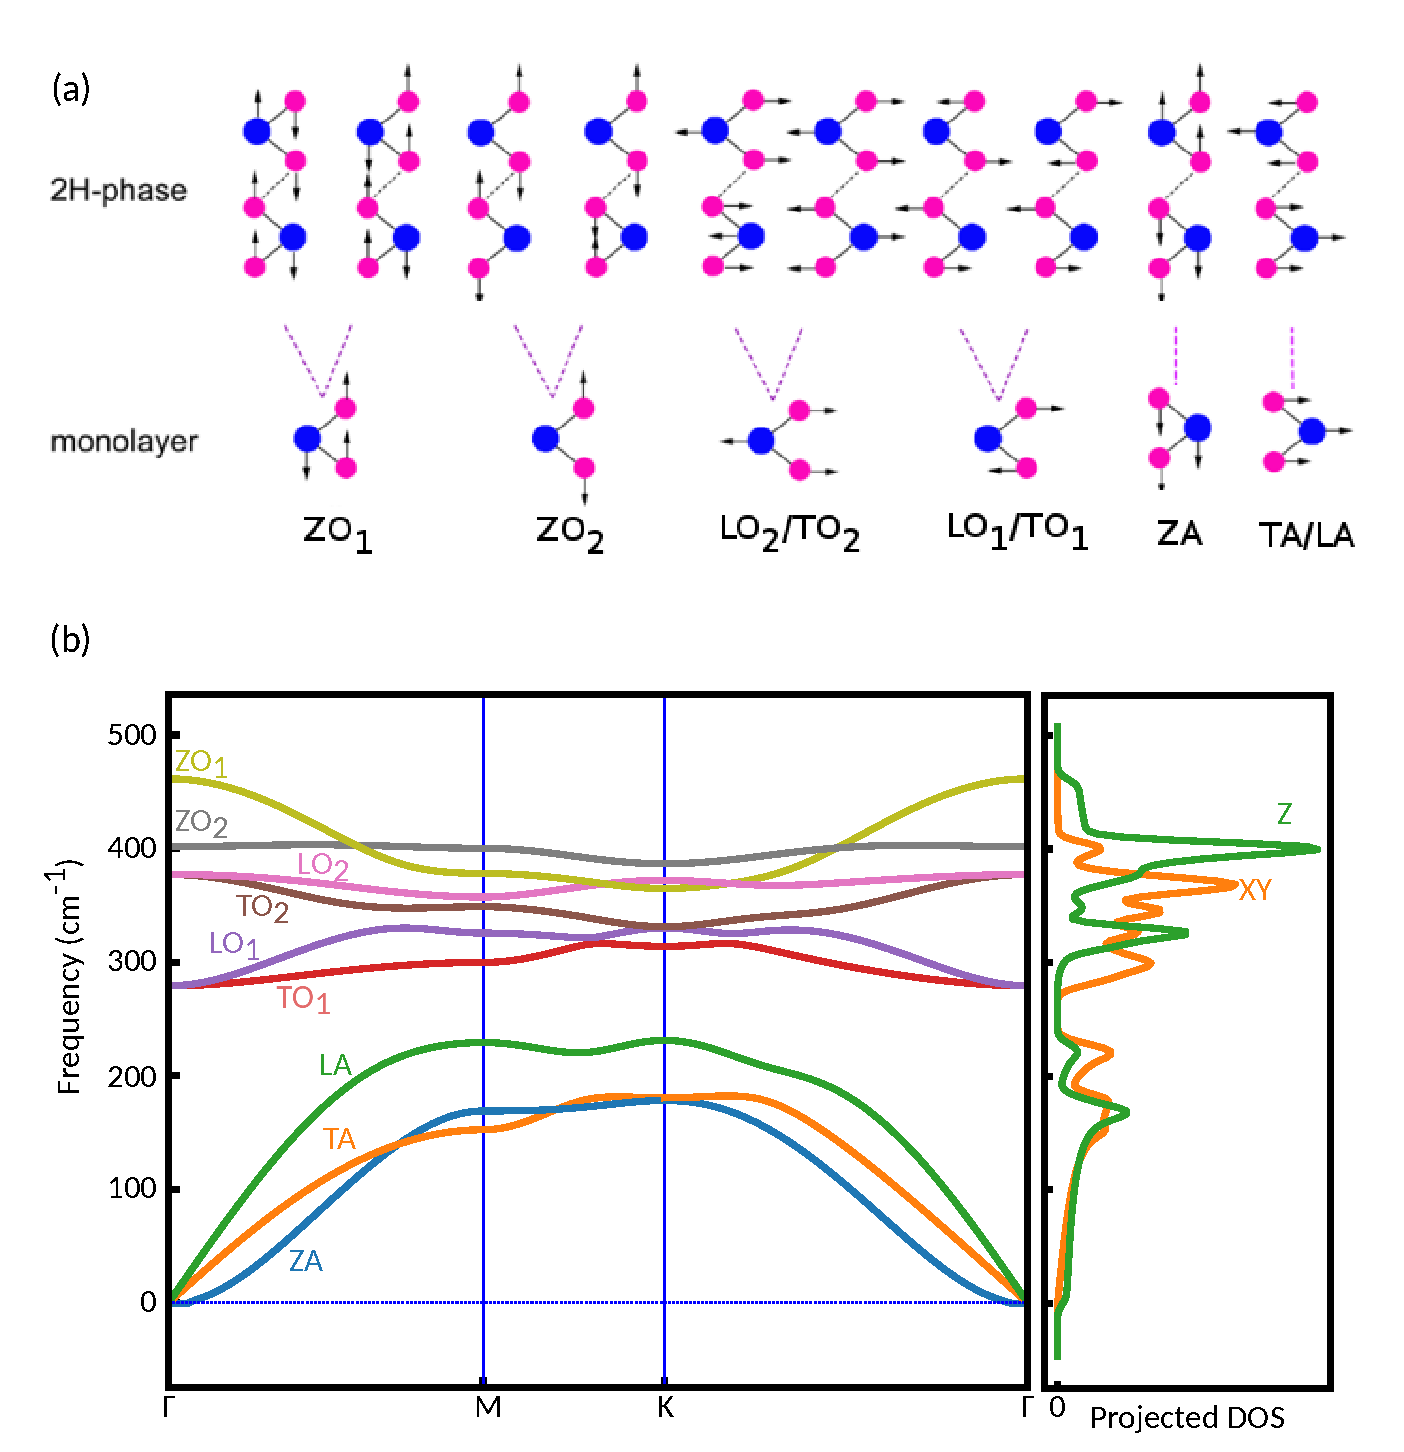
\includegraphics[width=0.8\textwidth]{ph_mos2.eps}
\caption{(a) phonon modes of layered bulk (first row) and monolayer (second row) MoS$_2$ at $\Gamma$ q point. (b) phonon dispersion and projected DOS of monolayer MoS$_2$.}  
\label{fig:mos2_ph}
\end{figure} 


\subsection{Dynamic stability from phonon dispersion}

One of the most useful features of the phonon dispersion is the possibility to check the dynamical stability of the structure. An unstable structure is usually indicated by the presence of imaginary frequencies in the phonon spectrum in some part of the Brillouin zone, see \autoref{fig:img_band} for example. 


\begin{figure}[htb] 
\centering  

\includegraphics[width=0.5\textwidth]{img_band.png}
\caption{ Imaginary frequencies are shown as negative frequencies in a phonon dispersion plot.}  
\label{fig:img_band}
\end{figure} 

\begin{figure}[htb] 
\centering  
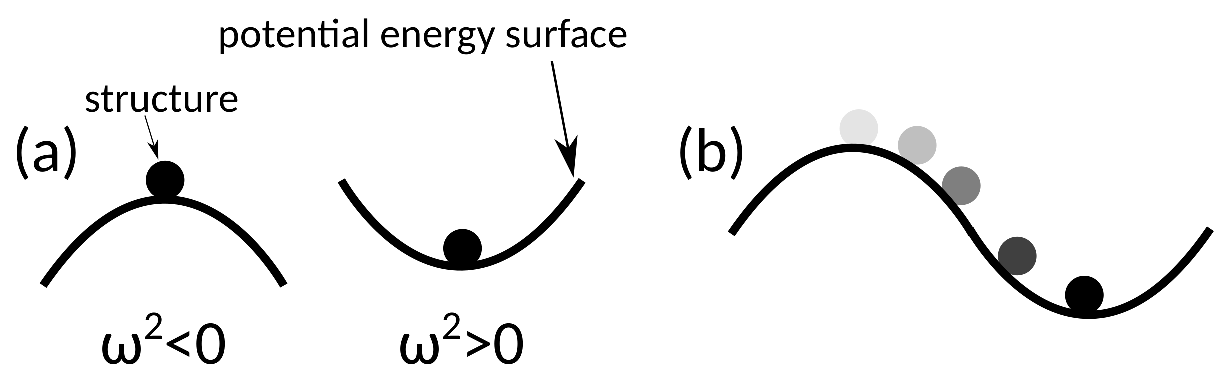
\includegraphics[width=0.7\textwidth]{fre_ima.eps}
\caption{ (a) A structure at the convex (left) and the concave (right) of the PES. (b) Searching for a stable structure (phase transition).}  
\label{fig:fre_ima}
\end{figure} 

Now let us try to understand this and make use of it to convert an unstable to a stable structure. Consider a relaxed structure in which the forces on all atoms have vanished. This could be locally at the maximum or the minimum of the potential energy surface (PES), see \autoref{fig:fre_ima}. Note that, in both situations, the forces, the derivative of the PES curves, are zero. Therefore, both situations can occur when the structure is relaxed only following the forces. In the case of a convex PES, the dynamical matrix $D(\mathbf{q})$ will have negative components because the direction of the force is the same as the displacement. We have seen from \autoref{eqa:w_q} that $D(\mathbf{q})$ is related to the square of the frequency $\omega$, hence imaginary frequencies are the only solutions. However, a structure with imaginary frequencies near $\Gamma$ q point does not necessarily mean it is not stable. Since a large supercell consisting of multiples of the unit cell is typically used to do phonon calculations, it may be that the size of the supercell is not large enough to correctly describe long wavelength phonons. In contrast to this, a structure with imaginary frequencies that appear around other q points than $\Gamma$ would imply a structure instability or a structural phase transition. The lowering of the energy with some vibrational modes means the structure prefers the modulation induced by the vibration, therefore if we calculate the energy of the modulated structure we will have a lower energy structure. With advanced techniques in phonon software\cite[e.g.][]{phonopya}, it is possible to perturb such a structure based on the vibration mode which has an imaginary frequency to find a lower energy state and stabilize the structure, as schematically illustrated in \autoref{fig:fre_ima} (b). 



\section{Mechanical properties}

In \fullref{chap:1}, we have seen the stiffness and strength of some of the 2D materials. These all belong to the mechanical properties of the materials. The force on the atoms or the stress $\boldsymbol{\sigma}$ on the the unit cells under a finite strain $\boldsymbol{\epsilon}$ are typical outputs from common first-principles codes. Within the elastic regime of the stress-strain relation, they can be related through the elastic constant $\boldsymbol{C}$: $\boldsymbol{\sigma}=\boldsymbol{C}\boldsymbol{\epsilon}$, this is Hook's law. $\boldsymbol{C}$ is a 6$\times$6 matrix whose matrix elements have a form $C_{ij}$. The elements measure the resistance of materials in the $i$ direction to a deformation in the $j$ direction, where $i$ and $j$ are the index of stress and strain tensors, respectively.  Under the Voigt notations, the indices have the following correspondence: 1$\rightarrow$ xx, 2$\rightarrow$ yy, 3$\rightarrow$ zz, 4$\rightarrow$ yz, 5$\rightarrow$ zx, 6$\rightarrow$ xy. The elastic constants can be simplified if the crystal symmetry and dimension are taken into account. For example, for 2D hexagonal lattice symmetry, Hook's law reads:

\begin{equation}
\begin{pmatrix} \begin{array}{c} \sigma_1 \\ \sigma_2 \\ \sigma_6 \end{array} 
\end{pmatrix}
=
 \begin{pmatrix}
  C_{11} & C_{12} & 0  \\
  C_{12} & C_{11} & 0  \\
  0 & 0 & (C_{11}-C_{12})/2
 \end{pmatrix}
 \begin{pmatrix} \begin{array}{c} \epsilon_1 \\ \epsilon_2 \\ \epsilon_6 
\end{array} \end{pmatrix}.
\end{equation} 

In this way, all elastic constants can be extracted from stress-strain data from first-principles calculations. Generally, it is more convenient to have one quantity to describe each aspect of the mechanical properties of materials. This is where the Young's modulus $Y$, shear modulus $G$ and Poisson's ratio $\nu$ become useful. Following the previous notations, they are defined as 

\begin{equation}
\begin{array}{c}

Y_\alpha=\frac{1}{S_{\alpha\alpha}},\hspace{6 pt} \alpha = 1, 2, 3
\end{array}.
\end{equation}

\begin{equation}
\begin{array}{c}
\nu_{\alpha\beta}=-Y_\beta S_{\alpha\beta},\hspace{6 pt} \alpha, \beta = 1, 2, 3 
\hspace{6 pt}(\alpha\neq\beta)
\end{array}.
\end{equation}

\begin{equation}
\begin{array}{c}
G_{\gamma\gamma}=\frac{1}{S_{\gamma\gamma}} ,\hspace{6 pt} \gamma = 4, 5, 6
\end{array},
\end{equation}
where $\boldsymbol{S}=\boldsymbol{C}^{-1}$ is the compliance matrix \citep[e.g.][]{nye1985physical}. The Young's modulus and shear modulus give the stiffness of the material when it responds to stretching and shearing deformation in particular directions and they stand for the hardness of the materials. Their unit in 2D is $J/m^2$ or $N/m$. To make them comparable with conventional 3D materials, 2D moduli usually are converted into 3D ones by dividing the former by the thickness of the sheet. Poisson's ratio gives the ratio of the transverse to the axial strain. It represents how easy it is to change the shape of the material with respect to changing the volume. Liquid and rubber have a Poisson's ratio close to 0.5, which is the theoretical upper limit of this quantity and making them the easiest materials to change shape over volume. In contrast, a cork has a Poisson's ratio close to zero, meaning zero lateral expansion when compressed in other directions. The breaking strength/strain is a measure of maximum load limit that materials can withstand and it is used to characterize how strong a material is. This quantity is usually obtained by continuously deforming the materials until they break and recording the maximum stress/strain. This can be done both experimentally and through simulations. 

\subsection{Examples: graphene, 2D-BN and 2D-MoS$_2$}

In \autoref{table:mech}, the mechanical properties of several 2D materials are shown, as well as that of steel for comparison.  As mentioned, graphene is the strongest material ever measured. This is due to its strong $\sigma$ and $\pi$ bonding. With similar bonding in BN, it shows comparable results to graphene. MoS$_2$ has lower stiffness and strength than the previous two due to weaker bonding, nevertheless, it is still much stronger than steel. The Poisson's ratio has an inverse relation with Young's modulus. This means graphene acts more like cork than rubber as compared to MoS$_2$. 

\begin{table}[htb]
\caption{Mechanical properties of graphene, BN and MoS$_2$}
\centering
\label{table:mech}
\begin{tabular}{l l l l }
\hline\hline
material &   Young's modulus  & Breaking strength  &  Poisson's ratio \\
         &   TPa              & GPa               & \\
\hline
graphene\cite{Lee385} &   1.0$\pm$0.1         & 130$\pm$10               & 0.149\cite{Kudin2001} \\
2D-BN \cite{Topsakal2010}      &   0.71\textendash 0.97        & 120\textendash 165           & 0.210\\
2D-MoS$_2$\cite{Bertolazzi2011}  &   0.27$\pm$ 0.10   & 23                & 0.29 \cite{Cooper2013}\\
A36 steel\cite{steel} & 0.2 & 0.4\textendash 0.55  & 0.26 \\
\hline\hline
\end{tabular}
\end{table}

\subsection{Mechanical stability: Born stability criteria}

Mechanical stability is a criterion for unstressed crystal stability, which is additional to dynamical stability. It was first pointed out by \citet{born_1940} in the 1940’s., for that, it is often called “Born stability criteria”. Its core concept is that the elastic energy should be positive for any non-zero strains. The elastic energy $U$ is related to the elastic constants $C_{ij}$ in the following way:

\begin{equation}
U=U_0+\frac{1}{2}V_0\sum_{i=1,j=1}^6 C_{ij}\epsilon_i\epsilon_j,
\end{equation}
where $U_0$ is the equilibrium energy and $V_0$ is equilibrium volume. According to Born's paper\cite{born_1940}, the necessary and sufficient stability conditions are: 1) $|\mathbf{C}|>0$; 2) all eigenvalues of $\mathbf{C}$ are positive; 3) Sylvester’s criterion: the determinants of the upper-left $k$ by $k$ sub-matrices are positive; (4) an arbitrary set of minors of $\mathbf{C}$ are positive. \citet{Mouhat2014} formulated closed form expressions of this criteria for different crystal systems. Taking into account the symmetry of these systems, the number of criteria reduces, and becomes very useful to check the mechanical stability of a new crystal system. For example, for a 2D hexagonal crystal, the criteria become:

\begin{equation}
C_{11}>|C_{22}|,C_{66}>0.
\end{equation}
%!TEX root = ../thesis.tex
%*******************************************************************************
%****************************** Second Chapter *********************************
%*******************************************************************************

\chapter{Results of Physical Properties Calculations in Novel 2D Materials \label{chap:4}}

\ifpdf
    \graphicspath{{Chapter4/Figs/Raster/}{Chapter4/Figs/PDF/}{Chapter4/Figs/Vector/}}
\else
    \graphicspath{{Chapter4/Figs/Vector/}{Chapter4/Figs/}}
\fi


\nocite{Yimamu2012,Aierken2015.porlandite,Aierken2015.thermalP,Aierken2015.nanotubes,Menderes2015,Aierken2016.mobility,Aierken2016.pentasilicene,Aierken2016.magnetism,Aierken2017.transport,Aierken2017.battery}


In this and the next chapter, the main results of the thesis will be presented. In \autoref{chap:1}, I have reviewed some of the early post-graphene 2D materials, and their physical properties in \autoref{chap:3}. As it has been defined, the properties discussed before belong to the basic property category. In this chapter, I will present my work on the determination of some of the advanced physical properties, namely thermal, piezoelectric, and magnetic properties and Li battery related properties. In addition, I will also introduce several new 2D materials: phosphorene, monolayer titanium trisulfide, penta-hexa-graphene and MXenes. Each of the sections below resulted in a research paper. 

\section[Thermal properties of black and blue phosphorene]{Thermal properties of black and blue phosphorene \footcite[This work is published:][]{Aierken2015.thermalP} \label{thermal_phos}}


\subsection{Introduction}

Black phosphorene (black P) is a single atomic layer of black phosphorus and has been successfully exfoliated \cite{Han2014,Li2014}. Similar to the multiphase structures in phosphorus, at least six different possible stable 2D allotropes of phosphorene were proposed\cite{Zhu2014,Guan2014a,Wu2015}. This multi-phase nature is because in contrast to the C atoms of graphene, the P atoms in phosphorene have $sp^3$-hybridized orbitals. This is mainly caused by the extra valence electron of P atoms in comparison to C atoms. Indeed, if this extra electron is placed in a $sp^2$-hybridized structure, they would occupy the energetically unfavourable (antibonding) $\pi^*$ band. However, with $sp^3$-hybridization, a $\sigma$-bond network can be formed with three $sp^3$ orbitals and the other $sp^3$ orbital is used to host the remaining electron pair. This leads to an essentially tetragonal coordination of the P atoms and results in a buckled nature of $sp^3$-hybridized sheets, see \autoref{fig:phos_struc} for the structures. The out-of-plane positions of the atoms in $sp^3$-hybridized sheets give rise to various possible structural phases which are absent in $sp^2$-hybridized systems. Among those, black P, also referred as the $\alpha$ phase, is the most stable allotrope. However, the cohesive energy of blue phosphorene (blue P), or the $\beta$ phase, is only a few meV/atom higher than that of black P, while other crystal structures are much less favourable with energy at least by $\sim$ 80 meV/atom higher.  

\begin{figure}[htbp] 
\centering
\includegraphics[width=0.8\linewidth]{phos_struc.eps}%
\caption[Black and blue phosphorene structures]{(a) and (b) show the hexagonal rings of black P and blue P. Their top viewed structures are shown in (c) and (d), respectively. Atoms are coloured in accordance with the names of the structures. Lighter coloured atoms mean they are lower in vertical position. Black boxes in top views are the primitive unit cells used in our calculations. }
\label{fig:phos_struc}
\end{figure}

Triggered by its experimental realization, various physical properties of phosphorene have been explored. Electronically, black P is a semiconductor with a direct band gap at the $\Gamma$ point\cite{Zhu2014,deniz3}. Experimentally, photoluminescence excitation spectroscopy measured a quasi-particle band gap of 2.2 eV\cite{bp-ex-3}, which is larger than its bulk band gap, i.e. 0.31-0.33 eV\cite{Maruyama198199,Narita1983422}. Due to its electronic structure, black P has been proposed as a potential novel material in nanoelectronics and optoelectronics, especially in the infrared regime. High performance black P based transistors with a mobility up to 1000 cm$^2$/V$\cdot$s and an on/off ratio up to 10$^4$ at room temperature have been reported\cite{Li2014,Han2014}. Similar to black P, blue P was predicted to be a semiconductor material with an indirect band gap around 2.00 eV\cite{Zhu2014}. Therefore, it can be potentially used for field-effect transistor applications. The high mobility and tunable finite band gap of phosphorene, among other promising properties\cite{Jain2015,Wei2014,Kou2014,Tahir2015,zhou2014}, make it an interesting new member of the 2D materials. Despite the mentioned studies that aimed to explore the physical properties of phosphorene, a more comprehensive knowledge of finite temperature effects on their properties has not been reported. Given the fact that this knowledge could contribute to the acceleration in the progress towards its proposed applications, this study\cite{Aierken2015.thermalP} is urgently needed. To this end, here we explore the thermal properties of black p and blue p, their temperature-dependent lattice constant, thermal expansion coefficient (TEC), free energy and specific heat.

\subsection{Thermal expansion and quasi-harmonic approximation}

\begin{figure}[htbp!] 
\centering
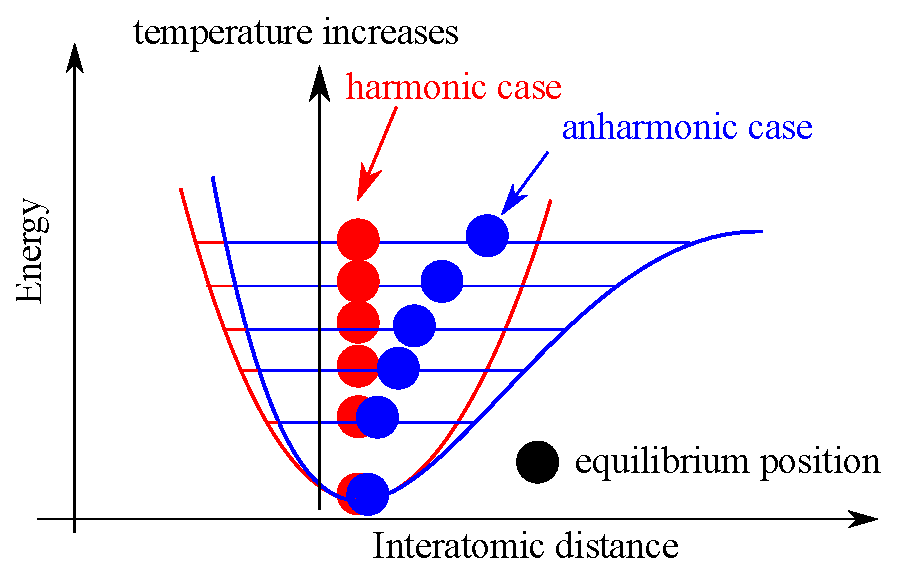
\includegraphics[width=0.8\linewidth]{anh_exp.eps}%
\caption{Schematic illustration of the relation between asymmetric interatomic potential and thermal expansion. }
\label{fig:anh_exp}
\end{figure}

The thermal expansion is the expansion of a material's volume at finite temperature. As shown in \autoref{fig:anh_exp}, it is directly related to the asymmetry of the interatomic potential where the equilibrium position shifts towards the flatter side of the potential energy profile and stays far away from the steeper side as the temperature increases. Below we will see how we can include this anharmonic potential using an approximation. The TEC $\alpha(T)$ is defined through the following formula: 
\begin{equation}
\alpha(T)=\frac{1}{a_0(T)}\frac{da_0(T)}{dT},
\end{equation}
where $T$ is the temperature, $a_0(T)$ is the equilibrium lattice parameter corresponding to the minimum of the Helmholtz free energy.

In order to describe the thermal expansion within DFT, one needs to go beyond the harmonic approximation that is used to calculate the phonon frequency as we discussed in \autoref{chap:3}. The harmonic approximation gives infinite thermal conductivity, infinite phonon lifetimes and temperature-independent vibrational and elastic properties, which contradict to the experiment. The quasi-harmonic approximation (QHA) \cite{QHA1,QHA2,QHA3,Baroni39} is a way to include the approximated anharmonic effect through volume-dependent frequencies within the non-interacting phonons approximation. Although it is an implicit inclusion of anharmonic effect, its dominant role in the thermal properties, that is two orders of magnitude larger than explicit anharmonic effects, make sure it can correctly describe the thermal properties up to melting point. Beyond this temperature, anharmonic effect will become important. QHA has been applied to various compounds from semiconductors to metals and to earth materials under extreme conditions\cite{QHA1,Grabowski2009,Karki2000} . In \autoref{fig:qha_gra}, the applications of the QHA for graphite and graphene are shown. The agreement between experiment and QHA is good in a wide range of temperature up to 2000 K. Another interesting point is that the negative thermal expansion, where the $\alpha(T)$ is negative, is presented in both materials, especially, graphene keeps such a feature up to 2000 K. This is a common character of layered materials where layers are weakly bonded. The origin of this is related to the ZA mode in layered materials as discussed in \autoref{chap:3}. At low temperature, ZA mode will be excited and this out-of-plane vibration effectively shrinks the in-plane dimension of the materials and thus gives negative thermal expansion.

\begin{figure}[htbp!] 
\centering
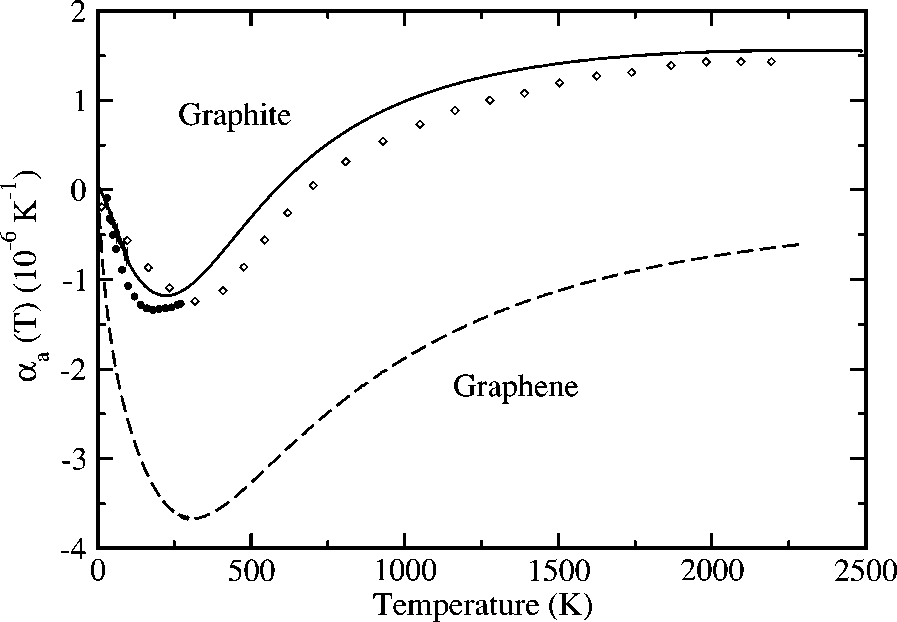
\includegraphics[width=0.8\linewidth]{qha_gra.png}%
\caption{ TEC of graphite and graphene calculated using QHA (solid line) and experimental result for graphite (points). Image source: \cite{QHA1} }
\label{fig:qha_gra}
\end{figure}

Equilibrium lattice constants at any temperature $a_0(T)$ are calculated by direct minimization of the Helmholtz free energy $F(a,T)$ with respect to its independent lattice vector, i.e. in this case, $\mathbf{a}$ and $\mathbf{b}$ for black P, and $\mathbf{a}$ for blue P. For the minimization process, $F(a,T)$ is obtained by fitting the discrete data points of $F({a_i,T})$ to the third-order Birch-Murnaghan equation of state, where $i$ is the label for different lattice constants or equivalently different strains. The $F({a_i,T})$ is constructed from $\omega^i_{\mathbf{q},j}$ and $E[a_i]$ through the following formula\cite{QHA0,QHA1}:
\begin{equation}\label{eq:free-enerji}
F({a_i,T}) = E[a_i]+\sum_{\mathbf{q},j}\frac{\hbar \omega^i_{\mathbf{q},j}}{2} +k_BT\sum_{\mathbf{q},j}\text{ln}\left( 1-\text{exp} \left[ -\frac{\hbar \omega^i_{\mathbf{q},j}}{k_BT} \right]\right).
\end{equation}
Here, $T$ is the temperature, $k_B$ is the Boltzmann constant, $E[a_i]$ is the DFT ground state energy. $\omega^i_{\mathbf{q},j}$ is the phonon frequency at the q point $\mathbf{q}$ with band index $j$. 
The sums  run over all q points and all bands of the whole Brillouin zone. Since the structural instabilities arise especially for the armchair direction when under compressive strain values larger than 4\%,  the calculation of phonon dispersions for both structures are performed under small strains, namely $\pm$ 2\%,  in order to evaluate $\omega^i_{\mathbf{q},j}$ and $E[a_i]$. Considering two independent lattice vectors \textbf{a} and \textbf{b} of black P two uniaxial strains are applied for these directions. While for blue P, only biaxial strain is applied to keep its hexagonal symmetry unchanged. The whole calculation process was carried out using the phonopy-qha script\cite{phonopy-qha}.

\subsection{Computational details}

\begin{footnotesize}
\begin{description}
\item[Simulation program:] VASP and Phonopy\cite{phonopy_code}
\item[Energy cut-off:] 500 eV
\item[Pseudopotentials:] PBE-GGA(PAW)
\item[k points ($Gamma$ centered):] 15$\times$11$\times$1 and 15$\times$15$\times$1 for black P and blue P, respectively 
\item[Vacuum:] 25~\AA
\item[Energy and force convergence criterion:] 10$^{-5}$ eV and 10$^{-7}$ eV/\AA, respectively
\item[Supercell for phonon calculation:] 7$\times$3$\times$1 and 5$\times$5$\times$1 for black P and blue P, respectively
\item[q points for phonon calculation:] 200$\times$200$\times$1
\end{description}
\end{footnotesize}

\subsection{Phonon modes and dispersion \label{sec:pho_phos}}

Different from a pure planar graphene, black P and blue P have a buckled non-planar structure due to the sp$^3$ hybridization, yet all three structures share the same hexagonal lattice base. Given an almost identical local environment in the unit cell, see \autoref{fig:phos_struc}, it is not surprising that blue P and black P having similar total energy. The only significant difference is the plane, marked as grey shown in \autoref{fig:phos_struc}, on which the system extends to form an infinite 2D crystal. Therefore, thermal expansion on these different planes are expected to be different and will carry insight and information on the different finite temperature properties. The primitive unit cell of black P is a rectangular lattice with a four-atom basis and a space group of $D_{2h}^7$, and that of blue P is a hexagonal lattice with a two-atom basis and a space group of  $D_{3d}^3$. Therefore, besides the three acoustic modes with the in-phase vibrations of atoms, there are nine and three optical modes for black P and blue P, respectively. 

\begin{figure}[htbp]
\centering
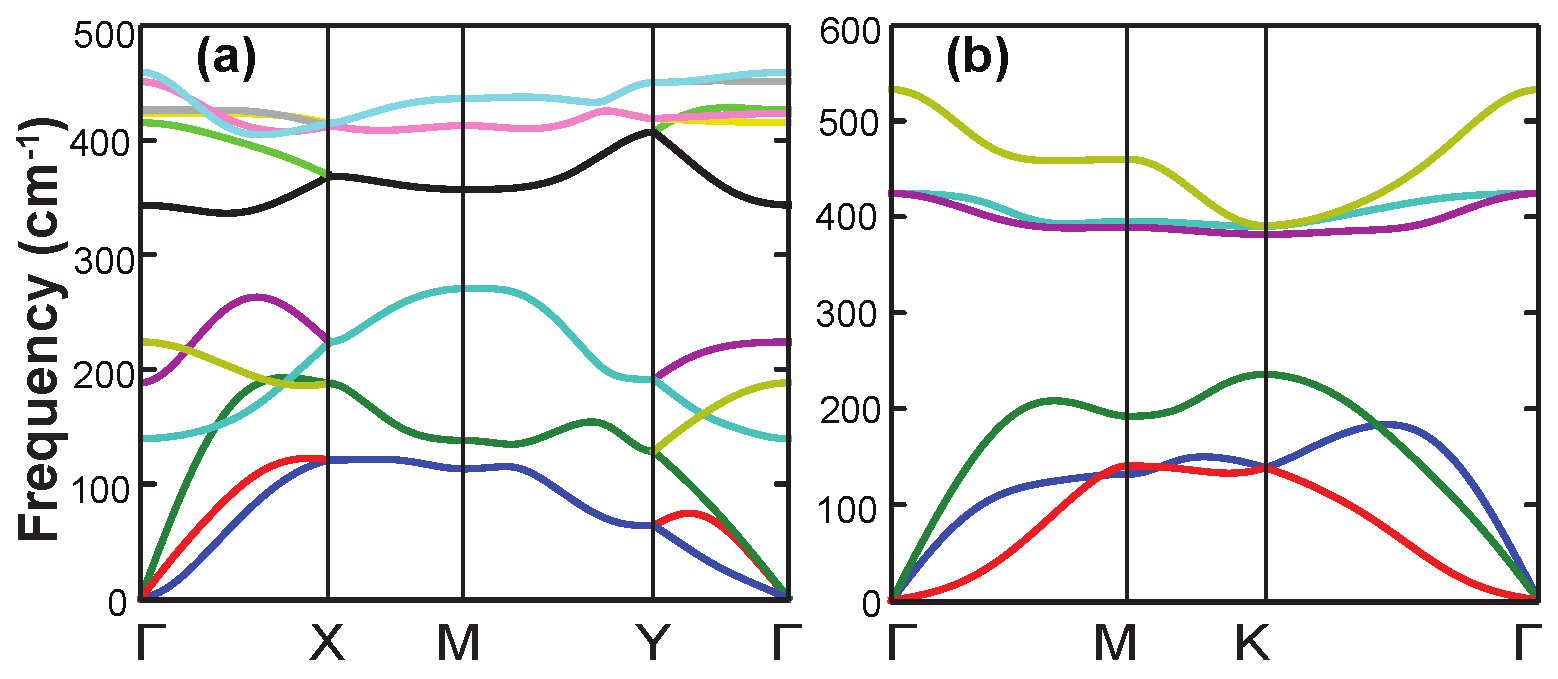
\includegraphics[width=0.8\linewidth]{phos_phon.eps}%
\caption{Calculated phonon dispersions for prinstine (a) black and (b) blue P.\label{phos_phon}}
\end{figure}

The calculated phonon dispersions along the high symmetric q lines corresponding to these modes are depicted in \autoref{phos_phon}(a) and (b) for both structures. Parallel with the previous calculations~\cite{phonon-blackP,phonon-blackP-1}, the calculated phonon dispersions are free from imaginary frequencies, which ensures the structural stability of the materials. The lowest acoustic mode ZA displays a $q^2$ relation as we discussed in \autoref{chap:3}.  The other two acoustic modes, LA and TA, still have a linear dependence with respect to the $q$ wavevector since the situation is the same here as in the bulk. The total frequency range of the phonon dispersion is larger by an amount of about 100 cm$^{-1}$ in blue P as compared to black P. 

\subsection{Temperature-dependent thermal properties}

The equilibrium lattice constants at zero K, $a_0$ and $b_0$ of black P and $a_0$ of blue P, are predicted as $a_0$ = 3.298 {\AA}, $b_0$=4.625 {\AA}, and  $a_0$ = 3.277 {\AA}, respectively,  in  good agreement with previously reported results ($a_0$ = 3.297 {\AA}, $b_0$=4.640 {\AA} for black P\cite{fei,deniz3}, and  $a_0$ = 3.330 {\AA} for blue P\cite{Zhu2014}). 
The expansion of these lattice parameters due to zero-point vibration is around 0.2\% at 0 K, which is smaller than that of other well-known 2D materials like graphene and $h$-BN, but it is comparable with that of MoS$_2$ and MoSe$_2$. This result is reasonable due to the difference in the maximum phonon frequency between these materials: that of graphene and $h$-BN is around 1600 cm$^{-1}$ and that of MoS$_2$, MoSe$_2$, black P and $a_0$ of blue P is around 600 cm$^{-1}$. 

\begin{figure}[htbp]
\centering
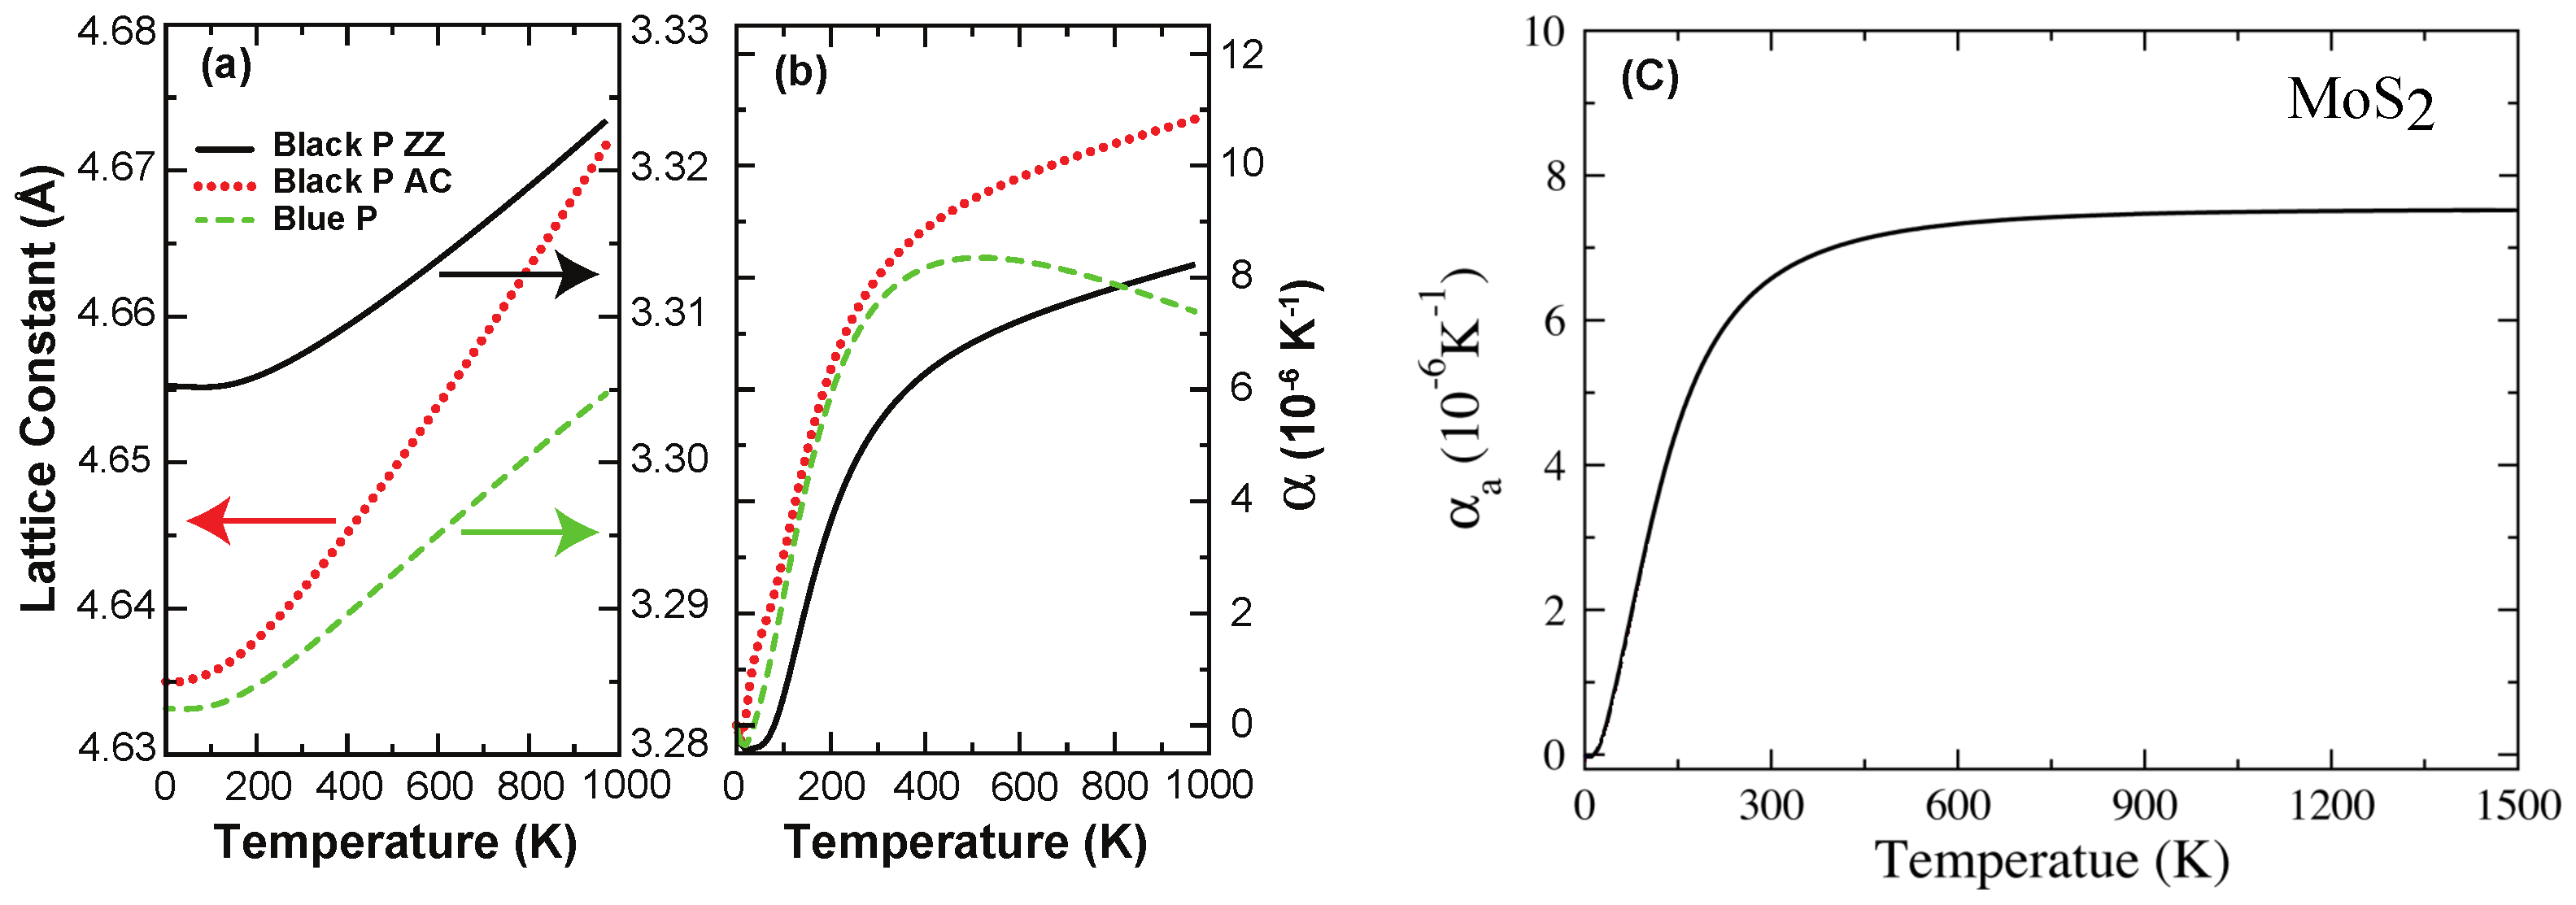
\includegraphics[width=\linewidth]{expan_T.eps}%
\caption{(a) Lattice constants and (b) TEC of black P and blue P as a function of temperature.  Here, ZZ and AC are denoted for the zigzag and armchair directions, respectively. (c) TEC of monolayer MoS$_2$ for comparison from Ref. \cite{QHA3}.\label{fig:tec}}
\end{figure}

The temperature dependence of the lattice constants $a_0(T)$, $b_0(T)$ and TEC $\alpha(T)$ of both structures are shown in \autoref{fig:tec}. The anisotropic nature of the structure of black P leads to different lattice constant expansion rates. A faster thermal expansion along the armchair direction (i.e. $\mathbf{b}$) is found, see \autoref{fig:tec}(a). While a small negative TEC appears for all structures in all directions at temperatures lower than 100 K, black P along the zigzag direction has a more apparent negative expansion.  The lattice constant of both phases varies linearly when T $>$ 200 K, see \autoref{fig:tec}(a). The TEC increases rapidly with temperature  up to 300 K.  After that, all TECs changes slowly with temperature starting from around 400 K in agreement with predictions for 2D-TMDs~\cite{QHA2,QHA3}, for example see \autoref{fig:tec}(c) for monolayer MoS$_2$.
Different from MoS$_2$, we do not observe any saturation of the TEC for black P at high temperatures.  While black P expands at most 0.02 {\AA} along the zigzag direction as T approaches 1000 K, it expands 0.04 {\AA} along the armchair direction. As is clear from \autoref{fig:phos_struc}, a uniaxal expansion along the armchair direction may result in a structural phase transition from black P to blue P because of the similar hexagonal arrangement of P atoms\cite{negative-pos}. 

\begin{figure}[htbp]
\centering
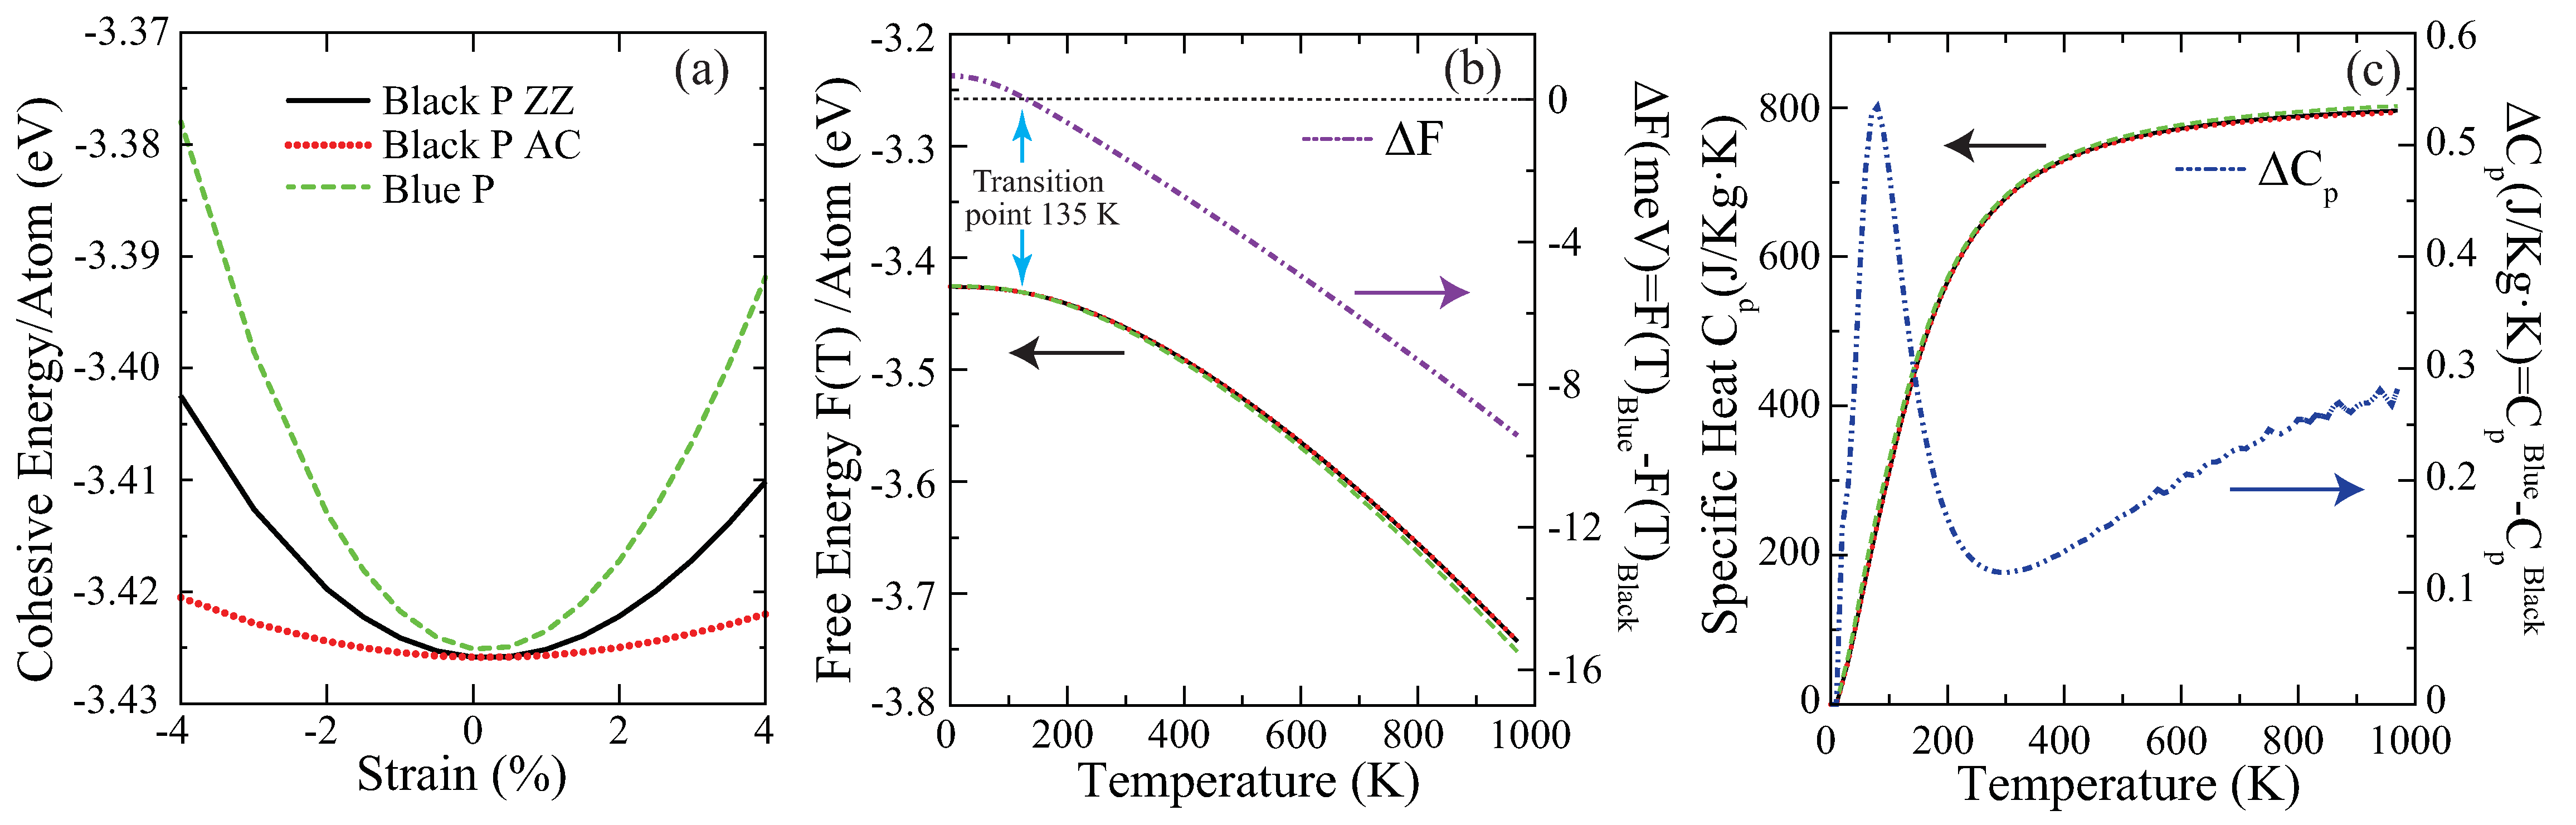
\includegraphics[width=\linewidth]{freeE_T.eps}%
\caption[Thermal properties variations of phosphorene with temperature]{(a) Cohesive energy, including zero point energy, as a function of applied strain at $T$ = 0 K and (b) Helmholtz free energy ($F(T)$) as a function of temperature.  Here, ZZ and AC are used for the zigzag and armchair directions, respectively. $\Delta F(T)$ is the difference between $F(T)$ of black P and blue P. The blue arrow  (b) denotes the transition point, after which blue P becomes thermodynamically more stable over black P.  The specific heat at constant pressure ($C_p$) and the difference ($\Delta C_p$) between $C_p$ of black P and blue P are shown in (c).  \label{energies_data}}
\end{figure}

In \autoref{energies_data}, the variation of the cohesive energy as a function of strain at 0 K (a) and the variation of the Helmholtz free energy (F(T)) as a function of temperature (b) are presented. In \autoref{energies_data}(b), 
we also show $\Delta F(T)$ which is defined as $\Delta F(T)$=$F_{blue P}(T)$ - $F_{black P}(T)$. Here, $F_{blue P}(T)$ and $F_{black P}(T)$ are the Helmholtz free energy of black P and blue P, respectively. As the zero-point energy continuously decreases with strain from minus to plus, the variation of the zero-point energy results in an asymmetric behaviour in cohesive energy with strain. In addition, the curvature of this total energy gives the in-plane stiffness of the material as a measure of the response to mechanical deformation. It is clear that blue P is a stiffer material as compared to black P.  Moreover, the deformation along the zigzag direction of black P is harder than that along the armchair direction at 0 K, and this is consistent with the finite temperature behaviour as we concluded from the previous section in connection with \autoref{fig:tec}(a). 

The $F(T)$ decreases as temperature increases due to the entropy term (the last term in \autoref{eq:free-enerji}). Inclusion of the zero-point energy gives rise to a slightly higher ground state energy for blue P over black P since its optical phonon modes have larger frequencies. However, as temperature increases, a crossing of the free energy curves around 135 K occurs, which makes the blue P energetically more favorable at high temperatures, see \autoref{energies_data}(b). The free energy difference between the two phases is of the order of 4 meV at room temperature, meaning that the two phases can coexist. In addition, it is possible to observe a phase transition driven by temperature from black P to blue P or visa verse at T=135 K. 

In \autoref{energies_data}(c), we present constant pressure heat capacity, $C_p$, results for both structures, which is generally a few percent different from constant volume heat capacity in similar structures\cite{QHA1}. The $C_p$ difference ($\Delta C_p$) between two phases is significantly small for the whole temperature range as represented with a blue dash-dot line in \autoref{energies_data}(c), which shows essentially very similar Debye temperature for these two different phases.  At high temperatures, C$_p$ approaches its classical value of 12 $k_B$.  When T=300 K, C$_p$ already reaches about 80 $\%$ of its classical value, meaning that most of the phonon modes are activated at this temperature. 

\subsection{Summary}

In summary, we systematically investigated the lattice thermal properties of black and blue P. Similar to its electronic properties, black P has direction dependent mechanical and thermal properties. The calculated TEC demonstrates that a much larger expansion along the armchair direction with temperature is observed for black P. While black P is thermodynamically more stable than blue P, the latter becomes more stable when T $>$ 135 K. Yet their free energy difference is small due to their structural similarities. It is possible to observe a structural phase transition from black P to blue P by increasing the temperature beyond 135 K, and therefore the coexistence of these two phases is possible. 

\section[Piezoelectric properties of 2D-TMDs and 2D-TMDOs]{Piezoelectric properties of 2D-TMDs and 2D-TMDOs \footcite[This work is published:][]{Menderes2015} \label{piezo_mx2}}

\subsection{Introduction}

We have seen the general properties of 2D-TMDs in \autoref{chap:1} and the vibrational and electronic properties of one member: 2D-MoS$_2$ in \autoref{chap:3}. When the S atom is replaced with O, TMDs become TMDOs, whose monolayers have similar properties as 2D-TMDs. Although 2D-TMDOs are proven to be stable, they have not been synthesised yet. Sharing similar electronic structure, 2D-TMDs and 2D-TMDOs already promise various potential applications, such as nanoelectronic and nanophotonic devices owe to their direct finite band gaps\cite{Jariwala2014,Wang2012}. In addition to these exciting applications, 2D-TMDs, in the noncentrosymmetric 2H crystal structure with $D_{3h}$ symmetry, have also been shown to have remarkable piezoelectric properties that can then be used in pressure sensors, transducers, high voltage generators, energy harvesters, energy conversion and piezotronic applications. Many layered materials have a centrosymmetry which suppresses piezoelectricity. However, this symmetry will be broken at the monolayer level, and then piezoelectricity is recovered. For example, graphene preserves centrosymmetry as in graphite, or inversion symmetry, due to its non-polar nature, thus it does not display piezoelectricity. Whereas, 2D-BN and 2D-TMDs break such symmetry and become noncentrosymmetric systems where piezoelectric effects can manifest themselves. 

\citet{Duerloo2012} calculated the piezoelectric properties of a single layer of BN, MoS$_2$, MoSe$_2$, MoTe$_2$, WS$_2$, WSe$_2$, and WTe$_2$ by using first-principles calculations. They reported that piezoelectricity of the 2D-TMDC monolayers in the H phase are comparable or even better than that of conventional bulk piezoelectric materials. \citet{Zhu2015} reported 
experimental evidence of piezoelectricity in free-standing MoS$_2$ and they found that this material exhibits piezoelectricity for an odd number of layers in which case inversion symmetry is broken. Their measured piezoelectric coefficient is 2.9$\times$10$^{-10}$ C/m, which agrees well with previous theoretical calculations\cite{Duerloo2012}.  Similarly, by using DFT based theoretical calculations, it has been predicted that group IIIA monodichalcogenides, namely GaS, GaSe and InSe, have piezoelectric stress coefficients of 1.34$\times$10$^{-10}$, 1.34$\times$10$^{-10}$ and 1.47$\times$10$^{-10}$ C/m, respectively\cite{Li2015a}.  In addition, reducing the dimensionality has been shown to enhance piezoelectricity in ZnO\cite{Xiang2006}. These studies indicate that TMDs are promising candidates as low dimensional piezoelectric materials. 

Since previous calculations and experiments were only focused on Mo and W based TMDs, the potential of other 2D-TMDs and 2D-TMDOs for piezoelectric device applications have remained an open question so far. To reveal such potential, first principles calculations are performed in order to systematically investigate the piezoelectric properties of single layer 2H-MX$_2$ compounds, where M= Cr,  Mo, W, Ti, Zr, Hf, Sn and X=O, S, Se, Te.  Lattice parameters, atomic positions, electronic band-gap values, elastic stiffness constants ($C_{11}$ and $C_{12}$), Young modulus ($Y$), Poisson's ratios ($\nu$), piezoelectric stress coefficients ($e_{11}$) and piezoelectric strain coefficients ($d_{11}$) are calculated. 

\subsection{Piezoelectric constants}

Piezoelectricity is the ability of some materials to generate an internal electric field in response to applied mechanical stress. Two types of piezoelectric phenomena can be observed for piezoelectric materials: 1) direct piezoelectric effect: separation of opposite charge due to stress and 2) converse piezoelectric effect: occurrences of stress and strain under external electric field. In \autoref{fig:piezo}, the mechanism of direct piezoelectric effect is shown. 

\begin{figure}[htbp]
\centering
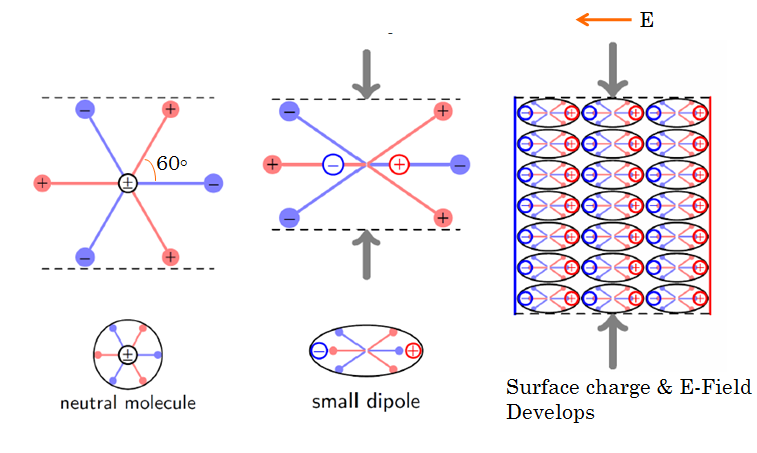
\includegraphics[width=0.8\linewidth]{piezo.png}%
\caption{Mechanism of direct piezoelectric effect\label{fig:piezo}. Image source: \cite{piezo_fig}}
\end{figure}

To investigate the piezoelectric properties, we follow the same theoretical approach as Ref. \cite{Duerloo2012}. The piezoelectric tensor\cite{baroni,PhysRevB.72.035105}, $e_{ij}$, can be defined in terms of the induced polarization in the  direction $i$ due to a strain ($\varepsilon_{j}$) change along the direction $j$ as follows
\begin{equation}
e_{ij}=\partial P_{i}/\partial\varepsilon_{j}=\partial P_{i}/\partial\varepsilon_{j}\mid_u+\sum_k (\partial P_{i}/\partial u_{ik})(\partial u_{ik}/\partial\varepsilon_{j}). \label{eq:equ1}
\end{equation}
where $P_i$ is the induced polarization along the direction $i$ as a result of an applied strain $\varepsilon_{j}$ along the direction $j$. 
The $P_i$ is calculated using the Berry Phase approach\cite{vanderbilt2000} as implemented in the VASP package with applied uniform strain, ranging from 1 \% to -1 \% in steps of 0.5 \%, along the armchair side of the rectangular cell. At this point, in order to apply strain in a desired direction, the hexagonal primitive cell structure of each material is transformed to a tetragonal one composed of two hexagonal primitive cells\cite{Duerloo2012}, see \autoref{fig:mx2_str}. The first term in \autoref{eq:equ1} is the clamped-ion or homogeneous strain contribution to the piezoelectric tensor and it mainly arises from the electronic contribution. The second term represents the contribution from the internal relaxation of ions. Here, $u_{ik}$ is the fractional coordinate of the $k^{th}$ atom along the $i$ direction of the unit cell. 

Since TMDs and TMDOs compounds have a non-centrosymmetric crystal structure, the inclusion of internal relaxation becomes essential in order to obtain realistic piezoelectric properties. In addition, it is clear that the relaxed-ion piezoelectric coefficients are experimentally relevant quantities that can be measured. From the theoretical point of view, since the relaxed-ion piezoelectric coefficients include both electronic and relaxation effects, the calculation of the clamped-ion piezoelectric coefficients helps to separate the electronic and relaxation contributions from the relaxed-ion piezoelectric coefficients. The number of independent piezoelectric tensor coefficients is deduced from the symmetry of the crystal. For TMDs and TMDOs, we only need to calculate the $e_{11}$ component of the piezoelectric stress tensor. $e_{11}$ relates in-plane strain to in-plane electrical polarization. The piezoelectric coefficient $e_{31}$ is zero due to the presence of an inversion centre between the two layers of chalcogenides. However, it is found to be non-zero for the unsymmetrical H and F co-decorated graphene\cite{Ong2013,KIM201462}. 

The corresponding piezoelectric strain tensor ($d_{11}$) of each material is predicted from the following relation\cite{Duerloo2012}:
\begin{equation}\label{eq:d11}
                d_{11}= e_{11}/( C_{11} - C_{12} ).
\end{equation}
For each applied strain, the ions are kept in their strained positions or allowed to relax to their new equilibrium positions, and consequently the clamped-ion or relaxed-ion piezoelectric properties are calculated, respectively.

\begin{figure}[htbp]
\centering
	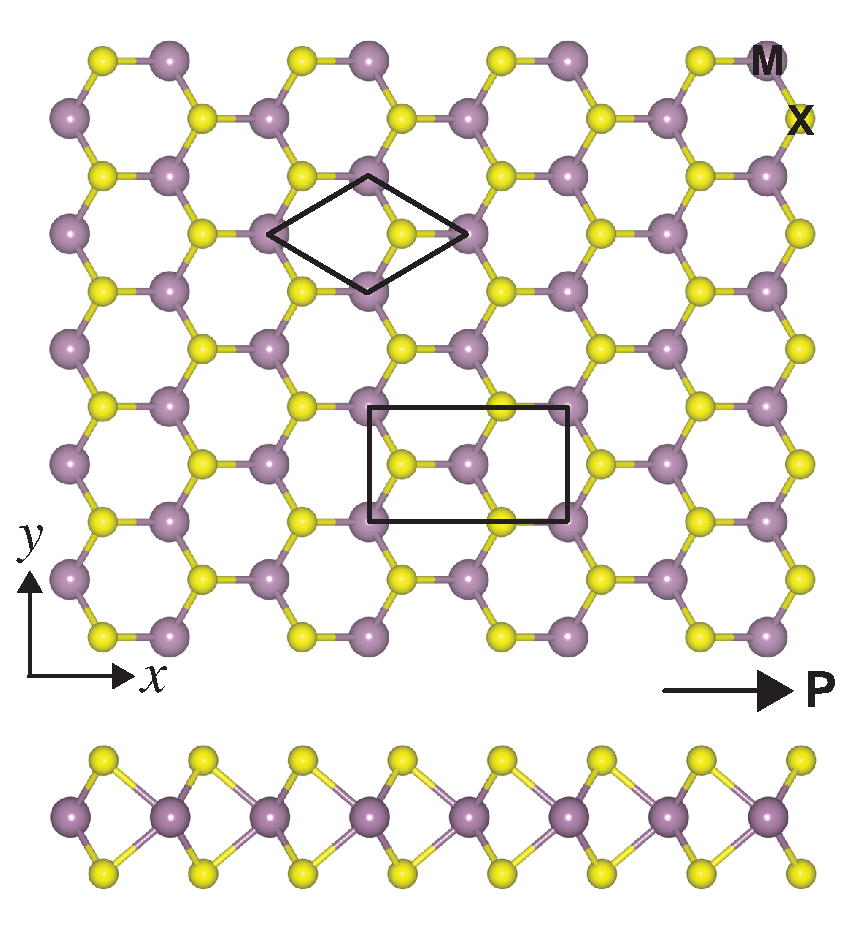
\includegraphics[width=0.5\linewidth]{mx2_str.eps}
	\caption{Top and side views of MX$_2$ where M= Cr,  Mo, W, Ti, Zr, Hf, Sn and X=O, S, Se, Te. P denotes the direction of the polarization. Piezoelectric calculations are done in a rectangular cell. \label{fig:mx2_str}}
\end{figure}

\subsection{Computational details}
\begin{footnotesize}
\begin{description}
\item[Simulation program:] VASP
\item[Energy cut-off:] 600 eV
\item[Pseudopotentials:] PBE-GGA(PAW), HSE06
\item[k points ($Gamma$ centered):] 26$\times$26$\times$1
\item[Vacuum:] 15~\AA
\item[Energy and force convergence criterion:] 10$^{-3}$ eV and 10$^{-7}$ eV/\AA, respectively
\item[strain applied:] 1\% to -1\% in steps of 0.5\%
\item[stress and force:] finite displacement method
\item[polarization:] Berry Phase expression \cite{vanderbilt2000} in VASP
\end{description}
\end{footnotesize}

\subsection{Accurate band gaps from HSE06 hybrid functional}

It is mandatory that a piezoelectric material has to be an insulator or semiconductor with a sufficiently wide band gap to avoid current leakage. Thus, we first calculate the electronic properties of twenty eight single layer MX$_2$ compounds, where M= Cr,  Mo, W, Ti, Zr, Hf, Sn and X=O, S, Se, Te. We discard the metallic structures, namely SnSe$_2$, SnTe$_2$, and TiTe$_2$. Actually, G$_0$W$_0$ calculations predicted that 2H-TiTe$_2$ is a small band gap semiconductor material\cite{Rasmussen2015}. Since semi-local functionals are used in the Berry's phase calculations, 2H-TiTe$_2$ is excluded. For electronic structure calculations, we also applied the HSE06 hybrid functionals in order to obtain realistic electronic band gap values for TMDs and TMDOs. \autoref{fig:bandgaps} shows the calculated PBE-GGA and HSE06 band gap values E$_{gap}$. The materials, except Cr, Mo, and W based TMDs, have indirect band gaps and the predicted values and trends are in good agreement with previous theoretical calculations\cite{Duerloo2012,Ataca2012,Guo2014a}. Generally, the band gap increases when moving upwards in the chalcogens family from Te to S and with increasing atomic number in the transition metals. However, the latter trend is only partially valid when the compounds with O are included. The difference is that within the same row of the transition metals, TMDOs with a larger atomic number tend to have smaller band gaps which is in contrast to the TMDs case.

\begin{figure}[htbp]
\centering
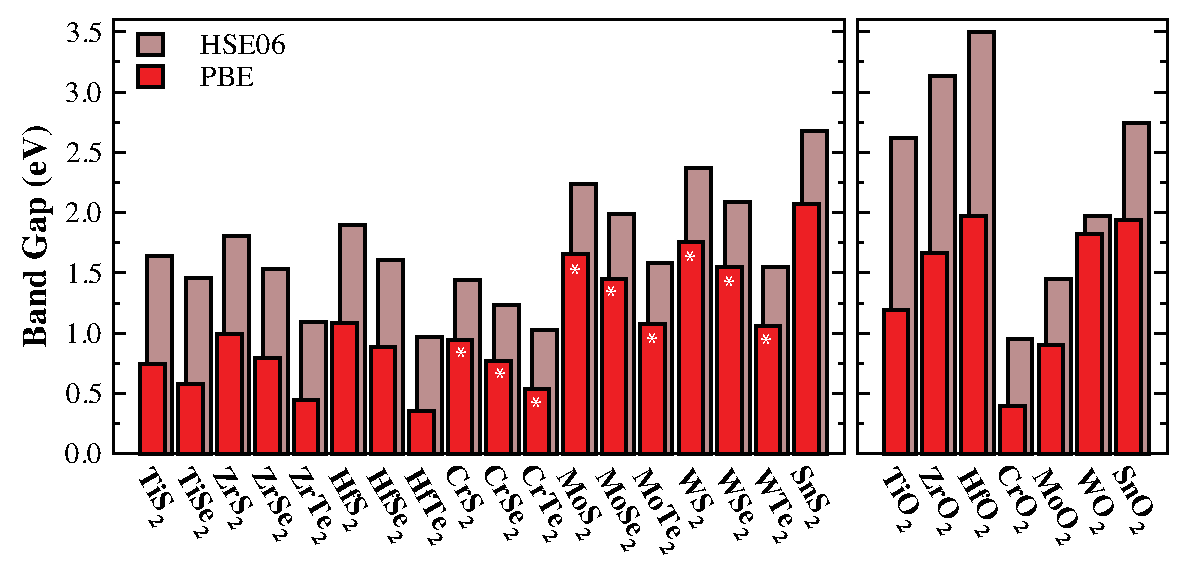
\includegraphics[width=0.8\linewidth]{bandgaps.eps}
\caption{\label{fig:bandgaps}The calculated PBE-GGA and HSE06 E$_{gap}$ values for TMDs and TMDOs. Here, the white * sign indicates that it is a direct band gap material.}
\end{figure}

\subsection{Elastic constants}\label{elastic}

\begin{table}[htbp]
\centering
\caption{\label{tab:elastic}Calculated clamped and relaxed-ion elastic constants (in units of N/m), Young modulus Y (in units of N/m) and Poisson's ratio $\nu$.  }
\begin{tabularx}{\linewidth}{lXXXXsXXXX}
 \hline\hline
 Material& \multicolumn{4}{c}{Clamped Ion} && \multicolumn{4}{c}{Relaxed Ion}\\\cline{2-5}\cline{7-10}
 &  $C_{11}$ & $C_{12}$ & $Y$ & $\nu$ && $C_{11}$ & $C_{12}$ & $Y$ & $\nu$ \\\hline
TiS$_2$ & 100.3 &  34.2 &  88.6 & 0.34 &&  89.9 & 28.6 &  80.8 & 0.32\\
TiSe$_2$ & 84.8 &  29.3 &  74.7 & 0.35 &&  74.4 & 24.4 &  66.4 & 0.33\\
ZrS$_2$ &  96.3 &  37.7 &  81.5 & 0.39 &&  84.2 & 31.8 &  72.2 & 0.38\\
ZrSe$_2$ &  83.3 &  31.0 &  71.8 & 0.37 &&  71.4 & 26.0 &  61.9 & 0.36\\
ZrTe$_2$ &  66.2 &  22.8 &  58.35 & 0.34 &&  53.1 & 18.6 &  46.6 & 0.35\\
HfS$_2$ & 104.4 &  39.1 &  89.8 & 0.37 &&  92.8 & 33.8 &  80.5 & 0.36\\
HfSe$_2$&  89.7 &  32.2 &  78.1 & 0.36 &&  78.8 & 27.8 &  69.0 & 0.35 \\
HfTe$_2$&  71.0 &  23.5 &  63.2 & 0.33 &&  59.3 & 19.7 &  52.8 & 0.33 \\
CrS$_2$ & 136.9 &  42.6 & 123.6 & 0.31 && 120.6 & 32.3 & 111.9 & 0.27\\
CrSe$_2$& 111.3 &  37.5 &  98.7 & 0.34 &&  96.6 & 28.9 &  87.9 & 0.30\\
CrTe$_2$&  86.5 &  32.7 &  74.1 & 0.38 &&  73.0 & 25.8 &  63.9 & 0.30\\
MoS$_2$ & 157.2 &  50.1 & 141.2 & 0.32 && 132.7 & 33.0 & 124.5 & 0.25\\
MoSe$_2$& 133.2 &  40.8 & 120.7 & 0.31 && 106.9 & 25.6 & 100.8 & 0.24\\
MoTe$_2$& 106.3 &  32.8 &  96.2 & 0.31 &&  84.1 & 19.8 &  79.4 & 0.24\\
WS$_2$  & 174.7 &  51.9 & 159.3 & 0.30 && 146.5 & 31.8 & 139.6 & 0.22\\
WSe$_2$ & 147.4 &  41.1 & 135.9 & 0.28 && 102.4 & 23.1 & 115.9 & 0.23\\
WTe$_2$ & 115.4 &  31.6 & 106.8 & 0.27 &&  89.2 & 15.7 &  86.4 & 0.18\\
SnS$_2$ &  92.8 &  23.1 &  87.1 & 0.25 &&  91.0 & 22.2 &  85.6 & 0.24\\
TiO$_2$ & 178.9 &  80.9 & 142.3 & 0.45 && 173.7 & 75.7 & 141.7 & 0.44\\
ZrO$_2$ & 163.5 &  83.0 & 121.5 & 0.51 && 157.4 & 77.5 & 119.2 & 0.49\\
HfO$_2$ & 181.7 &  86.7 & 140.3 & 0.48 && 174.2 & 81.5 & 136.1 & 0.47\\
CrO$_2$ & 233.8 &  87.4 & 201.1 & 0.37 && 218.6 & 74.4 & 193.3 & 0.34\\
MoO$_2$ & 253.3 & 104.0 & 210.6 & 0.41 && 230.2 & 84.5 & 199.2 & 0.37\\
WO$_2$  & 286.2 & 109.0 & 244.7 & 0.38 && 261.2 & 87.8 & 231.7 & 0.34\\
SnO$_2$ & 165.7 &  52.4 & 149.1 & 0.32 && 160.2 & 53.3 & 142.5 & 0.33\\
\hline\hline
\end{tabularx}
\end{table}

As previously mentioned, we need to calculate the elastic constants in order to obtain the piezoelectric strain, $d_{11}$ coefficients, see \autoref{eq:d11}. Therefore, the relaxed-ion and clamped-ion elastic stiffness coefficients (C$_{11}$ and C$_{12}$), Young modulus (Y= (C$_{11}^2$-C$_{12}^2$)/C$_{11}$) and Poisson's ratios ($\nu$=C$_{12}$/C$_{11}$ ) for all 2D-TMDC and 2D-TMDO materials considered in this study are obtained and are listed in \autoref{tab:elastic}. Our results are in good agreement with available data\cite{Peng2013,Kang2013,Duerloo2012,Cooper2013}. The first observation from \autoref{tab:elastic} is that C$_{11}$, C$_{12}$ and Y decrease with increasing row number of the chalcogenide atom. Except Zr, in each chalcogenide group, the MX$_2$ monolayer becomes stiffer with increase of the row number of the metal atom. Structures considered in this study are found to be less stiff when compared to graphene (Y=341 N/m)\cite{QHA2} and single layer $h$-BN (Y=275.9 N/m)\cite{QHA2}. Also it should be noticed that the calculated elastic constants are positive and satisfy the Born stability criteria for crystals having hexagonal symmetry\cite{nye1985physical,Born1998}.  Note that the relaxed-ion elastic constants, i.e. C$_{11}$ and C$_{12}$, are always smaller than the clamped-ion ones since the internal relaxation of ions allows to release some of the stress in the former, see \autoref{tab:elastic}.

\subsection{Piezoelectric stress/strain coefficients}\label{piezo}

\begin{figure}[htbp]
\centering
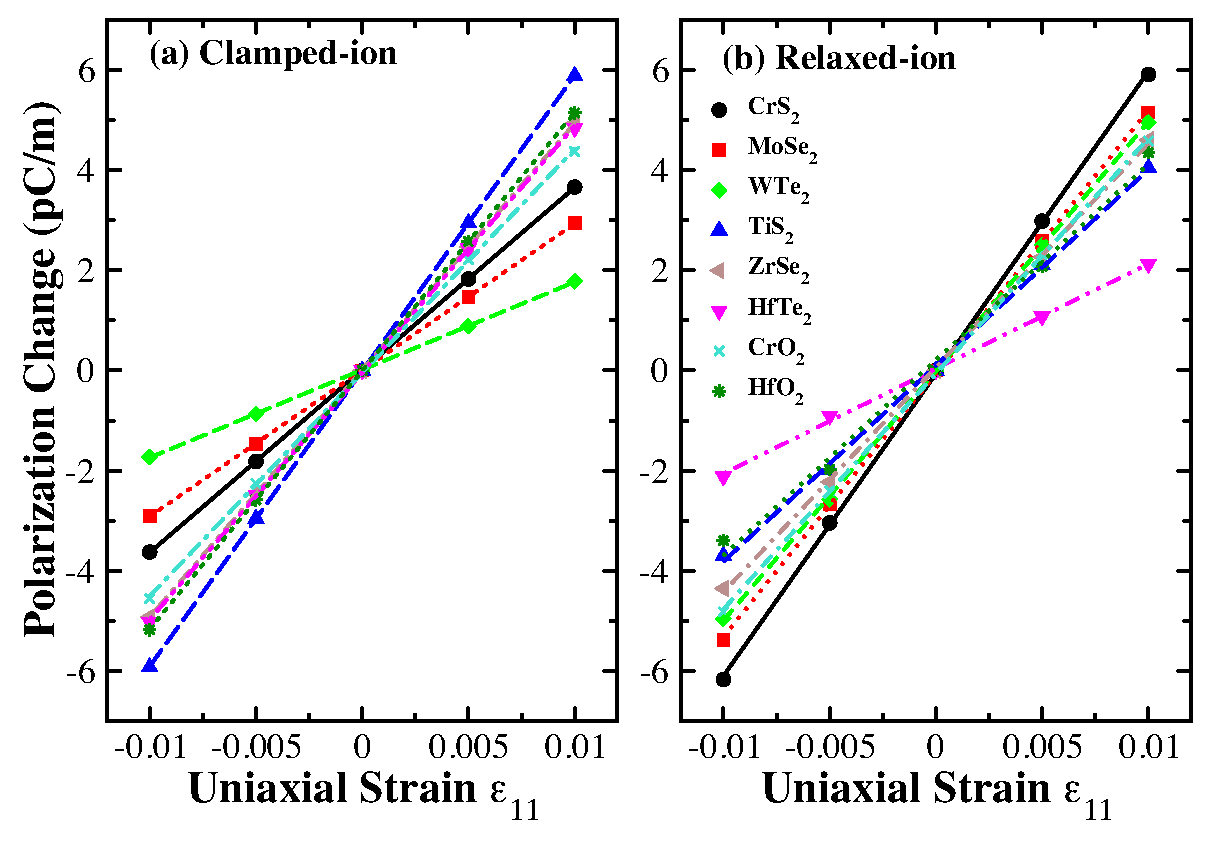
\includegraphics[width=0.8\linewidth]{polariz.eps}
\caption{\label{fig:polariz} (a) Clamped-ion and (b) relaxed-ion polarization change under applied uniaxial strain ($\varepsilon_{11}$) along the $x$ direction for the selected 2D-TMDs and 2D-TMDOs structures. Piezoelectric coefficient is determined from the slope of the curves.}
\end{figure}

\begin{figure}[t]
\centering
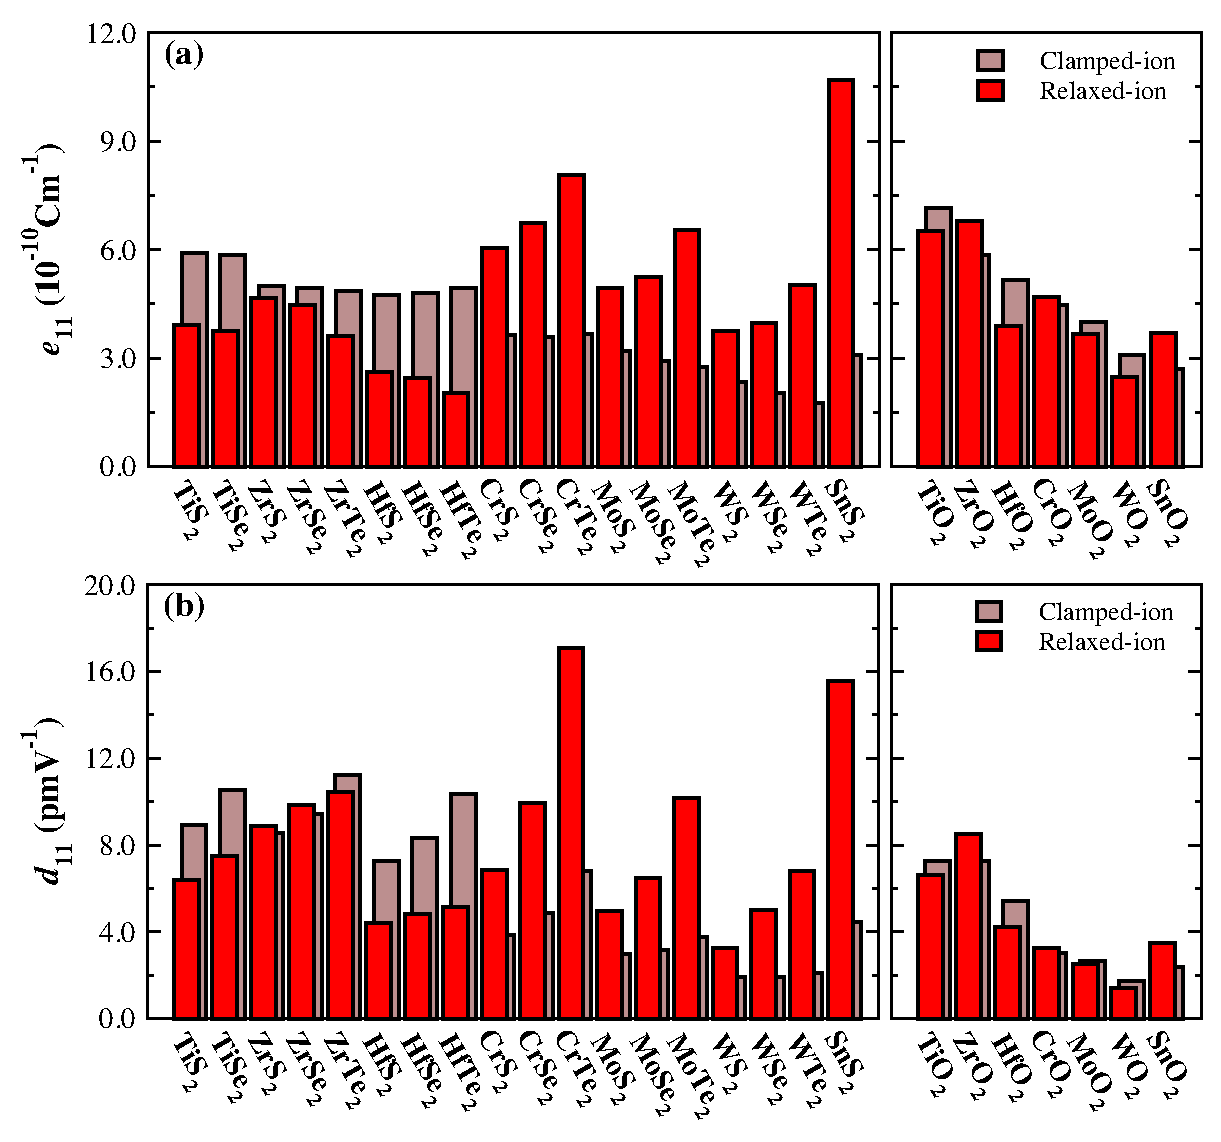
\includegraphics[width=0.8\linewidth]{piezo_res.eps}
\caption{\label{fig:piezo_res}The calculated clamped and relaxed-ion (a) piezoelectric stress ($e_{11}$)  and (b) piezoelectric strain ($d_{11}$) coefficients.}
\end{figure}

Piezoelectric coefficients ($e_{11}$) are derived from the slope of the polarization change in \autoref{fig:polariz}) with applied uniform strain, ranging from 0.01 \% to -0.01 \% in steps of 0.005 \%, along the armchair side of the rectangular cell via Berry's Phase approximation\cite{vanderbilt2000}. The clamped-ion and relaxed-ion $d_{11}$ coefficients are obtained by using the calculated $e_{11}$ coefficients, and the elastic constants ($C_{11}$ and $C_{12}$) via \autoref{eq:d11}. \autoref{fig:piezo_res} shows the calculated $e_{11}$ and $d_{11}$ coefficients for both TMDs and TMDOs. The materials are ordered along the $x$-axis by considering the period and group number of the transition metal element in the periodic table. The predicted relaxed-ion $e_{11}$ and $d_{11}$ coefficients are consistent with the available reference data\cite{Duerloo2012,crs2}, see results for Cr, Mo and W based TMDs, which are comparable with the piezoelectric properties of single layer and bulk $h$-BN\cite{Duerloo2012,km-2009,km-2011a,km-2011b}. In addition, the relaxed-ion $e_{11}$ coefficient of single layer MoS$_{2}$ (4.91$\times$10$^{-10}$ C/m) is comparable with the experimentally measured piezoelectric coefficient of 2.90$\times$10$^{-10}$ C/m\cite{Zhu2015} and agrees  well  with the reported value of 3.64$\times$10$^{-10}$ C/m.\cite{Duerloo2012}. In addition, the trends found for the $e_{11}$ and $d_{11}$ coefficients of Mo and W based TMDs are consistent with those found in Ref.\cite{Duerloo2012}. The difference between our calculated piezoelectric coefficients and previous calculations is likely due to the use of different pseudopotentials, small differences in elastic constants, and other computational parameters (for instance $k$-mesh).

SnS$_2$ has the highest $e_{11}$ coefficient for the relaxed-ion (10.7$\times$10$^{-10}$ C/m) calculation. WO$_2$ has the smallest relaxed-ion piezoelectric stress coefficient (2.49$\times$10$^{-10}$ C/m) among TMDOs and WTe$_2$ has the smallest clamped-ion piezoelectric stress coefficient (1.75$\times$10$^{-10}$ C/m). From \autoref{fig:piezo_res}, we predict several  periodic trends in clamped-ion $e_{11}$ and $d_{11}$ coefficients for TMDC and TMDO monolayers. The clamped-ion $e_{11}$ coefficients of TMDs usually increase when moving from right to left in the periodic table (i.e., from CrX$_{2}$ to TiX$_{2}$) and upward in an individual group of both transition metal and chalcogen atoms.  This trend is nearly the same for TMDOs. However, for TMDs, the trend (i.e., the increase in the calculated clamped-ion $e_{11}$ coefficients when moving upward in the group of chalcogen elements) becomes reversed for the relaxed-ion calculations of group VIB elements as clearly seen in \autoref{fig:piezo_res}(a). 
The clamped and relaxed ion $d_{11}$ coefficients increase when moving downward in the group of chalcogen elements (i.e. from S to Te) in each metal group.  This trend can be correlated to the polarizability of chalcogen atoms since the atoms are easily polarized when going downward in a specific group of the periodic table.  We notice that the chalcogenide atoms have a much larger impact on the $d_{11}$ coefficients as compared to the metal atoms.  Especially in group VI, the $d_{11}$ coefficient is maximized if one uses a smaller metal atom and a larger chalcogen atom. In group IVB, Zr does not exhibit the same trend that is found for the group VIB elements. This is partially because the C$_{11}$ elastic constant of Zr based TMDs for a particular chalcogen atom is smaller that that of Ti and Hf based TMDs. Since TMDOs pose larger elastic constants, they usually have smaller $d_{11}$ coefficients as compared to TMDs. In other words, the stronger the material the smaller the $d_{11}$ coefficient.  

Among the group VIB elements (i.e., Cr, Mo and W), Cr based TMDs and TMDOs are found to have much better piezoelectric properties in each chalcogenide group and CrTe$_2$ possesses the largest relaxed-ion  $e_{11}$ (8.06$\times$10$^{-10}$ C/m) and $d_{11}$ (17.1 pm/V) coefficients. On the other hand, the relaxed-ion $e_{11}$ and $d_{11}$ coefficients of SnS$_{2}$ are  almost the same as those of CrTe$_2$. The predicted relaxed-ion $e_{11}$ values are much larger than the values previously predicted for surface decorated graphene structures\cite{Ong2012}. Furthermore, when the piezoelectric coefficients of the extensively used bulk piezoelectric materials, namely 2.3 pm/V for  $\alpha$-quartz\cite{Bechmann1958}, 3.1 pm/V for wurtzite GaN\cite{Lueng2000} and 5.1 pm/V for AlN\cite{Lueng2000}, are considered, we predict that TMDs and TMDOs have comparable or even larger relaxed-ion piezoelectric coefficients.

\subsection{Importance of internal relaxation}

It is  essential to discuss the effect of the internal relaxation on the piezoelectric properties of TMDs and TMDOs. Relaxing the ion positions after applying strain significantly reduces (increases) the polarization of the  Ti, Zr and Hf (Cr, Mo and W) based TMDs. As a result, the clamped-ion piezoelectric coefficients of the Ti, Zr and Hf (Cr, Mo and W) based TMDs monolayers are much larger (smaller) than that of the relaxed-ion coefficients. This means that the electronic contribution, i.e. the first term in \autoref{eq:equ1}, and strain contribution, i.e. the second term in \autoref{eq:equ1}, have opposite (the same) sign for the  Ti, Zr and Hf (Cr, Mo and W) based TMDs.  The calculated elastic constants suggest that Ti, Zr and Hf based TMDs are more brittle materials that are expected to exhibit larger response to an applied strain, thereby giving rise to higher clamped-ion piezoelectric constants.  For TMDOs, the contribution of internal relaxation to the $e_{11}$ coefficient decreases when moving downward in an individual metal group. 
However, in each chalcogen group, the internal relaxation becomes  generally less important when going from Te to S. This can be attributed to the large strain-induced ionic motion in response to an applied strain. 
In other words, after applying strain, the amount of the internal relaxation of the chalcogen atoms increases from S to Te, giving rise to a larger internal relaxation contribution to the piezoelectric coefficients in Te based TMDs. 
Since Te is the most easily polarizable atom among the chalcogenide atoms (due to its larger size), the polarization effects (and hence electronic contribution to the  $e_{11}$ coefficient) are found to be large in Te based TMDs  as compared to S and Se counterparts. However, the increase in piezoelectricity effects competes with the degradation of stability.

\subsection{Summary}

In summary, we presented a detailed theoretical investigation of the piezoelectric properties of semiconductor TMDC and TMDO monolayers. Our calculations show that TMDC and TMDO structures are strong candidates for future atomically thin piezoelectric applications.  We show that Ti,  Zr, Sn and Cr based TMDs and TMDOs have much better piezoelectric properties as compared to Mo and W based 
TMDs and TMDOs and the well-known conventional bulk piezoelectric materials.
The usage of these 2D piezoelectric materials in ultra sensitive sensors, low-power electronics and nanoscale electromechanical systems are expected to have an impact on the size reduction, weight and energy consumption of such devices. 

\section[Magnetic properties of penta-hexa-graphene]{Magnetic properties of penta-hexa-graphene \footcite[This work is published:][]{Aierken2016.magnetism} \label{mag_phg}}

\subsection{Introduction}

In \autoref{chap:1}, we have seen that graphene derivatives \cite{Vasilios2012,Inagaki2014} are also the subject of intensive research to either modify their known properties or to increase their functionality. Considering the very low SOC and long spin relaxation time in these systems, substantial effort has been devoted to the induction of magnetism in these metal-free materials with the aim for future spintronic devices\cite{KAN2008,Kun2015}. Intrinsic magnetism in graphene is absent, but extrinsic magnetism has been achieved by means of partial hydrogenation\cite{Zhou2009,Eng2013}, foreign atom substitution\cite{Okada2001,Miao2016} and the introduction of defects\cite{Pereira2006,Yazyev2007}. 

Three types of orbital hybridization are usually found in carbon allotropes, namely $sp$, $sp^2$ and $sp^3$.  While graphene is made of a network of $sp^2$ hybridized atoms connected through $\sigma$ and $\pi$ bonds of $p_z$ orbitals, diamond is exclusively held together by $\sigma$ bonds between $sp^3$ bonded atoms. Another class of carbon allotropes is formed by the graphynes and graphdiynes\cite{Baughman1987,Ivanovskii20131}. These flat materials contain a mixture of $sp$ and $sp^2$ hybridized C atoms. Structures containing a mixture of $sp^2$ and $sp^3$ atoms, such as penta-graphene\cite{Zhang2015}, have been studied as well. This last structure contains a mixture of threefold and fourfold coordinated C atoms. This leads to a distorted structure with non-ideal bond angles that has higher formation energy than the non-distorted graphene and diamond crystals with their ideal planar and tetrahedral bonding geometry. Therefore, a system with a local bond structure resembling that of graphene or diamond will have lower energy. 

None of the above mentioned materials are magnetic because they contain only paired electrons. Local magnetic moments usually originate from lone electrons that are not involved in chemical bonding. Single atomic defects such as vacancies break covalent bonds and create lone electrons that can give rise to magnetism. It is interesting to investigate whether a structural modification with a proper mixing of three- and fourfold coordinated C atoms can lead to local magnetic moments in a stable crystalline structure.  In this work, we propose such a new type of 2D carbon allotrope with non-trivial magnetic properties. This structure is composed of a mixture of pentagonal and hexagonal rings of carbon atoms and will be called penta-hexa-graphene (ph-graphene). This new material has an antiferromagnetic (AFM) ground state which transforms to a ferromagnetic (FM) state under strain. The latter state is protected by a small strain-induced energy barrier. These findings can initiate further research to induce magnetism and spin-flip barriers through strain in other metal-free 2D materials.

While finishing this work, \citet{Zhang2016} reported our proposed structure in their supplementary materials. However, a detailed study of the physical properties, especially the magnetic properties, of this structure was not reported. 

\begin{figure}[htbp]
\centering
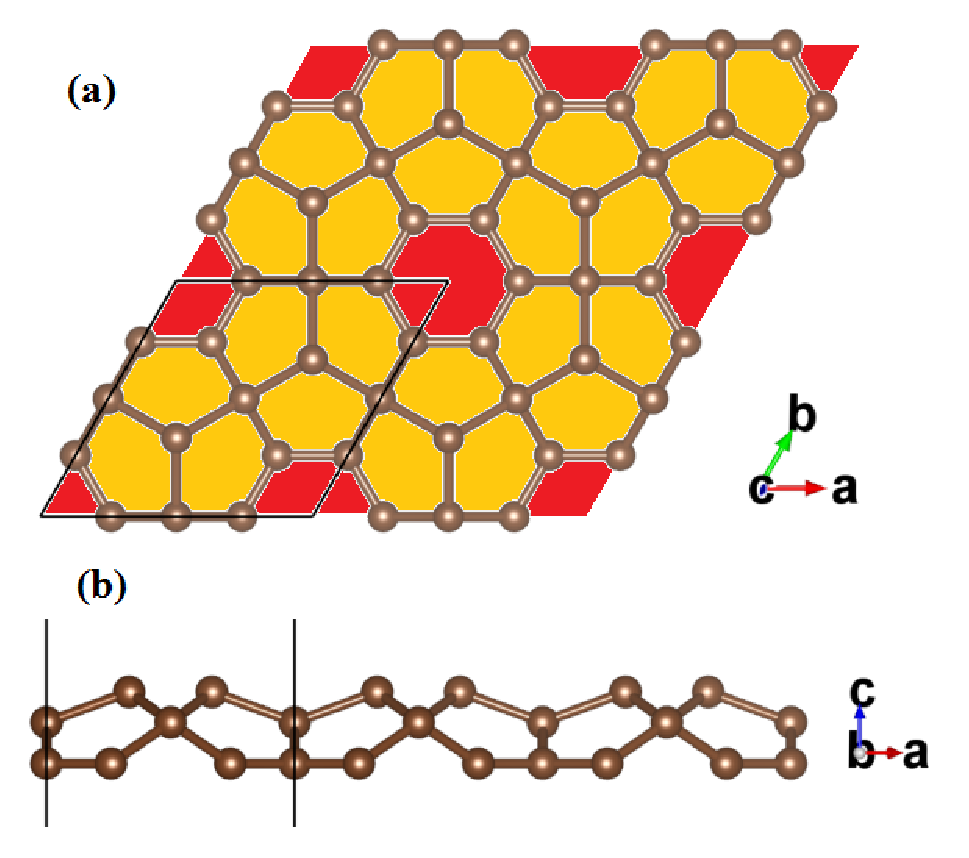
\includegraphics[width=0.6\linewidth]{PG_structure.eps}%   
\caption{Atomic structure of a 2$\times$2 supercell of monolayer ph-graphene. (a) Top view with hexagonal and pentagonal rings marked with red and yellow color, respectively; (b) Side view of the buckled structure. \label{structure} (Visualisation using VESTA \cite{vesta})}
\end{figure}

\subsection{Computational details}
\begin{footnotesize}
\begin{description}
\item[Simulation program:] VASP
\item[Energy cut-off:] 500 eV
\item[Pseudopotentials:] PBE-GGA(PAW)
\item[k points ($Gamma$ centered):] 15$\times$15$\times$1
\item[Vacuum:] 25~\AA
\item[Energy and force convergence criterion:] 10$^{-8}$ eV and 10$^{-7}$ eV/\AA, respectively
\item[Supercell for phonon calculation:] 3$\times$3$\times$1
\item[phonon calculation:] Density functional perturbation theory (DFPT)
\end{description}
\end{footnotesize}

\subsection{Bond hybridization and magnetic moment \label{res}}

The structure of the proposed 2D material is schematically shown in \autoref{structure}. It consists of hexagonal rings of C atoms surrounded by six pentagonal rings which share one edge with the hexagon and four with other pentagons. These hexagonal and pentagonal rings are arranged in a hexagonal lattice to form an infinite monolayer sheet. Considering the complex structure of this system, it is important to understand the hybridization of the electronic orbitals. For this, we calculate the hybridization index of the three C atoms that have a unique local environment, namely C1, C2 and C3 in \autoref{angle}, through Coulson's theorem: $1+\sqrt{n_1n_2}~cos\theta_{12}=0$, where $\theta_{12}$ is the interorbital angle between orbital 1 and 2 (see \autoref{angle}) and $n$ is the hybridization index.  $n$ corresponds to the index in the $sp^n$ notation and determines the relative fraction of $p$ orbitals with respect to the $s$ orbital. The sum of the $s$ fractions in all hybridized orbitals should equal 1, while it should be 3 for the sum of the $p$ fractions. 

\begin{figure}[htb]
\centering
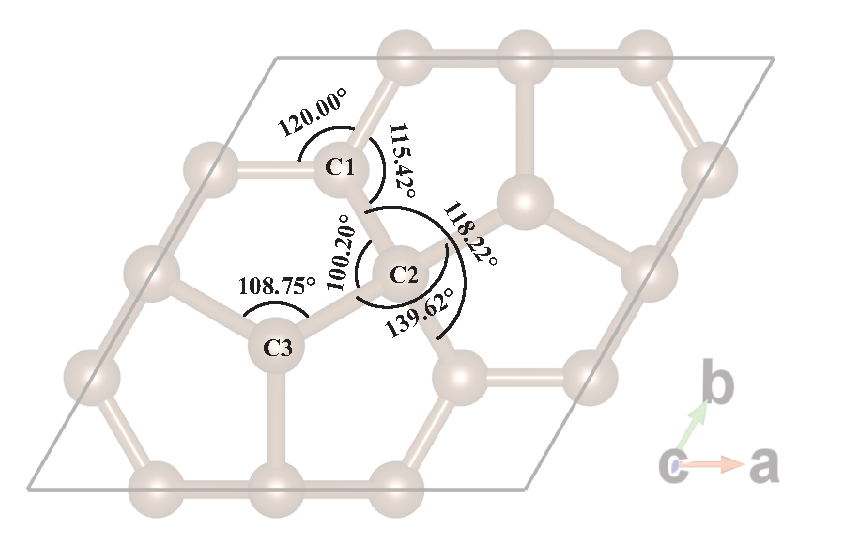
\includegraphics[width=0.7\linewidth]{PG_bond-angle.eps}%   
\caption{  Bond angles in the unit cell of monolayer ph-graphene. \label{angle}}
\end{figure}
  
\begin{table}[htb]
\centering
\caption{Orbital hybridization indices $n$ for four orbitals $\varphi$ of the C atoms in ph-graphene. \label{hybrid}}
\begin{tabular}{lcccc}
\hline\hline
Atom & $\varphi_1$ & $\varphi_2$ & $\varphi_3$ & $\varphi_4$  \\ \hline
C1 & 2.00 & 2.00 & 2.72 & 14.58 \\
C3 & 3.11 & 3.11 & 3.11 & 2.70 \\
\hline\hline
\end{tabular}
\end{table}

\begin{figure}[htb]
\centering
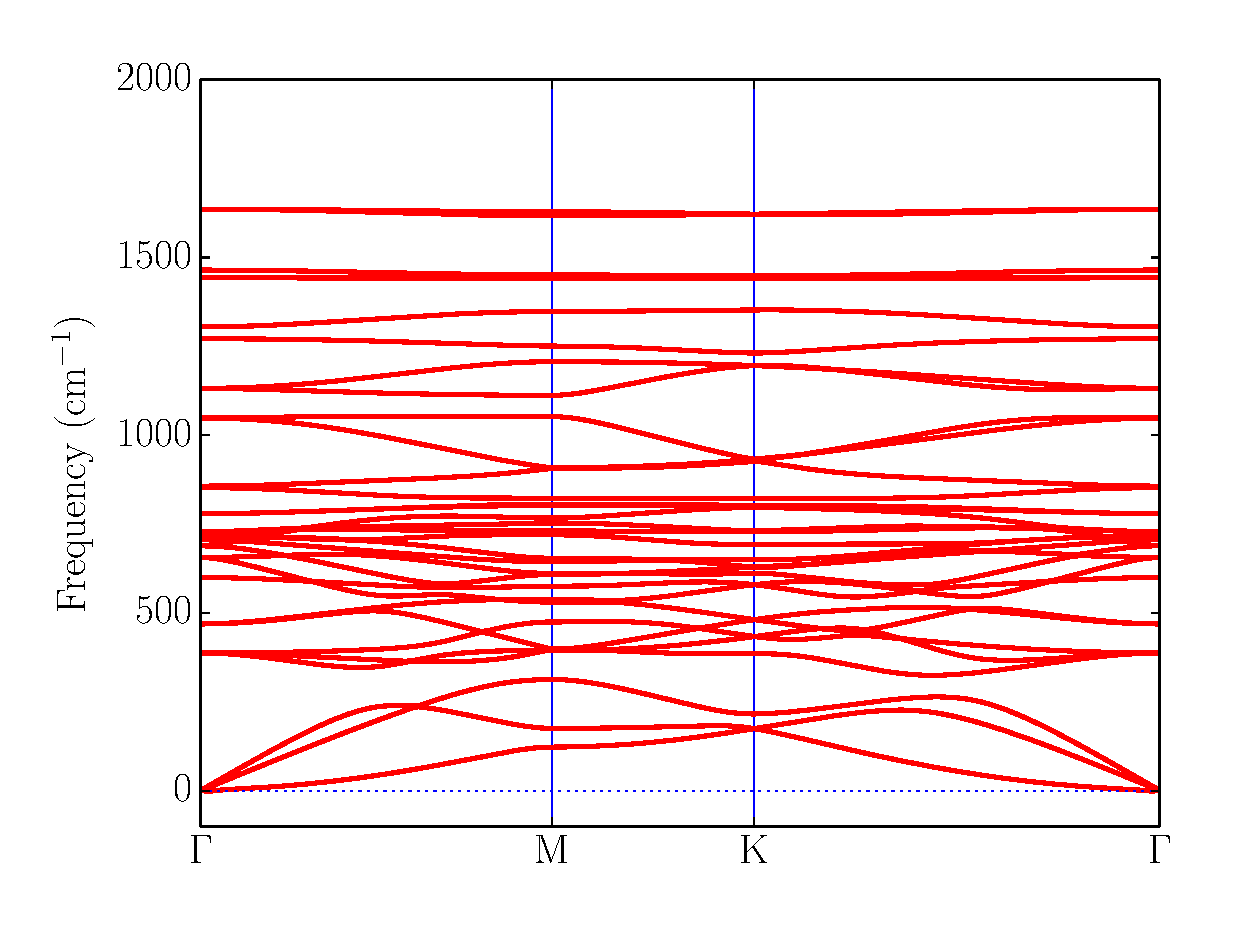
\includegraphics[width=0.7\linewidth]{PG_phonon.eps}%
\caption{  Phonon dispersion relation of monolayer ph-graphene. \label{phonon}}
\end{figure}

\begin{figure}[htbp]
\centering
  \begin{tabular}{c}
  \begin{subfigure}{0.7\textwidth}
    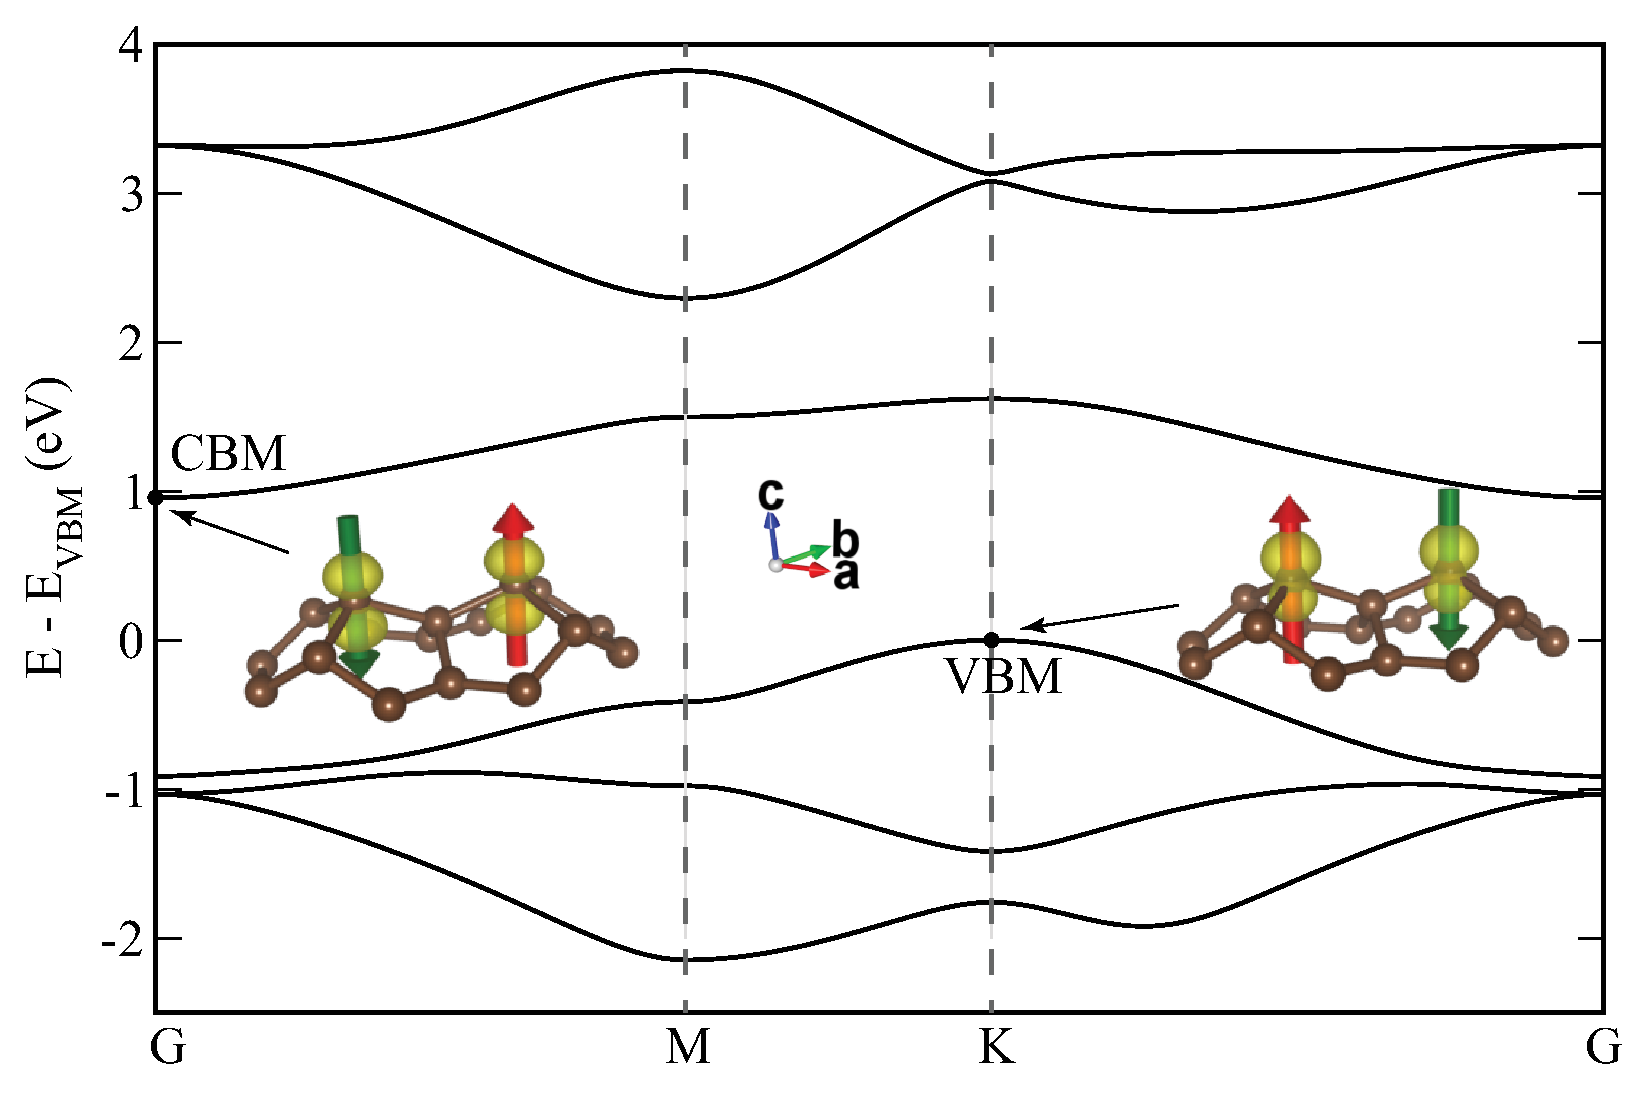
\includegraphics[width=\textwidth]{PG_band-AFM.eps}%   
    \caption{AFM}
  \end{subfigure} \\
  \begin{subfigure}{0.7\textwidth}
    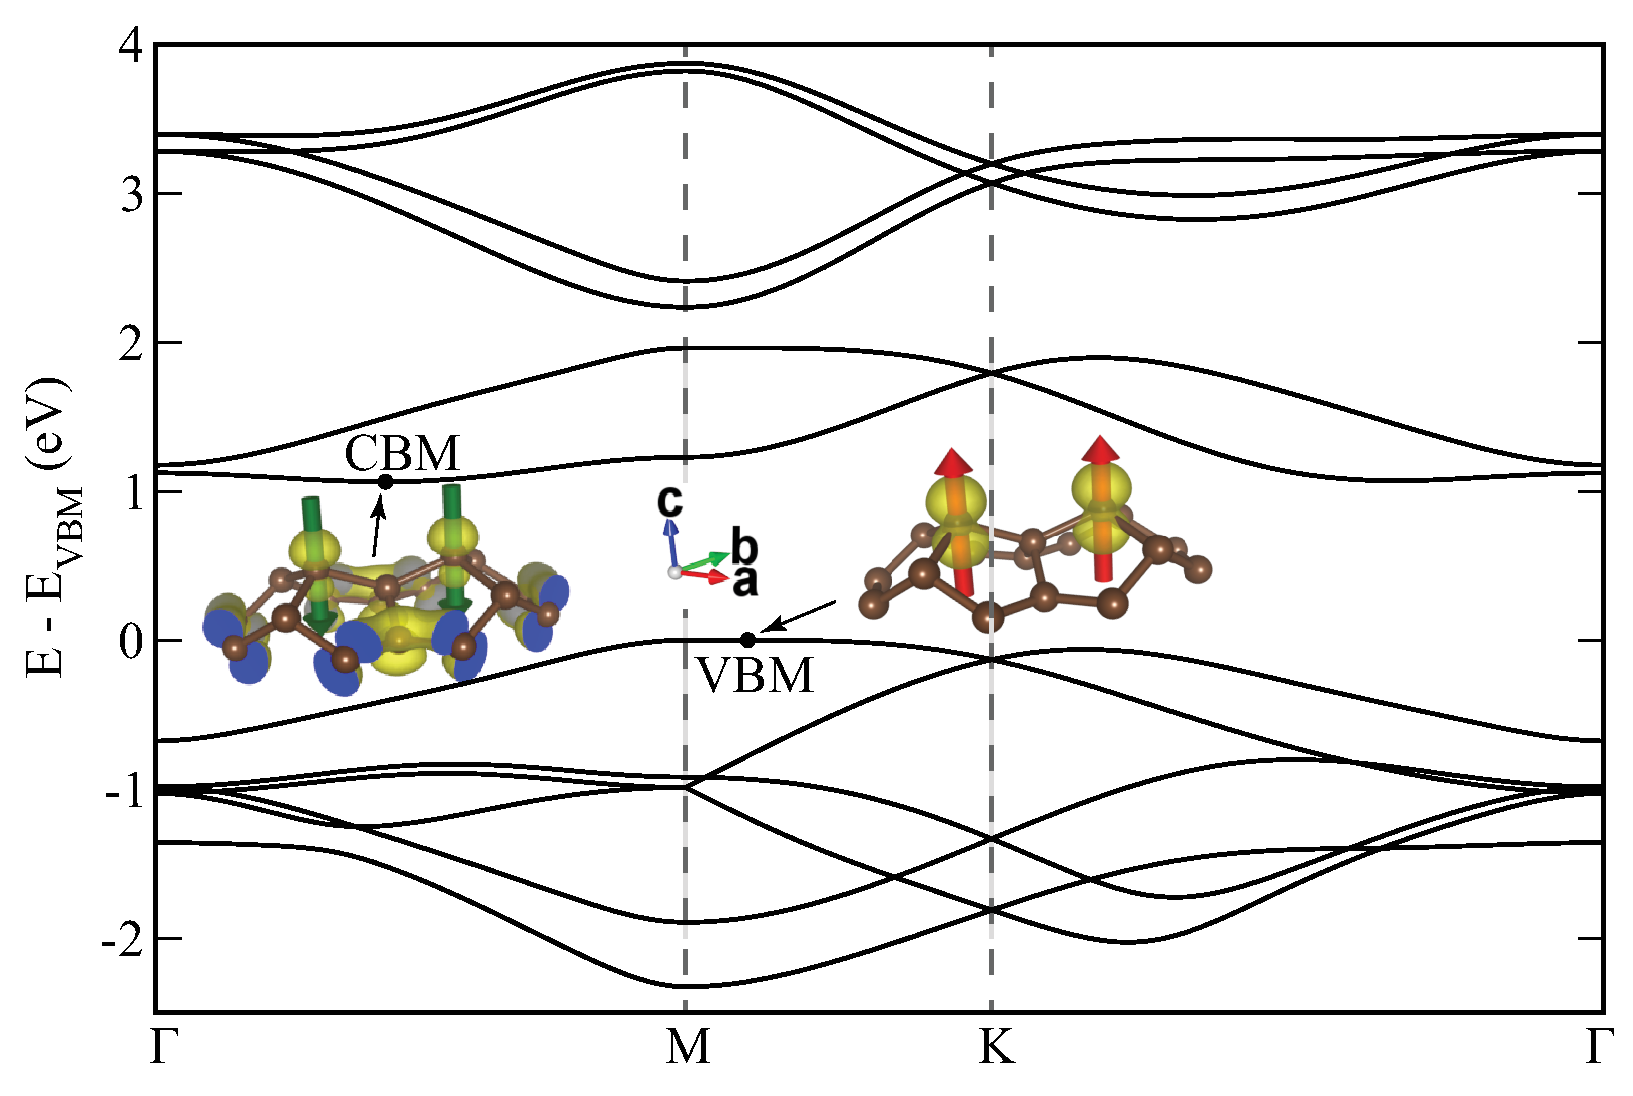
\includegraphics[width=\textwidth]{PG_band-FM.eps}%
    \caption{FM}
  \end{subfigure}    
  \end{tabular}
\caption{Electronic band structure of monolayer ph-graphene. The charge densities at the VBM and CBM in the unit cell are shown as insets. The arrows on the atoms indicate the orientation of their magnetic moments.\label{electronic} }
\end{figure}


In \autoref{hybrid}, we list the hybridization indices of the C1 and C3 orbitals, $\varphi$.  The C1 atom has two $sp^2$ orbitals with 120$^{\circ}$ interorbital angle and one $sp^{2.72}$. The latter gives rise to a partly buckled structure. The fourth C1 orbital has a large $p$ contribution, indicating that it is close to a $p_z$ orbital with little $s$ contribution, and induces $\pi$ bonding in the hexagonal rings. The C2 atoms have fourfold coordination and their hybridization should be close to $sp^3$. Due to geometric constraints, the bonds have strained angles\cite{coulson1949}. Finally, the C3 atom has four quasi-$sp^3$ orbitals of which three are used for nearest-neighbor $\sigma$ bonding. The electron in the fourth orbital remains unpaired and can give a local magnetic moment of 1 $\mu_B$ (Bohr magneton). There are two C3 atoms per unit cell which form a graphene-like subcrystal. The maximal magnetic moment per unit cell is therefore  2$\mu_B$ if the system is ferromagnetic. However, when we align these two magnetic moments antiparallel, the total energy is lowered by 12 meV per magnetic atom, which gives an AFM ground state. 

In comparison to penta-graphene, ph-graphene has a 76 mev/atom lower formation energy. However, it is about 0.9 eV/atom higher than that of graphene. The relatively high formation energy of ph-graphene as compared to graphene can be mainly attributed to the ``bent'' bonds of the C2 atoms due to geometric constraints. 

To check the dynamical stability of the ph-graphene structure we calculated its phonon spectrum (see \autoref{phonon}). Since there are no imaginary frequencies, we can conclude that the structure is dynamically stable.

The electronic band structure and the charge densities at the VBM and CBM are shown in \autoref{electronic}. Both the FM and AFM states exhibit indirect semiconducting character with a band gap (PBE) of 1.06 eV and 0.96 eV, respectively. The band edge states are mainly located on the magnetic atoms and the band gap separates states of opposite spin orientation. The hybridized $\varphi_4$ states (see above) on these atoms form a $\pi$ bonding network that resembles the $p_z$ $\pi$ bonding in graphene. For the FM state, the typical graphene-like band structure that results from this can be observed for the valence and conduction bands. These bands are separated due to the ferromagnetic exchange splitting in spin-up and spin-down states with a large gap in between. Note that the splitting between bonding and anti-bonding states at the $\Gamma$ point is strongly reduced with respect to graphene because of the larger interatomic distance separating the C3 atoms (3.1 {\AA} in ph-graphene \textit{vs} 1.4 {\AA} in graphene). Due to this increased bonding distance, the exchange interaction exceeds the bonding interaction and the system is magnetic in stark contrast to graphene where the $\pi$ bonding is much stronger.


\subsection{Summary}
In this work, we proposed a new type of stable monolayer carbon allotrope composed of pentagonal and hexagonal rings of carbon atoms. We explained the symmetry and the structure of the bonds that result in local magnetic moments. By comparing the total energy of the FM and AFM state, we conclude that the latter is the ground state. Our theoretical calculations give insight in the magnetic mechanism in this metal-free material, which can initiate further work on the exploration of magnetic properties of other 2D metal-free material. 


\section[Lithium battery related properties of MXenes/ \\ graphene heterostructure]{Lithium battery related properties of MXenes/ \protect\\ graphene heterostructure \footcite[This work is submitted:][]{Aierken2017.battery} \label{Li_MG}}

\subsection{Introduction}
Lithium ion batteries (LIBs) are widely used for electrochemical energy storage in electrical vehicles and portable electronic devices such as cell phones. The speed of development in these state of the art products mostly hinges on the progress in battery technology. The energy density and rate capability of both LIBs and sodium ion batteries (NIBs) are currently insufficient to satisfy costumers' needs. Therefore, the demand for metal based new generation batteries that have large reversible energy/power capacity, good cyclic stability and long life span is growing. Recently, rechargeable batteries based on 2D materials have received great attention because of their promising potential as anode materials with enhanced gravimetric and volumetric energy densities which is a key challenge in current rechargeable ion battery technology. For instance Mo$_2$C was shown to exhibit much better electrochemical properties in lithium-ion battery applications,\cite{mo2c-ref8}. Moreover, other 2D layered materials such as transition metal dichalcogenides,\cite{mo2c-ref11, mo2c-ref12}, black phosphorus\cite{mo2c-ref18, mo2c-ref20}, and MXenes (with M = Ti, V, Nb, Mo and X = C, N)\cite{mo2c-ref13} have also been widely investigated because of their high energy storage density and high rate capacity. However, experimental studies have shown that single type layered nanosheets inevitably restack during the cycling process, resulting in a rapid capacity fading and poor rate performance. 

Therefore, current interest has been directed towards heterostructured\cite{C5CS00937E,Pomerantseva_Gogotsi_2017} 2D materials. A clever design of vertical heterostructures from different 2D materials is expected to be beneficial for rapid electron transport and accelerated cation transport in the electrodes, and thus is expected to improve the rate performance in current battery technology\cite{Pomerantseva_Gogotsi_2017}. In addition, the negligible volumetric changes of in particular TMDs and MXenes under lithiation/de-lithiation processes, such that there is only 5\% in-plane lattice expansion in the Mo$_2$C lattice caused by Li intercalation\cite{C6TA01918H}, can minimize the intrinsic volumetric changes during charging/discharging processes which prolongs the cycling lifetime of the rechargeable batteries. Furthermore, combining different 2D materials is a promising way to adjust the interlayer distance to accommodate much larger (i.e. Na$^{+}$) and more polarized (i.e. Mg$^{2+}$) ions. For instance, lithium-ion capacity in excess of 750 mAh g$^{-1}$\cite{CELC:CELC201600059} has already been demonstrated for the batteries with MXene  electrodes, optimized with CNTs.

To this end, we  systematically investigated Li intercalation in vertical (van der Waals) heterostructures of MXenes and graphene for rechargeable battery applications. We only considered MXenes functionalized  with  OH and O, since the experimentally synthesized MXenes are often functionalized with various radicals due to chemical exfoliation. In addition, MXenes with low formula weights, such as Ti$_2$C, Nb$_2$C, V$_2$C and Sc$_2$C have been found to be most promising\cite{doi:10.1021/ja405735d} materials in battery applications due to their theoretically stated gravimetric capacity, which represents the amount of charge that can be stored per gram of material. Therefore, we considered only M$_2$CX$_2$ (where M=Sc, Ti, V and X=OH, O) monolayers in this study. V$_2$CX$_2$ is particularly important since it shows the largest Li$^+$ capacity of all MXenes tested under similar conditions\cite{doi:10.1021/ja508154e}. Another advantageous is that, compared to bilayer M$_2$CX$_2$, M$_2$CX$_2$/graphene hetorostructure has a much smaller weight, offering much larger storage capacity. 

We introduce the following nomenclatures in the following sections: M stands for the transition metal in MXenes; X stands for the functionalized group, i.e. OH or O; Gr stands for graphene; Li is intercalated Li atom (unless the concentration is stated it means only single Li atom intercalation); Monolayer and bilayer are denoted with mono- or bi- prefixes. For instance: bi-Ti$_2$CO$_2$+Li stands for bilayer Ti$_2$CO$_2$ with a single Li atom intercalation, and Ti$_2$CO$_2$+Gr+Li stands for heterostructure of Ti$_2$CO$_2$ on graphene with a single Li atom intercalation. 

\subsection{Computational details}
\begin{footnotesize}
\begin{description}
\item[Simulation program:] VASP
\item[Energy cut-off:] 500 eV
\item[Pseudopotentials:] PBE-GGA(PAW)
\item[k points ($\Gamma$ centered):] 7$\times$7$\times$1 to 11$\times$11$\times$1
\item[Vacuum:] 30~\AA
\item[Energy and force convergence criterion:] 10$^{-5}$ eV and 10$^{-3}$ eV/\AA, respectively
\item[vdW interactions:] DFT-D3 method \citet{Grimme2011} including Becke-Johnson damping
\item[Charge analysis:] Bader analysis \cite{Bader1,Bader2,Bader3,Bader4}
\end{description}
\end{footnotesize}
\vspace{0.5cm}

In addition, we calculated diffusion barriers for Li ions using the climbing-image nudge elastic (cNEB) method as implemented in the VASP transition state tools\cite{c-neb1,c-neb2}. The cNEB method is an efficient method to determine the minimum energy diffusion path between two given positions. We used at least 7 images, including initial and final positions, for cNEB calculations. The atomic positions and energy of the images were then relaxed until the largest norm of the force orthogonal to the path is smaller than 0.01 eV/{\AA}. 

\subsection{Heterostructure stacking types}

\begin{figure}[htb]
\centering
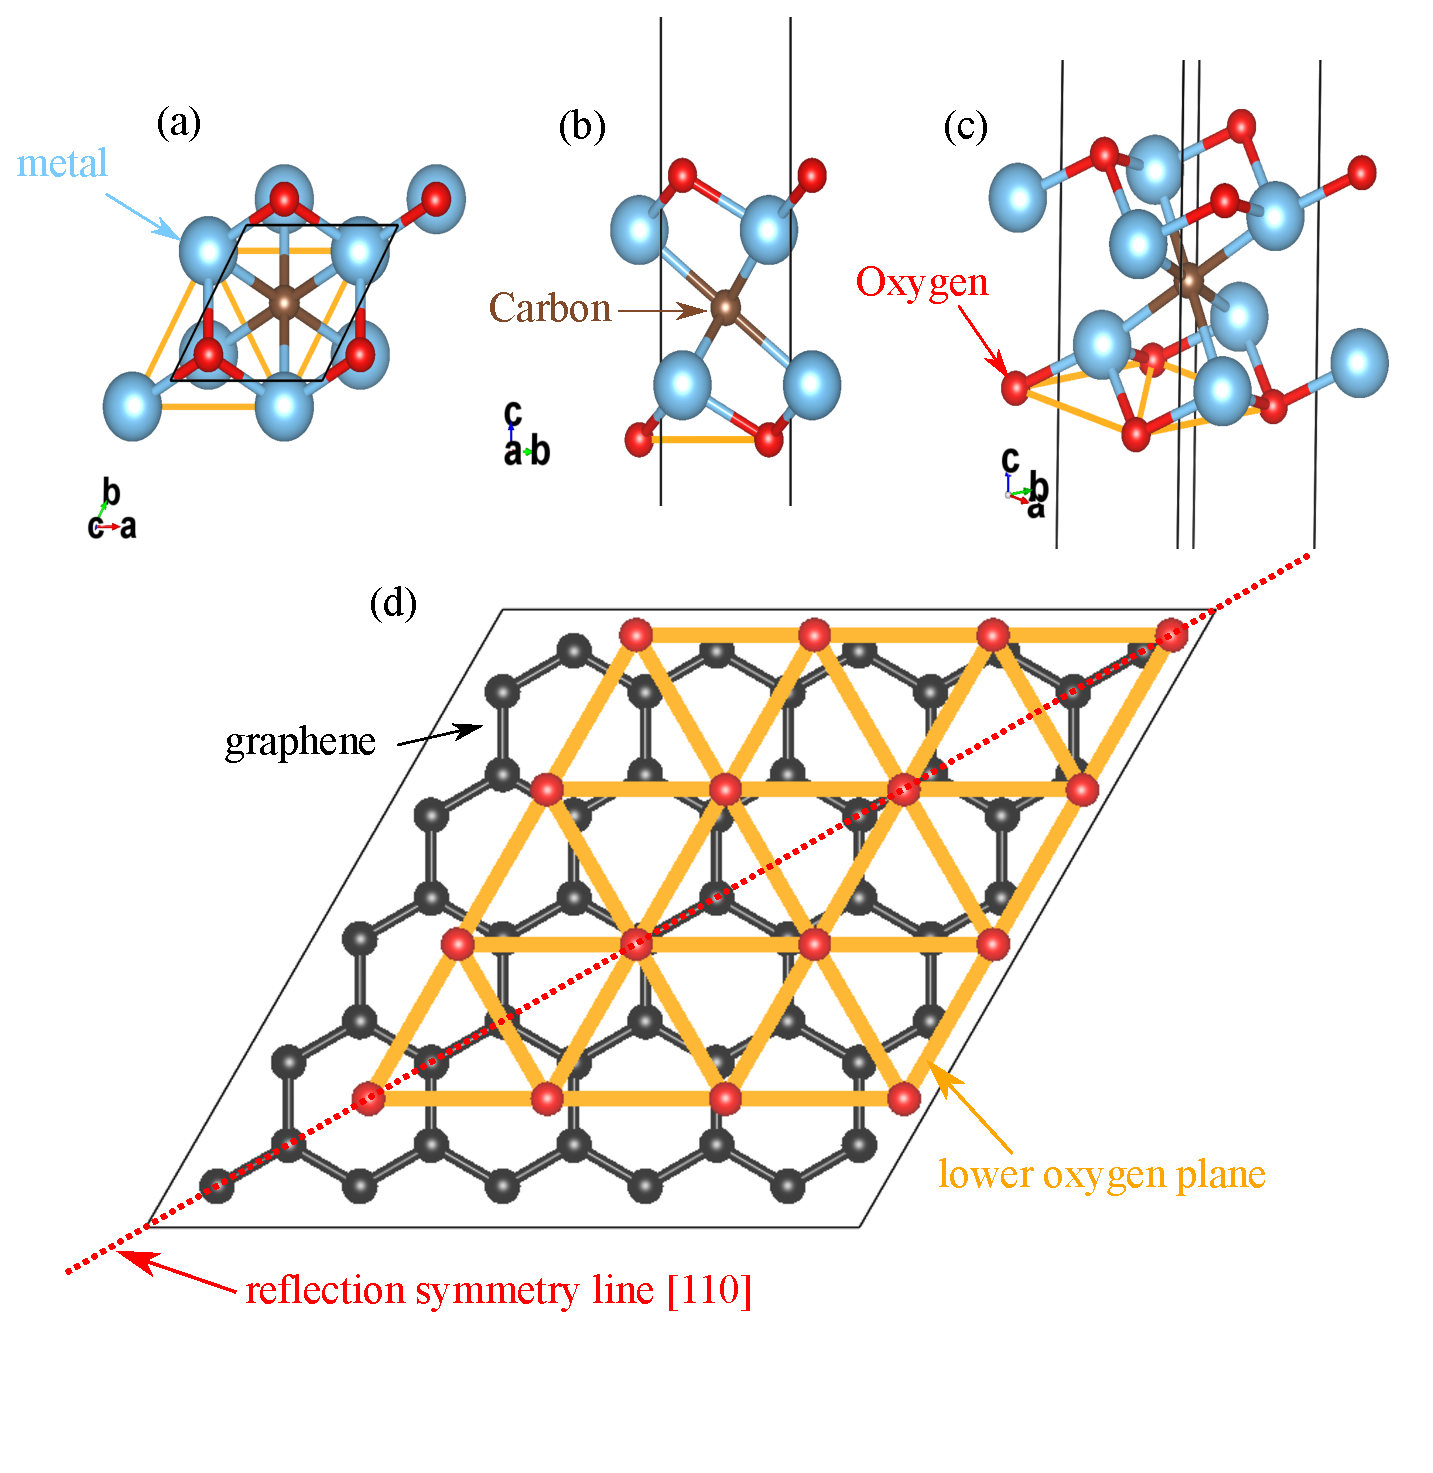
\includegraphics[width=0.8\linewidth]{stacking.eps}%
\caption{An example structure of mono-Ti$_2$CO$_2$ with (a) top view, (b) side view, and (c) tilted view. (d)  Simplified example of the M$_2$CX$_2$+Gr heterostructure in its ground state stacking.  \label{Li_stacking}}
\end{figure}

\begin{table}[htb]
\centering
\caption{A comparison of different MXenes systems: monolayer, bilayer, and heterostructure. $d$ is the interlayer distance and is defined as shown in \autoref{inter-dist}. $E_b$ is the binding energy of the system with respect to its components, e.g bilayer with respect to monolayers. Only the ground state stacking of M$_2$CX$_2$+Gr is reported.} 
\label{tableI}
\begin{tabularx}{0.8\linewidth}{XXXX}
\hline
Material      & Structure                         & $d$               & $E_b$               \\
              &                                    & \AA                & eV/atom \\ \hline
\multirow{2}{*}{graphene}      & bi-Gr (AB)                                               & 3.277                    & -0.024                        \\
              & bi-Gr (AA)                                                & 3.325                    & -0.020                         \\ \multicolumn{4}{c}{}\\
\multirow{2}{*}{Sc$_2$CO$_2$}    & bi-Sc$_2$CO$_2$                                                   & 2.294                 & -0.029                         \\
              & Sc$_2$CO$_2$+Gr                                                   & 3.067                   & -0.022                         \\
\multicolumn{4}{c}{}\\              
\multirow{2}{*}{Sc$_2$C(OH)$_2$} & bi-Sc$_2$C(OH)$_2$                                                   & 0.598                  & -0.025                         \\
              & Sc$_2$C(OH)$_2$+Gr                                                     & 2.191                  & -0.027                         \\
\multicolumn{4}{c}{}\\              
\multirow{2}{*}{Ti$_2$CO$_2$}    & bi-Ti$_2$CO$_2$                                                & 2.396                   & -0.027                         \\
              & Ti$_2$CO$_2$+Gr                                                   & 3.000                    & -0.018                         \\
\multicolumn{4}{c}{}\\              
\multirow{2}{*}{Ti$_2$C(OH)$_2$} & bi-Ti$_2$C(OH)$_2$                                               & 0.399                   & -0.024                         \\
              & Ti$_2$C(OH)$_2$+Gr                                                  & 2.097                    & -0.034                         \\
\multicolumn{4}{c}{}\\             
\multirow{2}{*}{V$_2$CO$_2$}     & bi-V$_2$CO$_2$                                                 & 2.394                    & -0.025                         \\
              & V$_2$CO$_2$+Gr                                                     & 2.867                    & -0.022                         \\
\multicolumn{4}{c}{}\\              
\multirow{2}{*}{V$_2$C(OH)$_2$}  & bi-V$_2$C(OH)$_2$                                              & 0.398                    & -0.011                         \\
              & V$_2$C(OH)$_2$+Gr                                                 & 2.779                    & -0.035                         \\ \hline                     
\end{tabularx}
\end{table}

First of all, we constructed the MXene-Graphene heterostructures by considering super cells such that we have a minimum lattice mismatch between the layers. Therefore, heterostructures with a 3$\times$3 super cell of Sc$_2$CO$_2$ or Sc$_2$C(OH)$_2$ with a 4$\times$4 super cell of graphene, a  4$\times$4 super cell of Ti$_2$CO$_2$ or Ti$_2$C(OH)$_2$ with a 5$\times$5 super cell of graphene, and a 5$\times$5 super cell of V$_2$CO$_2$ or V$_2$C(OH)$_2$ with a 6$\times$6 super cell of graphene were constructed, see \autoref{Li_stacking} for a representative example. In order to find out the ground state stacking type of these, M$_2$CX$_2$+Gr heterostructures, we calculated the binding energy of possible stacking configurations by shifting the M$_2$CX$_2$ layer over the unit cell of graphene on a uniform mesh. In the course of these simulations, each layer in the heterostructure is regarded rigid where only the interlayer distance is allowed to relax. The corresponding binding energy per atom, $E_b$ was calculated as follows:
\begin{equation}
E_b=\frac{1}{N}[E(\mathrm{M}_2\mathrm{C}\mathrm{X}_2+\mathrm{Gr})-E(\mathrm{M}_2\mathrm{C}\mathrm{X}_2)-E(\mathrm{Gr})],
\end{equation}
where $E$(M$_2$CX$_2$+Gr), $E$(M$_2$CX$_2$) and $E$(Gr) are the total energies of M$_2$CX$_2$+Gr, mono-M$_2$CX$_2$ and Gr, respectively. $N$ is the total number of atoms in the super cell. In \autoref{tableI}, the calculated $E_b$ and the interlayer distance for M$_2$CX$_2$+Gr are given  for all the considered systems. The results for graphene bilayer are also given as reference. The interlayer binding energy and the distance of AB stacked bilayer graphene are 24 meV/atom and 3.28 {\AA}, respectively. Our calculations agree very well with a recent work in which quantum Monte Carlo simulations predicted a 18 meV/atom binding energy and 3.38 {\AA} interlayer separation for bilayer graphene\cite{PhysRevLett.115.115501}. The calculated binding energies (i.e. $E_b$) are negative for all the considered heterostructures, demonstrating the stability of each system against phase separation. The magnitude of $E_b$ for the ground state stacking in MXene oxides/graphene are comparable to that of bilayer graphene, whereas the hydroxides/graphene are slightly stronger bonded due to the extra hydrogen bonds. The differences in binding energy among different MXenes that have the same functionalized group are negligible.



\begin{figure}[htb]
\centering
\includegraphics[width=0.8\linewidth]{inter_dist.eps}%
\caption{The optimized locations of single Li atoms in different structures and the definition of interlayer distance $d$, which ignores the Li atom layer.\label{inter-dist}.}
\end{figure}

\subsection{Single Li intercalation and its binding energy}

\begin{figure}[htb]
\centering
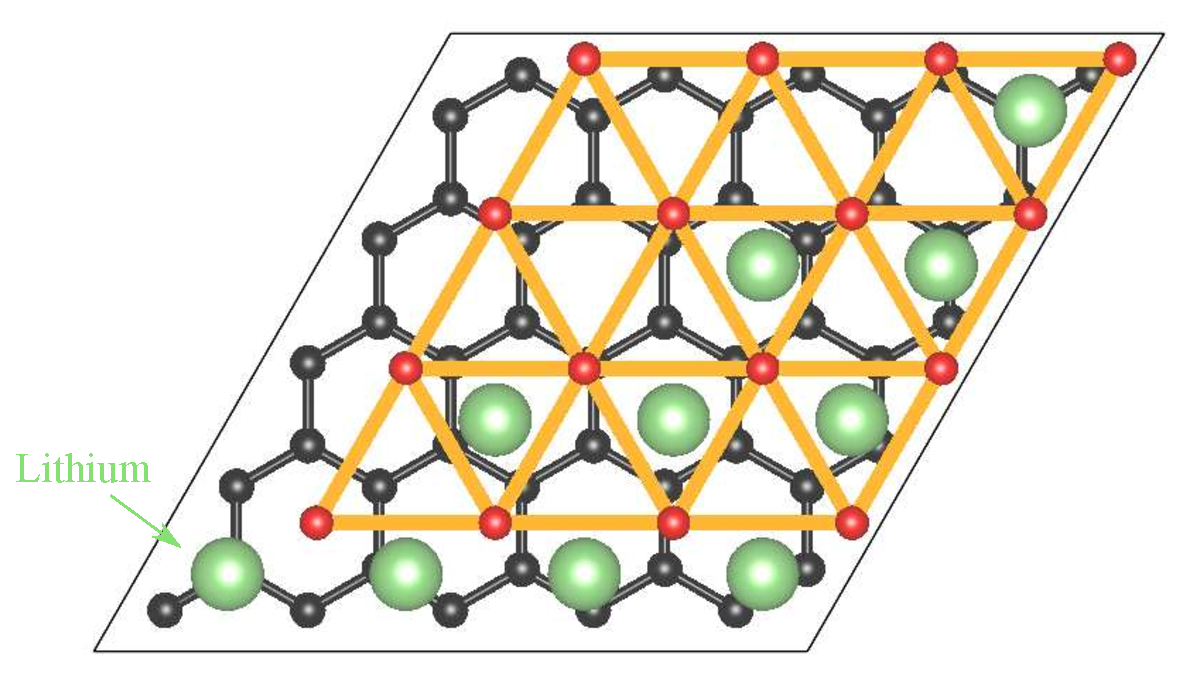
\includegraphics[width=0.8\linewidth]{sites.eps}%
\caption{The locations of Li atoms intercalation between Ti$_2$CO$_2$+Gr heterostructure as an example.  \label{sites}}
\end{figure}

Using the calculated ground state stacking types of all the M$_2$CX$_2$+Gr heterostructures, we investigated the Li intercalation in these structures. To systematically uncover the potential of M$_2$CX$_2$+Gr heterostructures for battery applications, we also considered Li intercalation on mono-M$_2$CX$_2$, within bi-M$_2$CX$_2$ and within bi-Gr. These additional reference calculations were performed with the same system dimensions, or equivalently the same Li atom concentration, as in the corresponding heterostructures.

Previous studies\cite{Guo2015,Samad2016,Lee2012} pointed out that the strongest binding of the Li atoms occurs for bilayer heterostructure. They reported a non-binding character of Li atoms on the surface of few-layer graphene. Therefore, in this study, we limited ourselves to the intercalation between M$_2$CX$_2$ and graphene. In addition, inspired by the previous study\cite{doi:10.1063/1.4939745} on the location of the Li absorption site in M$_2$CX$_2$ multilayer system, we found that the intercalated Li atom is bound close to the M$_2$CX$_2$ layer and far from graphene, and it resides between three O atoms. Thus, each formula unit of M$_2$CX$_2$ in heterostructure can accommodate one Li atom.  Additional Li atoms occupy the same position in other unit cells, as shown in \autoref{sites}. Note that the ground state stacking has reflection symmetry, and therefore we may limit ourselves to investigate Li positions only on one side of the symmetry line [110] for  single Li absorption.  A strong binding between Li and M$_2$CX$_2$+Gr bilayer is necessary to avoid the formation of metallic lithium, which well improves the safety and reversibility of lithium-ion batteries. Therefore, we need to make sure that the reported Li binding energy as large as possible. We calculated all the possible adsorption sites between the two layers, here I only present the ground state configuration.

The binding energy, $E_{b}^{Li}$, for Li intercalated systems is defined through the following equation:
\begin{equation}
E_{b}^{Li}=\frac{1}{x}[E(\mathrm{with~}x\mathrm{Li})-E(\mathrm{without~Li})-xE(\mathrm{Li})],
\end{equation}
	where $E(\mathrm{with~}x\mathrm{Li})$ and $E(\mathrm{without~Li})$ are the total energies of system with and without $x$ Li atoms, respectively. $E(\mathrm{Li})$ is the total energy of a Li atom in its most stable bcc bulk structure. Here, a more negative binding energy indicates a more favourable exothermic binding of Li.

In \autoref{my-label}, the results for three different promising systems are shown. For comparison, we also calculated Li intercalation in AA and AB stacked graphene bilayers. While the latter is more stable than the former for the pristine systems, the former is energetically more favorable for Li intercalation, which is consistent with previous calculations\cite{PhysRevB.93.245438}, see \autoref{my-label}.  The LiC$_{64}$ (4$\times$4 bilayer graphene) in AA configuration is energetically favorable to accommodate single Li between bilayer, while the Li atom will not bind at all in the AB stack bilayer configuration. However, the magnitude of the binding energy generally is small as compared to the heterostructure due to the strong interaction of Li with the M$_2$CO$_2$ layer.


Our results can be summarized as follows: 		
(1) All the systems related to Sc$_2$CO$_2$ experience severe structural distortion upon Li interactions. Two or three of the C atoms in the Sc$_2$CO$_2$ move towards each other and show the tendency to cluster. Therefore, this type of system is unstable for Li intercalation.  
(2) The binding of a Li atom on mono-M$_2$C(OH)$_2$ is not favorable. This can be attributed to the Coulomb repulsion between positively charged Li ion and H atoms. 
(3) When going from mono- to bi-M$_2$C(OH)$_2$+Li, Li adsorption is made stable again through the van der Waals interaction that competes with foregoing repulsive interaction. 
(4) Mono-M$_2$CO$_2$+Li,  bi-M$_2$CX$_2$+Li and M$_2$CX$_2$+Gr+Li exhibit the strongest adsorption for Li atoms. The calculated $E_{b}^{Li}$ value at the largest binding energy site is -1.87 eV/atom for the mono-Ti$_2$CO$_2$ and -2.97 eV/atom for the mono-V$_2$CO$_2$. In the case of M$_2$CX$_2$+Gr+Li, we observed that $E_{b}^{Li}$ slightly decreases for M=Ti and V and X=O.  This may be correlated to the reduced vdW interaction with respect to the pristine bilayers due to the increase in interlayer separation.   
(5) We have identified three promising candidates with large Li atom adsorption energy, namely Sc$_2$C(OH)$_2$+Gr+Li, Ti$_2$CO$_2$+Gr+Li and V$_2$CO$_2$+Gr+Li. Therefore, for the rest of the paper, we will focus on these three systems and will study the kinetics of Li diffusion. 

\begin{table*}[htbp]
{\footnotesize
\centering
\caption{A comparison of different MXenes systems: monolayer, bilayer, and heterostructure with Li intercalation. $d$ is the interlayer distance and is defined as shown in \autoref{inter-dist}. $E_b^{Li}$ is the binding energy of a single Li atom. Only the largest binding energy of Li atom is reported, i.e. ground state adsorption site. $L_{min}$ is the shortest bond length of a Li atom with others. The charge transfer from a Li atom to a heterostructure is in units of $e$. For consistency of the Li concentrations, all monolayer and bilayer systems use the same dimensions as in the corresponding heterostructures. Three different sizes of bi-Gr are presented to compare with the heterostructures with corresponding size of Gr.}  
\label{my-label}
\begin{tabularx}{\textwidth}{llcccc}
\hline
Material      & Structure                         & $d$                & $E_b^{Li}$               & $L_{min}$ & Li charge transfer   \\
              &                                   & \AA                       & eV/atom                             & \AA                       & e                \\ \hline
\multirow{4}{*}{graphene}      & 4$\times$4 bi-Gr (AB)+Li                 & 3.591                    & 0.030                          & 2.060                     & 0.873                        \\
              & 4$\times$4 bi-Gr (AA)+Li                 & 3.616                                                                            & -0.232                         & 2.344                     & 0.868                        \\
              & 5$\times$5 bi-Gr (AA)+Li                  & 3.617                                                                          & -0.283                         & 2.344                     & 0.878                        \\
              & 6$\times$6 bi-Gr (AA)+Li                  & 3.636                                                                         & -0.336                         & 2.352                     & 0.879                        \\ 
& & & & \\              
\multirow{3}{*}{Sc$_2$CO$_2$ (unstable)}    & mono-Sc$_2$CO$_2$+Li  & -  & -9.986  & 2.024  & 0.898 \\
              & bi-Sc$_2$CO$_2$+Li   & 1.791              & -32.646 & 2.208  & 0.902 \\
              & Sc$_2$CO$_2$+Gr+Li     & 2.874              & -19.885 & 1.958  & 0.887 \\ 
              & & & & \\
\multirow{3}{*}{Sc$_2$C(OH)$_2$} &mono-Sc$_2$C(OH)$_2$+Li                                            & -                        & 0.048                          & 1.918                     & 0.869                        \\
              &bi-Sc$_2$C(OH)$_2$+Li                                              & 0.548                     & -0.309                         & 2.050                     & 0.885                        \\
              &Sc$_2$C(OH)$_2$+Gr+Li                                                   & 2.278                   & -0.941                         & 1.953                     & 0.877                        \\ 
              & & & & \\
\multirow{3}{*}{Ti$_2$CO$_2$}    &mono-Ti$_2$CO$_2$+Li                                            & -                         & -1.870                         & 1.994                     & 0.912                        \\
              &bi-Ti$_2$CO$_2$+Li                                                 & 2.480                   & -2.308                         & 2.047                     & 0.886                        \\
              &Ti$_2$CO$_2$+Gr+Li                                                   & 2.976                   & -1.729                         & 1.993                     & 0.887                        \\ 
              & & & & \\
\multirow{3}{*}{Ti$_2$C(OH)$_2$} &mono-Ti$_2$C(OH)$_2$+Li                                              & -                                     & 0.146                          & 1.926                     & 0.792                        \\
              &bi-Ti$_2$C(OH)$_2$+Li                                              & 0.599                   & -0.431                         & 2.004                     & 0.879                        \\
              &Ti$_2$C(OH)$_2$+Gr+Li                                                  & 2.090                   & -0.229                         & 1.941                     & 0.875                        \\ 
              & & & & \\
\multirow{3}{*}{V$_2$CO$_2$}     &mono-V$_2$CO$_2$+Li                                              & -                        & -2.791                         & 1.975                     & 0.921                        \\
              &bi-V$_2$CO$_2$+Li                                                 & 2.500               & -3.573                         & 2.009                     & 0.887                        \\
              &V$_2$CO$_2$+Gr+Li                                                  & 2.779                  & -2.537                         & 1.957                     & 0.891                        \\ 
              & & & & \\
\multirow{3}{*}{V$_2$C(OH)$_2$}  &mono-V$_2$C(OH)$_2$+Li                                            & -                        & -0.175                         & 1.878                     & 0.860                       \\
              &bi-V$_2$C(OH)$_2$+Li                                                 & 0.395                   & -1.336                         & 1.995                     & 0.878                        \\
              &V$_2$C(OH)$_2$+Gr+Li                                                 & 2.080                  & -0.304                         & 1.912                     & 0.878  \\ \hline                     
\end{tabularx}
}
\end{table*}


\subsection{Effect of Li concentration}

\begin{figure}[htbp]
\centering
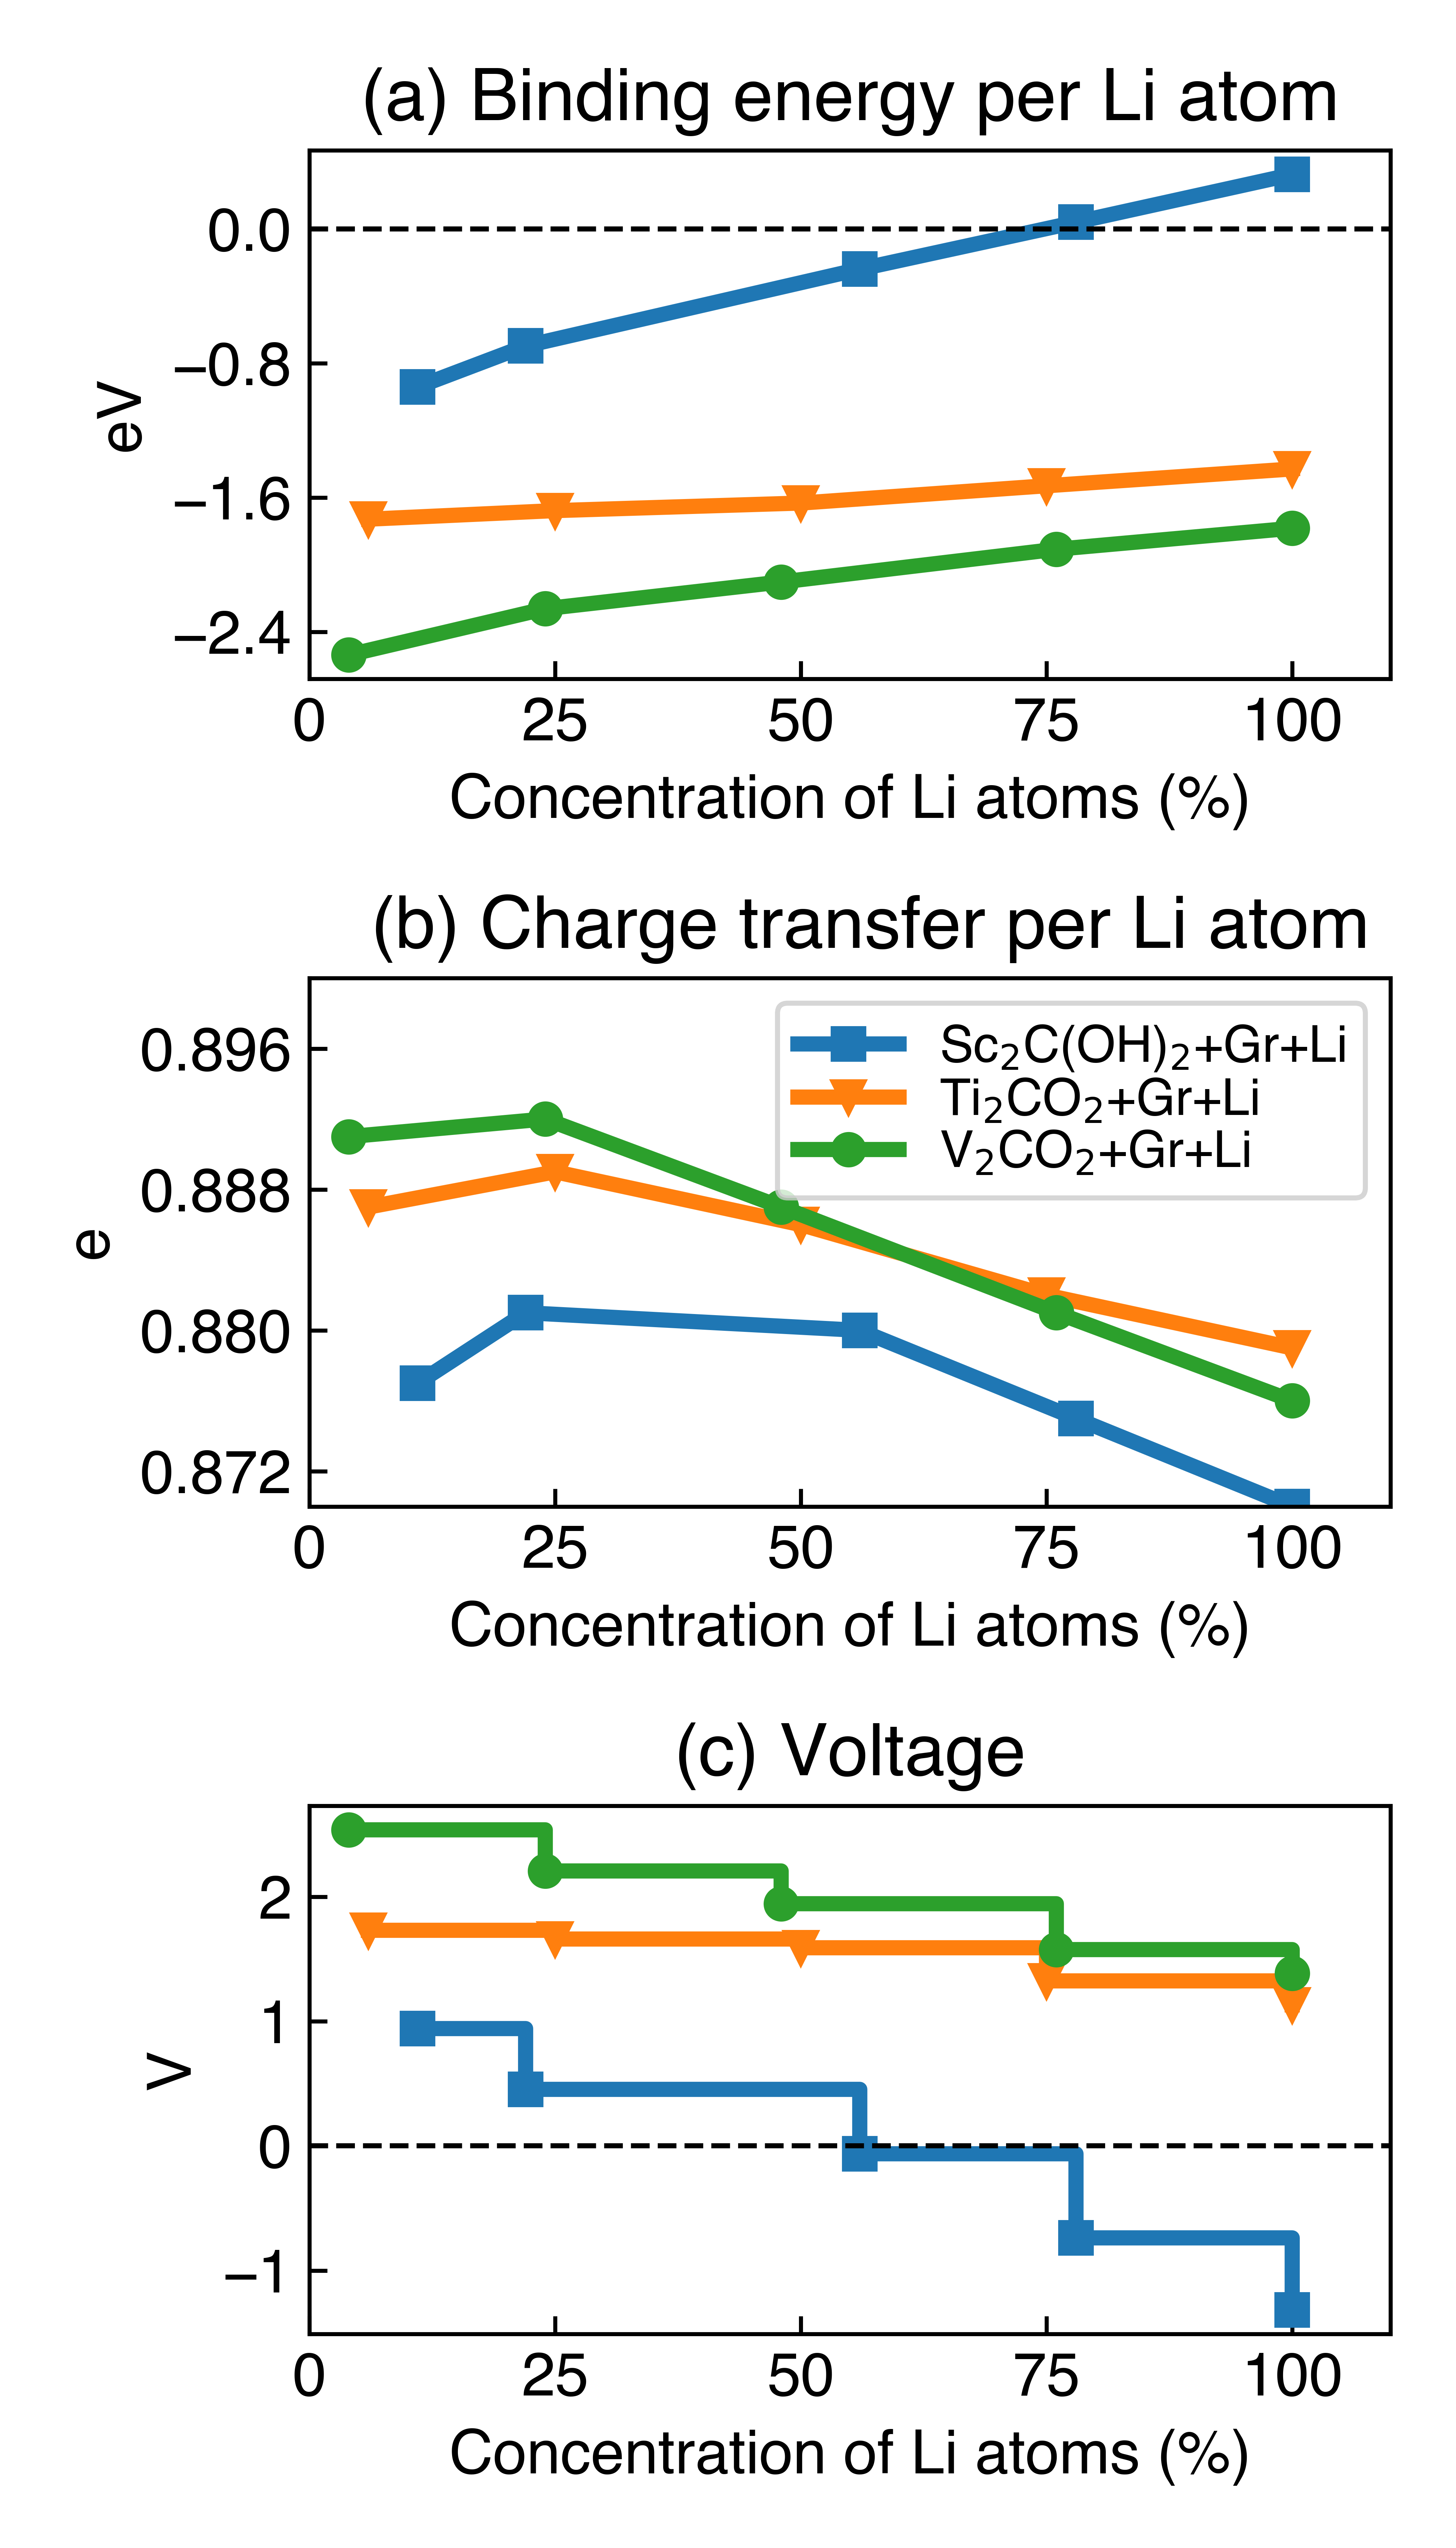
\includegraphics[width=0.6\linewidth]{Li_con.png}%
\caption{The average binding energy (a), the average charge transfer (b) of Li atoms, and the voltage profile of M$_2$CX$_2$+Gr heterostructure as a function of Li concentration. \label{concenration}}
\end{figure}

As a next step, we investigated the effect of Li ion concentration on the physical properties of M$_2$CX$_2$+Gr+Li heterostructures. Here, the concentration is defined as the ratio of the number of Li atoms and the number of formula unit of M$_2$CX$_2$ in the heterostructures (e.g. 100\% corresponds to one Li atom for each formula unit). \autoref{concenration}(a) shows the variation of the average $E_{b}^{Li}$ as a function of concentration of Li ions (i.e. $x$). As the number of intercalated Li increases,  the average $E_{b}^{Li}$ decreases gradually. The reduction in binding energy is due to two main factors; One is the weak electrostatic attraction between M$_2$CX$_2$+Gr host and the Li cations, and the other one is the enhanced Li-Li repulsion at high Li concentration. The former is correlated with the reduction of charge transfer from the Li atom to M$_2$CX$_2$+Gr complex at high concentrations, as shown in \autoref{concenration}(b). Similarly, the latter is due to the reduction of interatomic distances between positively charged Li ions. Above a critical concentration value, namely 80\%,  $E_{b}^{Li}$ becomes positive for Sc$_2$C(OH)$_2$+Gr+Li, and the system becomes energetically unstable for further Li insertion. $E_{b}^{Li}$ is always negative for Ti$_2$CO$_2$+Gr+Li and V$_2$CO$_2$+Gr+Li, suggesting that these heterostructures are stable against Li intercalation, and thus we can safely disregard the phase separation into individual monolayers and bulk Li at high concentrations. In other words, the Ti$_2$CO$_2$+Gr+Li and V$_2$CO$_2$+Gr+Li structures are highly stable even for high Li concentrations. For V$_2$CO$_2$+Gr+Li (Ti$_2$CO$_2$+Gr+Li), $E_{b}^{Li}$ may vary by about 1 (0.5) eV as a function of Li concentration. Recently, \citet{doi:10.1021/acsami.5b03863}reported that V$_2$CO$_2$ undergoes a reversible structural transformation during the adsorption of Li. We also checked the possibility of such structural transformation for V$_2$CO$_2$+Gr bilayer and we found that the presence of graphene prevents the transformation of V$_2$CO$_2$. Our results clearly demonstrated that Ti$_2$CO$_2$+Gr+Li and V$_2$CO$_2$+Gr+Li can be utilized as an anode material for high capacity Li ion batteries.


Another important point is how the structural stability of Ti$_2$CO$_2$+Gr+Li and V$_2$CO$_2$+Gr+Li is affected as the Li ion concentration is increased. We found that an increase in the number of Li ions leads to a small expansion in the in-plane lattice constants.  For instance, the in-plane lattice constant of both V$_2$CO$_2$+Gr+Li and Ti$_2$CO$_2$+Gr+Li increase by less than 1\%.   Besides, we did not observe any  severe  lengthening of the surface Ti/V-O bonds and
shortening of Li-O bonds for both Ti$_2$CO$_2$+Gr+Li and V$_2$CO$_2$+Gr+Li heterostructures. For instance,
Li-O bond length decreases with most 3\% with increasing Li concentration.   
It is also found that Li intercalation slightly enlarges and later reduces the interlayer separation as the Li concentration increases. The calculated interlayer separation suggests that we can have at most 0.5 {\AA} expansion as a result of Li intercalation. These results clearly show that these layered M$_2$CX$_2$+Gr heterostructures possess a reversible reaction process, which is necessary for rechargeable ion batteries and thus they can effectively defy the volume expansion problem faced by present day electrode materials. However, Sc$_2$C(OH)$_2$+Gr is unstable against Li loading at higher concentration. 



\subsection{Electrochemical properties}

In order to gain insight into the electrochemical properties of the Li intercalation process into the M$_2$CX$_2$+Gr heterostructure, the open-circuit-voltage was obtained by calculating the averaged half cell voltage over a range of metal ion concentrations $x$, where $x_1\leq x\leq x_2$, using,
\begin{equation}
V\approx\frac{E_{\mathrm{M}_2\mathrm{C}\mathrm{X}_2+\mathrm{Gr}+\mathrm{x_1Li}}-E_{\mathrm{M}_2\mathrm{C}\mathrm{X}_2+\mathrm{Gr}+\mathrm{x_2Li}}+(x_2-x_1)E_{\mathrm{Li}}}{(x_2-x_1)e}
\end{equation}
where $E_{\mathrm{M}_2\mathrm{C}\mathrm{X}_2+\mathrm{Gr}+\mathrm{Li}_{x_1}}$ and $E_{\mathrm{M}_2\mathrm{C}\mathrm{X}_2+\mathrm{Gr}+\mathrm{Li}_{x_2}}$ are the total energies of the M$_2$CX$_2$+Gr heterostructure with $x_1$ and $x_2$ Li intercalated, respectively.  $E_{\mathrm{Li}}$ is the total energy of bulk bcc Li.  First of all, our calculations show that the charging voltage for Li intercalation decreases with increasing in Li ion concentration, as clearly seen in \autoref{concenration}(c). The calculated average voltage corresponding to Sc$_2$C(OH)$_2$+Gr+Li is negative for a Li ion concentration $x$ larger than 55\%. As mentioned above, a phase transition should be expected for the concentrations larger than this critical value. Our results are consistent with a recent work reporting that H and/or OH should be avoided if possible since they result in a lower capacity and negative cell voltage\cite{Xie2014,Tang2012}. On the other hand, the available intercalation sites in Ti$_2$CO$_2$+Gr+Li and V$_2$CO$_2$+Gr+Li composites can be fully occupied.
As we increase the Li concentration from $x$=50\% to 100\%, the open-circuit voltage decreases from 1.59 (1.94) V to 1.13 (1.38) V for Ti$_2$CO$_2$+Gr+Li (V$_2$CO$_2$+Gr+Li). The binding energy change (i.e $E_{b}^{Li}$) with the Li ion concentration which can be correlated with the voltage value. Since V$_2$CO$_2$+Gr+Li has the largest Li binding energy, the calculated voltage value is also the largest. The calculated average voltage profile is 1.49 V for Ti$_2$CO$_2$+Gr+Li and 1.93 V for V$_2$CO$_2$+Gr+Li, which are higher than those of Mo$_2$C\cite{C6TA01918H}, graphite\cite{ceder4} and TiO$_2$ electrode \cite{tio2-voltage} and lower than for phosphorene\cite{doi:10.1021/nl504336h}. Experimentally measured maximum voltages for pure V$_2$CO$_2$ and Ti$_2$CO$_2$ anodes are 3.0 V and 2.5 V, respectively\cite{doi:10.1021/ja405735d,gdgdgd}. Combining graphene with V$_2$CO$_2$ or Ti$_2$CO$_2$ reduces the maximum voltages by about 0.5 V.  Approximately 50\% of the capacity of V$_2$CO$_2$+Gr+Li (Ti$_2$CO$_2$+Gr+Li) is intercalated above 2 (1.6) V, with the rest intercalating at lower voltages. Our results clearly demonstrate that Ti$_2$CO$_2$+Gr+Li can be exploited in low voltage applications and V$_2$CO$_2$+Gr+Li are suitable for high charging voltage applications.

\subsection{Diffusion properties}

\begin{figure}[htbp]
\centering
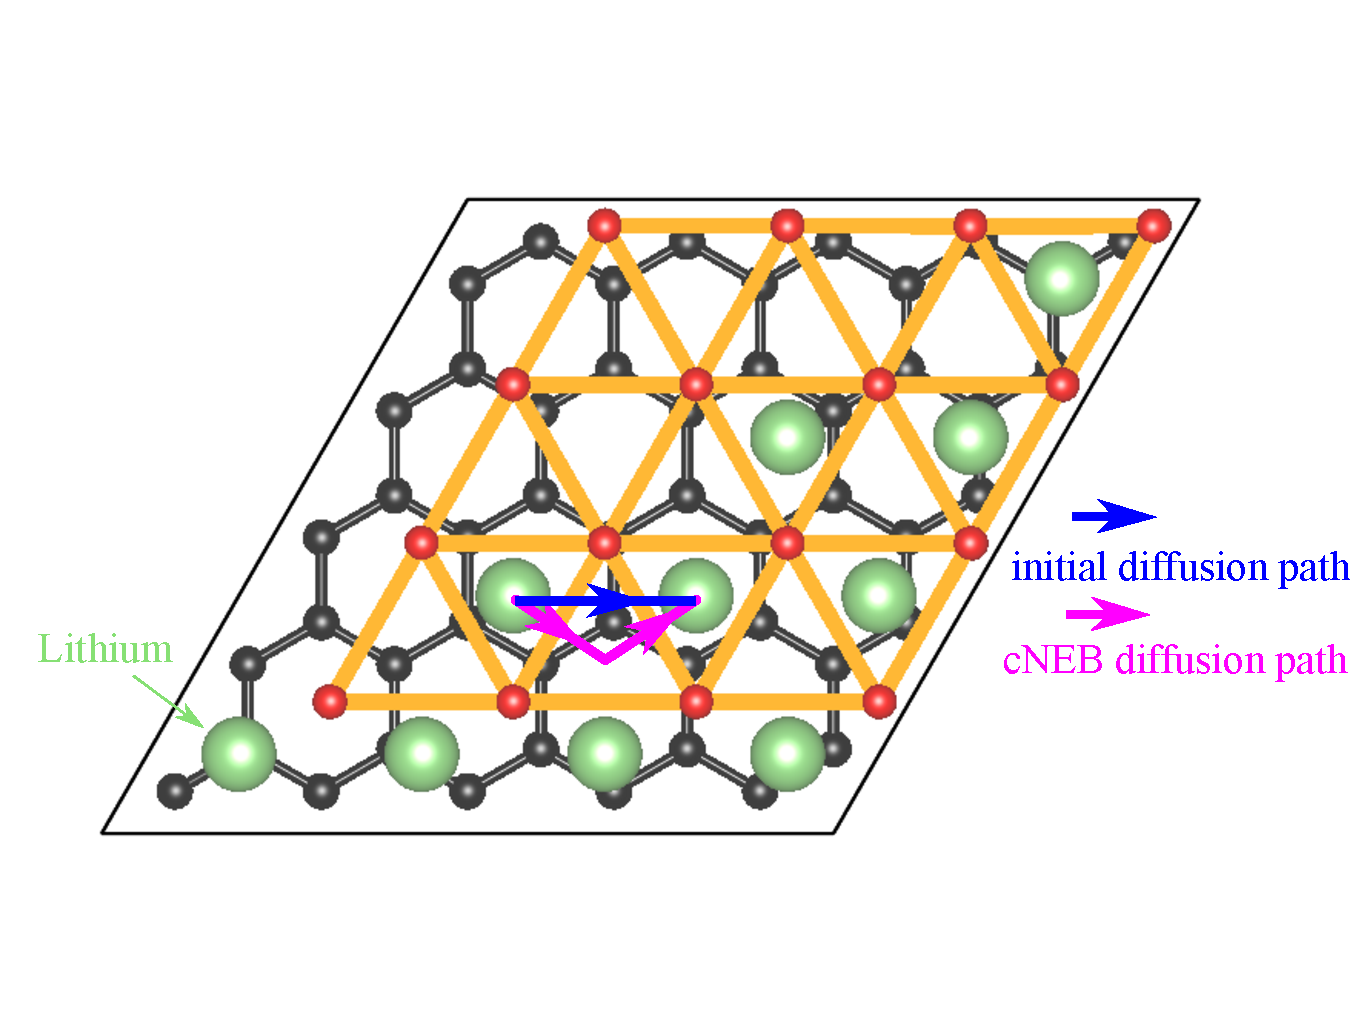
\includegraphics[width=0.7\linewidth]{sites_path.eps}%
\caption{Initial guessed and final resulted Li diffusion path between Ti$_2$CO$_2$+Gr heterostructure. }
\end{figure}

\begin{figure}[htbp]
\centering
\includegraphics[width=0.7\linewidth]{path.eps}%
\caption{Top and side view of  the lowest energy diffusion path of Li in Ti$_2$CO$_2$ related systems. \label{path}}
\end{figure}

\begin{figure}[htbp]
\centering
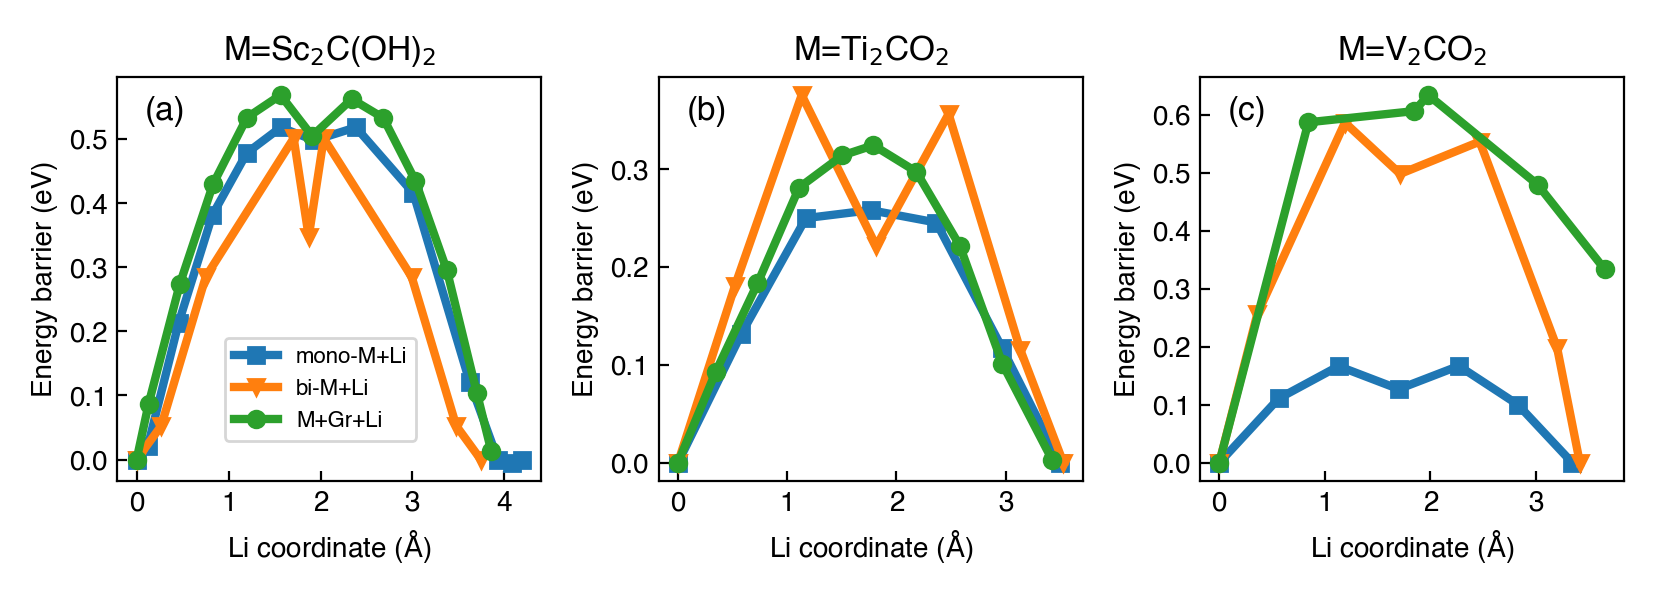
\includegraphics[width=0.6\linewidth]{Li_barrier.png}%
\caption{Energy profiles of  Li diffusion in different systems composed of (a) Sc$_2$C(OH)$_2$, (b) Ti$_2$CO$_2$ and (c) V$_2$CO$_2$ along the lowest energy diffusion path as indicated in \autoref{path}. \label{barrier}}
\end{figure}

A low diffusion barrier and high mobility are the requirements of an efficient electrode material. In particular, the mobility of a metal atom on an electrode material is a key factor determining the rate performance during charging and discharging of a battery. Following the thermodynamic consideration of Li intercalation, we investigated the single Li kinetics on mono-M+Li, within bi-M+Li and within M+Gr+Li heterostructures, where M=Sc$_2$C(OH)$_2$, Ti$_2$CO$_2$ and V$_2$CO$_2$, by calculating the lowest energy Li atom diffusion path connecting two adjacent binding sites using the cNEB method, see \autoref{path}. The determined energy profiles of the paths are shown in \autoref{barrier}. Compared to the bilayer systems, Li displays relatively smaller diffusion barriers on the pristine monolayers. In other words, energy barriers of Li ions in a M$_2$CX$_2$+Gr+Li heterostructure are always higher than those of monolayers. For instance, while the energy barrier is calculated to be 0.16 eV on mono-V$_2$CO$_2$+Li, it becomes 0.6 eV for bi-V$_2$CO$_2$+Li and V$_2$CO$_2$+Gr+Li heterestructure. Since the multilayer system has the advantage of having higher capacity than the single monolayer system for given volume, and also the synthesized M$_2$CX$_2$+Gr will mostly be multilayered, we believe that the monolayer structures represent the lower limit for the energy barriers. However, to obtain realistic kinetics properties we should consider the diffusion of ions between layers not only on isolated monolayers. Another important point is that surface functionalization increases the barrier considerably\cite{doi:10.1021/jp504493a}. Interestingly, energy barriers for Ti based systems are similar, varying in the range of 0.22-032 eV.  Our calculated energy barriers for mono-Ti$_2$CO$_2$+Li are consistent with a recent work\cite{doi:10.1021/jp504493a}. Energy barriers for Ti-based systems are lower than that of graphite 0.5 eV\cite{Thinius2014} and high-capacity bulk silicon anode materials with a diffusion barrier around 0.57 eV, comparable to the commercially used anode materials based on TiO$_2$ which have a barrier of 0.35-0.65 eV\cite{tio2-barrier,tio2-barrier-4,tio2-barrier-3}, suggesting that heterostructures of Ti-based MXenes with graphene are promising candidates for electrode materials in battery applications. The diffusion barriers can be reduced by weakening the interaction of Li ions with the constituent layers. This can be achieved by fabricated pillar structures in which the interlayer distance of graphene and MXenes is enlarged by the help of intercalated molecules \cite{Luo2017}. This method can also improve the storage capacity by multilayer absorption between the layers. 



\subsection{Summary}
We carried out first-principles calculations to systematically investigate Li atoms intercalation in MXenes/graphene vertical bilayer heterostructures for Li battery application. Six members in the MXenes family were considered to form heterostructures with graphene: M$_2$CX$_2$+Gr (where M=Sc, Ti, V and X=OH, O). The ground state stacking types of bilayer and the strongest binding sites of Li atoms were first determined. The strength of the binding of the bilayer heterostructure is comparable to that of bilayer graphene, and is stronger than for MXenes bilayers. Due to a finite mismatch of the lattice constant of MXenes and graphene, the relative motion of the bilayer in the heterostructure require less energy as compared with the other two cases and give a low friction between them.

We identified two promising heterostructure for Li intercalation: Ti$_2$CO$_2$+Gr and V$_2$CO$_2$+Gr. The stability of the heterostructure upon Li intercalation is confirmed through; 1) small variations of the structural parameters , e.g. in-plane lattice parameters ($<$1\%) and interlayer separation ($<$0.5 {\AA}); 2) Large negative binding energies of Li atoms, e.g. larger than that in bilayer graphene; 3) Li atom donates a significant amount of charge to the host material and exists in the cationic state. We found that all the possible Li absorption sites can be occupied without destroying stability, namely 100\% Li intercalation, leading to an average open circuit voltage of 1.49 V for Ti$_2$CO$_2$+Gr and 1.93 V for V$_2$CO$_2$+Gr. Especially, Ti$_2$CO$_2$ MXene offers a compromise between capacity and kinetics since the calculated diffusion barriers are the lowest among the other considered systems and which is lower than that of graphene.  A balance between the storage capacity and kinetics should be made for practical applications  when selecting a promising candidate. Due to their lower molecular weights as compared to bare MXenes bilayers,  MXene+Gr heterostructure offer higher storage density, they also have the advantage of good electrical conductivity which is an essential property for a proper operation of a battery. 
%!TEX root = ../thesis.tex
%*******************************************************************************
%****************************** Second Chapter *********************************
%*******************************************************************************

\chapter{Results of Physical Properties Modification in Novel 2D materials \label{chap:5}}

\ifpdf
    \graphicspath{{Chapter5/Figs/Raster/}{Chapter5/Figs/PDF/}{Chapter5/Figs/}{Chapter5/Figs/Vector/}}
\else
    \graphicspath{{Chapter5/Figs/Vector/}{Chapter5/Figs/}}
\fi

This is the second part of the results of this thesis. Here we will discuss some of the possible ways to modify the physical properties of 2D materials. As before, each section will be focused on an unique way to change the properties of materials, namely number of layers, mechanical strain, heterostructure and defect induction. Following the theme of the thesis, which is about novel 2D materials, we will continue to introduce other new 2D that has been discovered and whose properties will be modified. 

\section[Number of layers: Few-layer of Calcium hydroxide]{Number of layers: Few-layer of Calcium hydroxide \footcite[This work is published in:][]{Aierken2015.porlandite} \label{CaOH2_layers}}

\subsection{Introduction}

We have seen several monolayer systems that exacted from layered materials such 2D-BN, 2D-MoS$_2$, in this work, we further explore this process for alkaline earth metal hydroxides (AEMHs), which pose a layered structure in the bulk form. It was exfoliated  to few-layer, the experiment and the theoretical modelling is reported in this section. In contrast to the abundant literature on graphenelike ultra-thin structures, few-layer AEMHs have not been investigated so far. Bulk forms of AEMHs are layered structures belonging to the $P\overline{3}m1$ space group\cite{structure1} and the crystal structure of a layered AEMHs comprises stacked sheets of MO$_6$ (M=alkaline earth metals) edge-sharing octahedra, see \autoref{fig:str_caoh2}. At each corner of an octahedron, each O atom binds one H atom and the latter interacts with three neighboring hydroxyl groups of the adjacent layer. Early studies on bulk AEMHs revealed that the application of temperature and pressure may result in dramatical changes in their crystal structure and their electronic properties\cite{amorphization1,amorphization2,amorphization3,amorphization4,transition1,transition2,transition3,transition4} . Moreover, early theoretical studies showed the reliability of the use of first principle calculations with a plane-waves basis set in combination with the GGA exchange-correlation functional for the investigation of structural and electronic properties of these materials\cite{Winkler1995,Baranek2001,Azuma2011,DArco1993}.

\begin{figure}
\centering
\includegraphics[width=0.8\textwidth]{str_caoh2.eps}
\caption{\label{fig:str_caoh2} Atomic structure of bulk Ca(OH)$_2$: (a)
tilted view, (b) top view of one layer. }
\end{figure}

Although the structural and electronic properties of bulk AEMHs have been
investigated before \cite{Azuma2011,Pishtshev,Pishtshev1} , single layers of 
these materials have never been studied before and their stability is 
still an open question. However, advances 
in experimental techniques made exfoliation and growth of such 
structures possible\cite{new1,new2}. Especially the Portlandite material, Ca(OH)$_2$,
which has been the 
main product of hydration of Portland cement, CaO, is one of the most well-known 
AEHMs, characteristic properties of ultra-thin structures of Portlandite have 
not been reported yet. In this study we investigate, both experimentally and theoretically, 
the structural, electronic, magnetic, vibrational and mechanical 
characteristics of bulk, bilayer and monolayer Ca(OH)$_{2}$ and discuss how these properties change with the number of layers.  Particularly, the result of the phonon calculation is presented for the confirmation of the stability of the newly proposed 2D material.

To assess the mechanical strength of the material, in addition to the elastic moduli that we have introduced in \autoref{chap:3}, here we calculate another useful parameter that closely related to the Young's modulus, which is called the in-plane stiffness of the materials. We 
focused on the harmonic range of the elastic deformation, where the structure 
responded linearly to strain $\epsilon$. The stretching of the Ca(OH)$_{2}$ is 
achieved by increasing the equilibrium lattice constant a$_{0}$ by $\Delta$a, 
to attain the axial strain $\epsilon$ = $\Delta$a/a$_{0}$. We optimized the 
atomic structure at each increment of the strain, $\Delta\epsilon$ =0.01 and 
calculated the total energy under strain E$_{T}$($\epsilon$). Then the strain 
energy can be given by, E$_{S}$ = E$_{T}$($\epsilon$) - E$_{T}$($\epsilon$=0); 
namely, the total energy at a given strain $\epsilon$ minus the total energy at 
zero strain. Then, using the following formula, one can calculate the in-plane 
stiffness: 
\begin{equation}
 C = (\dfrac{1}{A_{0}})(\dfrac{d^{2}E_{S}}{d\epsilon^{2}}),
\end{equation}
where A$_{0}$ is the equilibrium area of the supercell.

As explained in detail in the following sections, unitcells including one Ca,
two O and two H are the primitive cells of both monolayer and bulk structures, 
it is doubled for bilayer. Cohesive energy per unit cell,
$E_{coh}$ is presented in \autoref{tab:str2_caoh2} and is calculated according to the formula:
$E_{coh}=E_{tot}-nE_{Ca}-2nE_O-2nE_H$, where $E_{tot}$ is the total energy
of the unit cell of Ca(OH)$_2$, $E_X$ is the single atom total energy of atom $X$
and $n$ is the number of Ca atoms for the corresponding unit cell, i.e.
$n=1$, $n=2$ and $n=1$ for monolayer, bilayer and bulk, respectively. 

\subsection{Computational details}

\begin{footnotesize}
\begin{description}
\item[Simulation program:] VASP and PHON\cite{alfe}
\item[Energy cut-off:] 500 eV
\item[Pseudopotentials:] PBE-GGA(PAW)
\item[k points (Monkhorst-Pack):] 35$\times$35$\times$1 and 25$\times$25$\times$11 for few-layer and bulk Ca(OH)$_{2}$, respectively 
\item[Vacuum:] 25~\AA
\item[Energy and force convergence criterion:] 10$^{-5}$ eV and 10$^{-2}$ eV/\AA, respectively
\item[vdW corrections:] DFT-D2 method of Grimme \cite{Grimme}
\item[Charge analysis:] Bader's charge analysis method\cite{Bader1,Bader2,Bader3}
\end{description}
\end{footnotesize}



\subsection{Experimental measurements}


Before our theoretical investigation of few-layer Ca(OH)$_{2}$, first we 
present the experimental realization and detailed theoretical analysis of the
characteristics of bulk Ca(OH)$_{2}$ crystals.


\begin{figure}[htbp]
\centering
\includegraphics[width=0.6\textwidth]{exp_caoh2.eps}
\caption{\label{fig:exp_caoh2} (a) Optical image of the crystal structure and (b) Raman 
spectrum measured using 488 nm laser in the low and the high frequency region. 
The fundamental phonon branches located at the low frequency (100-400 cm$^{-1}$  range) and the high frequency (~3620 cm$^{-1}$) are associated with the OH  stretching mode. (c) XRD measurements}
\end{figure}

Ca(OH)$_{2}$ crystals were grown using the hydrolysis technique by using 
Ca$_{3}$SiO$_{5}$ micro-pallets. Ca$_{3}$SiO$_{5}$ was mixed at different water 
to solid ratios ranging from 0.2 to 0.9 by molar weight. The mixture was heated 
up to 40 $^{\circ}\mathrm{C}$ in a controlled reaction chamber for 3 hours and 
controllably cooled down to 5 $^{\circ}\mathrm{C}$ for 24 hours using a
temperature controller. The growth time depends on the total water to solid 
ratio as well as the growth temperature. Growth time was around 8 hours for 0.6 
water to solid ratio and 40 $^{\circ}\mathrm{C}$ growth temperature. 
Longer growth time typically resulted in a dendritic morphology where the 
growth was mostly in the c-axis direction. Synthesized crystals displayed rather sharp (FWHM ~ 7 cm$^{-1}$) Raman feature at 280 cm$^{-1}$ and our XRD measurements displayed sharp (00l) reflections at 19.1, 39, 56.2, 77.7 degrees implying that crystals have lamellar nature.  
 

Synthesized crystals were around 0.1-2 mm in size and they 
were filtered from the solution. After the filtering process, crystallites were 
washed off using 18.2 MOhm.cm DI wafer multiple times and dried under inert Ar 
gas. Crystallites were exfoliated using micro-mechanical exfoliation technique 
onto thermal silicon oxide / Si substrates. We find that the contrast 
was improved for an oxide thickness around 265-285 nm.
Exfoliated flakes displayed rather sharp edges (see \autoref{fig:exp_caoh2}) with 
well-defined angles of 120\textdegree ~and 60\textdegree ~implying that the 
materials are highly crystalline. Interestingly, synthesized Ca(OH)$_{2}$ flakes 
are layered in agreement with theoretical calculations and these flakes can be 
easily exfoliated using the Scotch tape technique on different substrates. 
The exfoliated flakes do not show any signs of structural imperfection, pit 
formation, and overall rather flat surfaces can be obtained. In \autoref{fig:exp_caoh2}, the 
yellowish looking regions actually correspond to regions where the thickness is 
around 50-100 nm (50-100 layers) while the blue features are only 10-50 nm in 
thickness. Considering the ease to exfoliate this material, experimentally and 
theoretically we predict that they can be eventually isolated down to mono- and 
few-layers on various substrates.

In addition, micro-Raman measurements were performed using a 488 nm laser on a 
2 micron square spot using a high intensity laser of 10 mW. We noticed that 
few-layers of Ca(OH)$_{2}$ were not subject to local over-heating / 
decomposition effects unlike TMDs (MoS$_2$, 
WS$_2$, etc.) which typically decompose around 100 microWatt power using a 
similar laser excitation spot. We attribute this to the low absorption of the 
material associated with the rather large band gap. Raman measurements 
displayed various peaks in the 100-1000 cm$^{-1}$ range. The high frequency peak 
at 3620 cm$^{-1}$ is associated with the O-H stretching mode $A_{1g}$. In 
addition, the low frequency $E_u(T)$ mode is found at 280 cm$^{-1}$.  

Here, we note that even though this material is a direct gap semiconductor, 
their band gap is well beyond our detectors range and since the insulators 
cannot be excited with such high laser wavelength, PL measurements are 
virtually impossible.

\subsection{Structure properties}\label{strcuture}

The bulk structure of Portlandite is formed by the stacking of individual Ca(OH)$_2$ monolayers on top of each other, see \autoref{fig:str_caoh2}. As we will exam and discuss the stacking in detail in the following paragraphs, we learned that the AA stacking is the ground state atomic configuration for bulk and multilayer structures of Ca(OH)$_2$. In \autoref{tab:str_caoh2}, optimized lattice parameters of the bulk structure together with experiments and other theoretical calculation are presented. Our results consist with reference \cite{Pishtshev} and together they have good agreement with experiments. This justify the reliability of our calculations. 

In the 5-atomic hexagonal primitive unit cell of bulk Ca(OH)$_2$, the Ca atom sits at the geometrical
center of the cell, i.e. $\left\lbrace 1/2a, 1/2b,
1/2c \right\rbrace$. Two O and two H atoms form two hydroxyl groups 
(-OH$^-$) located symmetrically with respect to the Ca atom. In this 
arrangement, coordinates of H and O only differ by their positions along the 
\textbf{c} lattice axis and their fractional coordinates can be given as
$\left\lbrace1/6a, 1/6b, (1/2c-c_O) \right\rbrace$ and $\left\lbrace 
1/6a, 1/6b, (1/2c-c_H) \right\rbrace$ for one hydroxyl,
$\left\lbrace 5/6a, 5/6b, (1/2c+c_O) \right\rbrace$
and $\left\lbrace 5/6a, 5/6b, (1/2c+c_H)
\right\rbrace$ for the other one, where c$_O$ and c$_H$ are the vertical shifts
of the positions of O and H atoms from the Ca plane in the unit of \AA~, respectively. 

\begin{table}
\centering
\caption{\label{tab:str_caoh2}
Comparison of calculated results for structures parameter of bulk Ca(OH)$_2$ with experimental results and with theoretical results from other reference: lattice constants 
$a$ and $c$, volume $V$ and $c/a$ ratio. }
\begin{threeparttable}
\begin{tabularx}{0.92\linewidth}{X|XXXX}
\hline\hline
Structure parameters & Exp. \tnote{a} & Exp. \tnote{b} & PBE-PAW (this work) & PBE-PAW \tnote{c}  \\
\hline

$a$ (\AA)                   & 3.589 & 3.592 & 3.614 & 3.612 \\
$c$ (\AA)                   & 4.911 & 4.906 & 4.982 & 4.942 \\
$V$ (\AA$^3$)               & 54.78 & 54.82 & 56.35 & 55.85 \\
$c/a$                       & 1.368 & 1.366 & 1.379 & 1.368 \\

\hline\hline

\end{tabularx}
\begin{tablenotes}
\begin{footnotesize}
\item[a]Ref. \cite{exp.1}
\item[b]Ref. \cite{exp.2}
\item[c]Ref. \cite{Pishtshev}
\end{footnotesize}
\end{tablenotes}
\end{threeparttable}
\end{table}

In the optimized structure, the lattice constants $a$ and $c$ are 3.61 \AA~and 4.98 \AA~in the bulk structure, parameters c$_O$ and c$_H$ are calculated to be 1.15 \AA~and 2.12 \AA . Bond length of Ca-O and O-H are 2.36 \AA~ and 0.97 \AA . Interlayer distance which is defined as the distance between the uppermost H-layer of the underlying layer and the lowermost H-layer  of the top-lying layer is found to be 0.49 \AA~. Differing from other lamellar bulk crystal structures such as graphite (3.58 \AA) and MoS$_{2}$ (3.42 \AA)\cite{can} , Ca(OH)$_{2}$ layers are more closely stacked on top of each other. 

Our calculations revealed that going from bulk to monolayer the in-plane lattice parameter $a$ change to 3.62 \AA~. In our calculations, the c lattice parameter in the hexagonal unit cell of the monolayer is set to 25 \AA~in order to avoid interlayer interaction between the adjacent layers. In the monolayer Ca(OH)$_2$, parameters c$_O$ and c$_H$ are calculated to be c$_O$=1.14 \AA~and c$_{H}$=2.10 \AA~, respectively. Ca-O and O-H bond distances are 2.38 \AA~and 0.97 \AA~in the monolayer, respectively. We observed only quite small change as the system going from bulk to monolayer, some of the structure parameters even left unchanged, from this we can conclude quite weak interlayer interaction in Ca(OH)$_2$. In order to study the interlayer interaction we further investigate their effect on stacking, and by including the vdW correction in the functional we are able to identify the nature of this interaction.

\begin{table}
\centering
\caption{\label{tab:str2_caoh2}
Calculated results for different structures of Ca(OH)$_2$: lattice constants 
$a$, vertical shift of O and H atom c$_O$ c$_H$, Ca-O and O-H bond length, energy band gap $E_{gap}$, cohesive energy 
per atom $E_{coh}$, charge transfer from Ca atom to O atom $\Delta Q$, in-plane Young's modulus 
$E_{xx},E_{yy}$, in-plane Poisson's ratio $\nu_{xy}$, in-plane shear 
modulus $G_{xy}$ and in-plane stiffness $C$. For comparison, theoretical calculation on same quantities of BN are shown in the last row.}
\begin{threeparttable}
\adjustbox{max width=\textwidth}{%
\begin{tabular}{l|llllllllll}
\hline\hline
System & $a$ & c$_O$/c$_H$ & Ca-O/O-H & $E _{gap}$ & $E_{coh}$ &  $\Delta Q$ &
$E_{xx},E_{yy}$ &  $\nu_{xy}$ & $G_{xy}$ & $C$\\
& (\AA) & (\AA/\AA) & (\AA/\AA) & (eV)& (eV) & (e) & (N/m) &  & (N/m) & (J/m$^{2}$)\\
\hline

\textbf{Bulk Ca(OH)$_{2}$} & 3.61  & 1.15/2.12 & 2.36/0.97 & 4.08 & 4.52 & 1.6 
& 55.0 & 0.30 & 21.23 & 60.1\\
\textbf{2L Ca(OH)$_{2}$}   &3.62& 1.15/2.12 & 2.38/0.97 & 3.70 & 4.48 & 1.6 & 50.7 & 0.32 & 19.16 & 55.6 \\
\textbf{1L Ca(OH)$_{2}$}   &3.62& 1.14/2.11 & 2.38/0.97 & 3.67 & 4.39 & 1.6 & 50.7 & 0.33 & 19.08 & 53.2 \\
\textbf{1L BN}             &2.51\tnote{a}& - & 1.45\tnote{a}~~\tnote{b} & 4.64\tnote{a} & 8.82\tnote{a} & 0.43\tnote{a}~~\tnote{c} & 278.2\tnote{d} & 0.22\tnote{d} & 113.5\tnote{d} & 267\tnote{e} \\
\hline\hline
\end{tabular}}
\begin{tablenotes}
\begin{footnotesize}
\item[a]Ref. \cite{Topsakal} 
\item[b]B-N bond length
\item[c]charge transfer from B to N
\item[d]Ref. \cite{Peng}
\item[e]Ref. \cite{silicene-prb}
\end{footnotesize}
\end{tablenotes}
\end{threeparttable}
\end{table}


Individual layers of lamellar structures such as graphite, hex-BN and TMDs 
are held together mainly by the vdWs force in order to form a bulk 
layered structure. Such a weak interaction stems from dynamical correlations 
between 
fluctuating charge distributions in neighboring layers. Here we 
investigated the energies of various bilayer configurations. As presented
in \autoref{fig:stack_caoh2} there are six possible types of stacking between two 
Ca(OH)$_2$ monolayers. Similar to the stacking nomenclature of bilayer graphene, 
we classify the stacking types to be either AA or ABn (n=1,2,...,5). The 
same type of atoms from different monolayers are on top of each other in AA 
stacking whereas AB stackings can be reached by shifting one of the layers along 
certain lattice vectors. One set of AB stackings could be realized by shifting 
the second layer in the AA stacking towards [$\overline{1}\overline{1}0$], 
which gives stacking AB1, and by shifting towards the [110] direction, which 
gives stacking AB2, see first row in \autoref{fig:stack_caoh2}. Another set of 
bilayers are achieved by first flipping the second layer upside down in AA 
stacking, which
would gives stacking AB3, then AB4 and AB5 can be constructed by doing the 
same shifting on the second layer of AB3 towards [$\overline{1}\overline{1}0$] 
and [110] directions of the 1st layer, respectively. After relaxation of all 
stackings, the variation of the \textbf{a} lattice constant among the different 
stacking types is less than 0.01 \AA~. The smallest interlayer
distance, as defined previously for bulk, is for AA stacking which equals
0.49 \AA~, the same as that in bulk. For AB
stacking the interlayer distance is 1$\sim$2 \AA ~larger than that for AA
stacking. As depicted in \autoref{fig:stack_caoh2}, AA stacking is 96$\sim$137 meV
per formula more favorable than all other possible stacking types and hence it
corresponds to the lowest energy configuration. 

\begin{figure}[htbp]
\centering
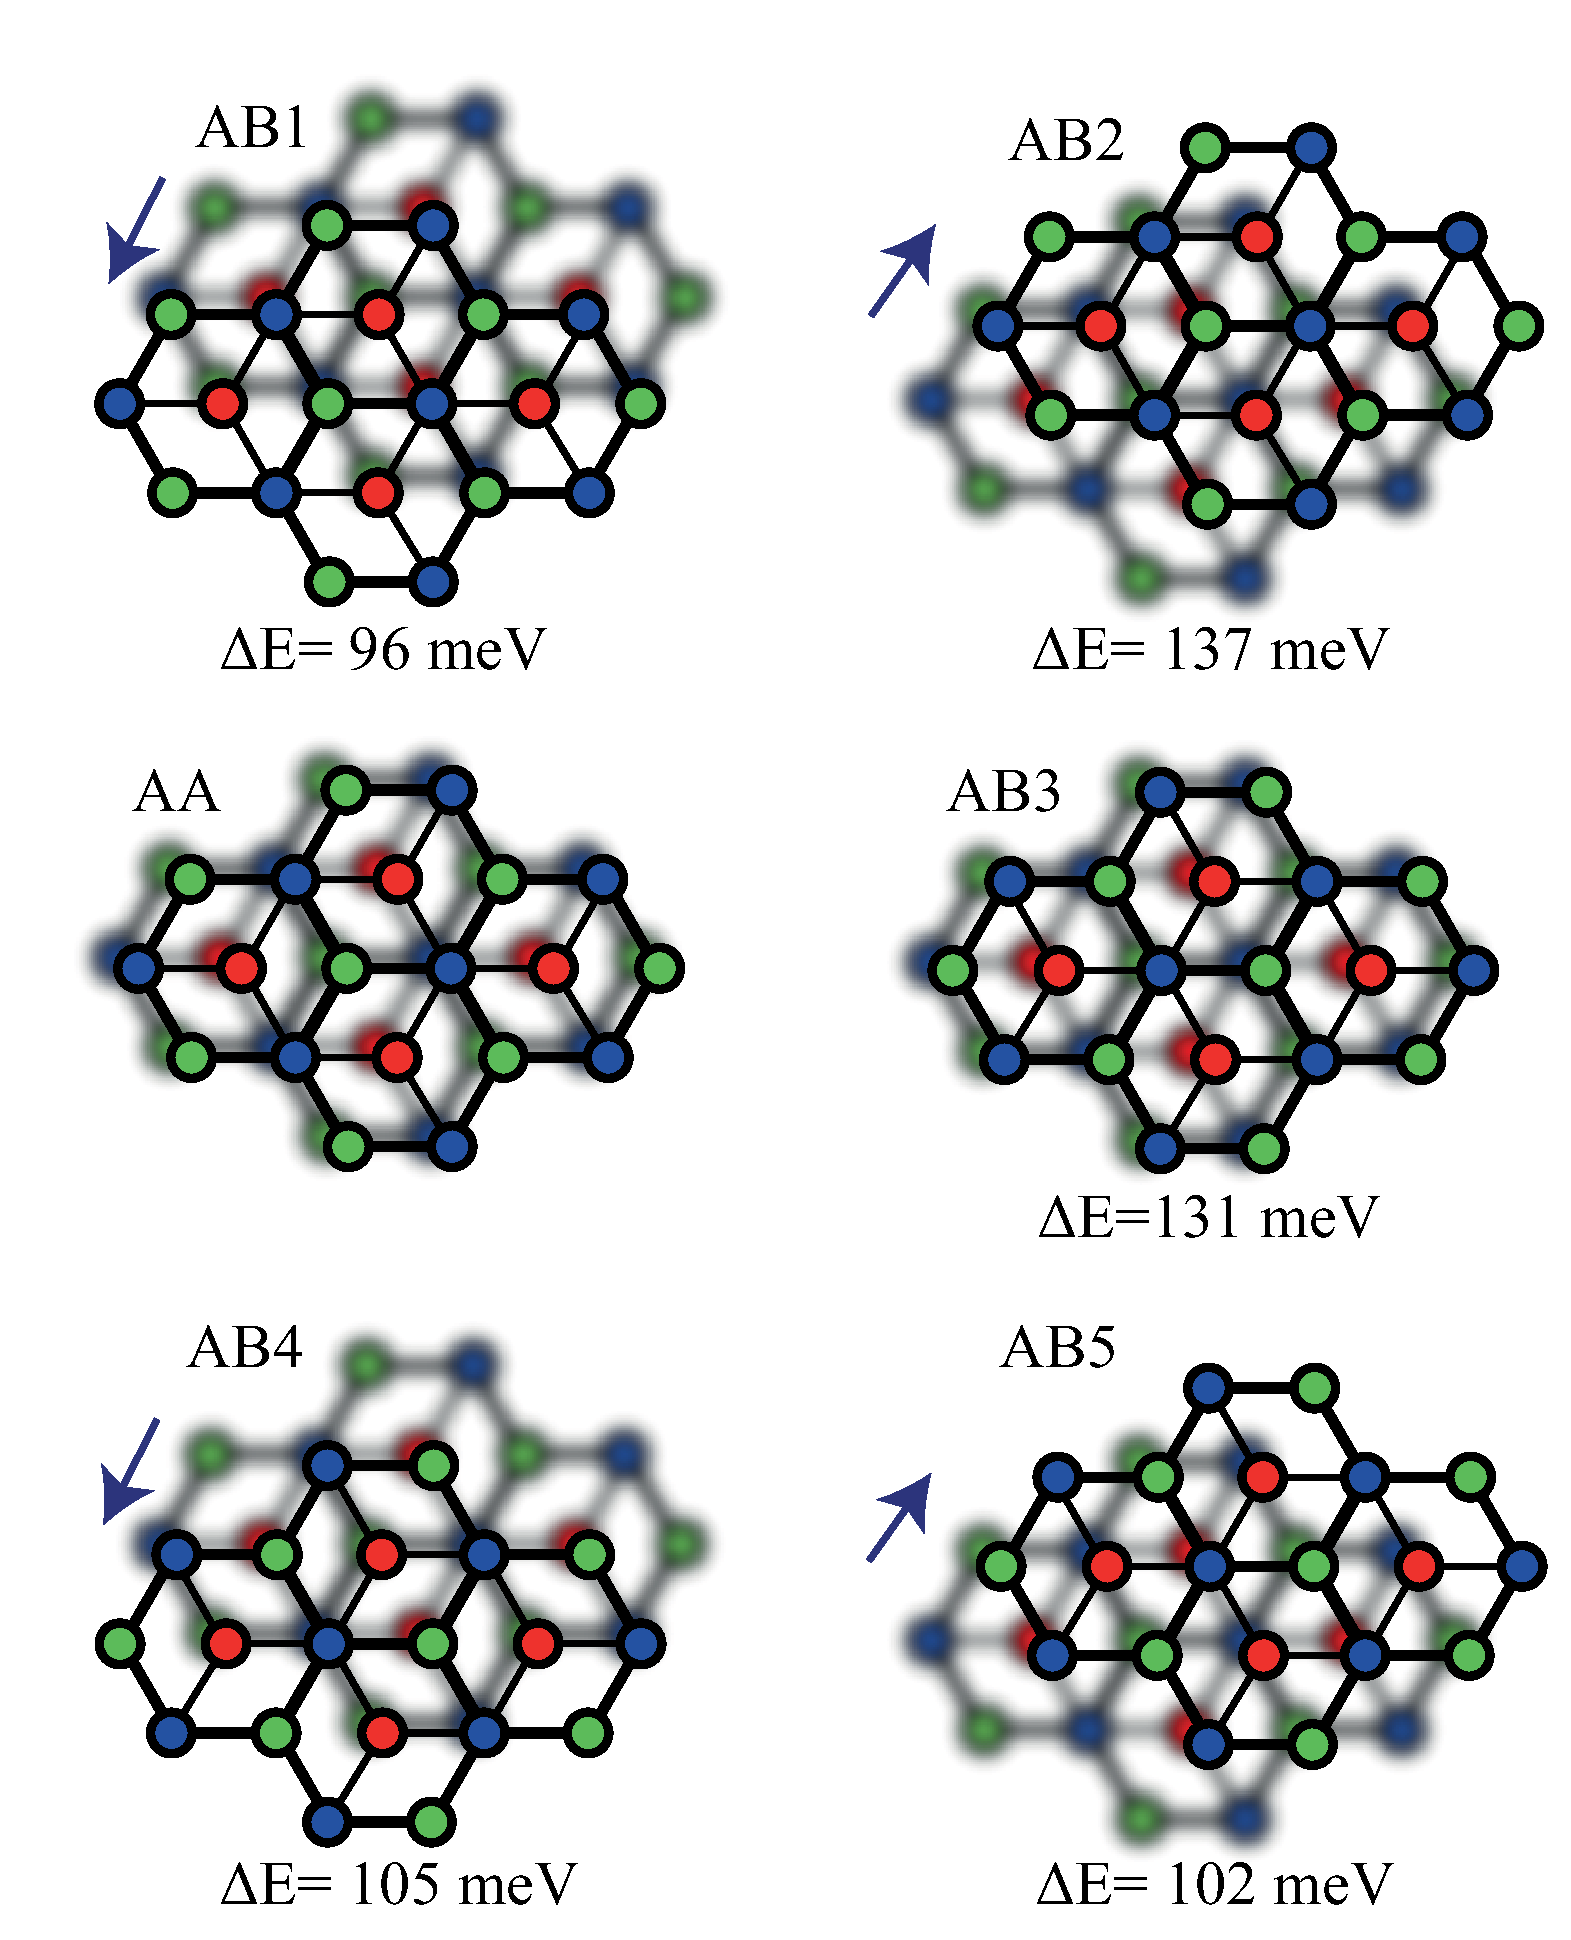
\includegraphics[width=0.8\textwidth]{stack_caoh2.eps}
\caption{\label{fig:stack_caoh2} Different stacked bilayers (bottom layer is blurred)
and their energy difference with respect to the AA stacking of Ca(OH)$_2$, i.e.
$\Delta$E=E$_{\text{ABX}}$-E$_{\text{AA}}$, (X=1,2,...,5). Energies are given
per formula of Ca(OH)$_2$. Blue, green and red circles are for Ca atom, 
upper hydroxyl group and lower hydroxyl group, respectively. For clarity, the 
bottom layer is shifted slightly.}
\end{figure}

\begin{figure}[htbp]
\centering
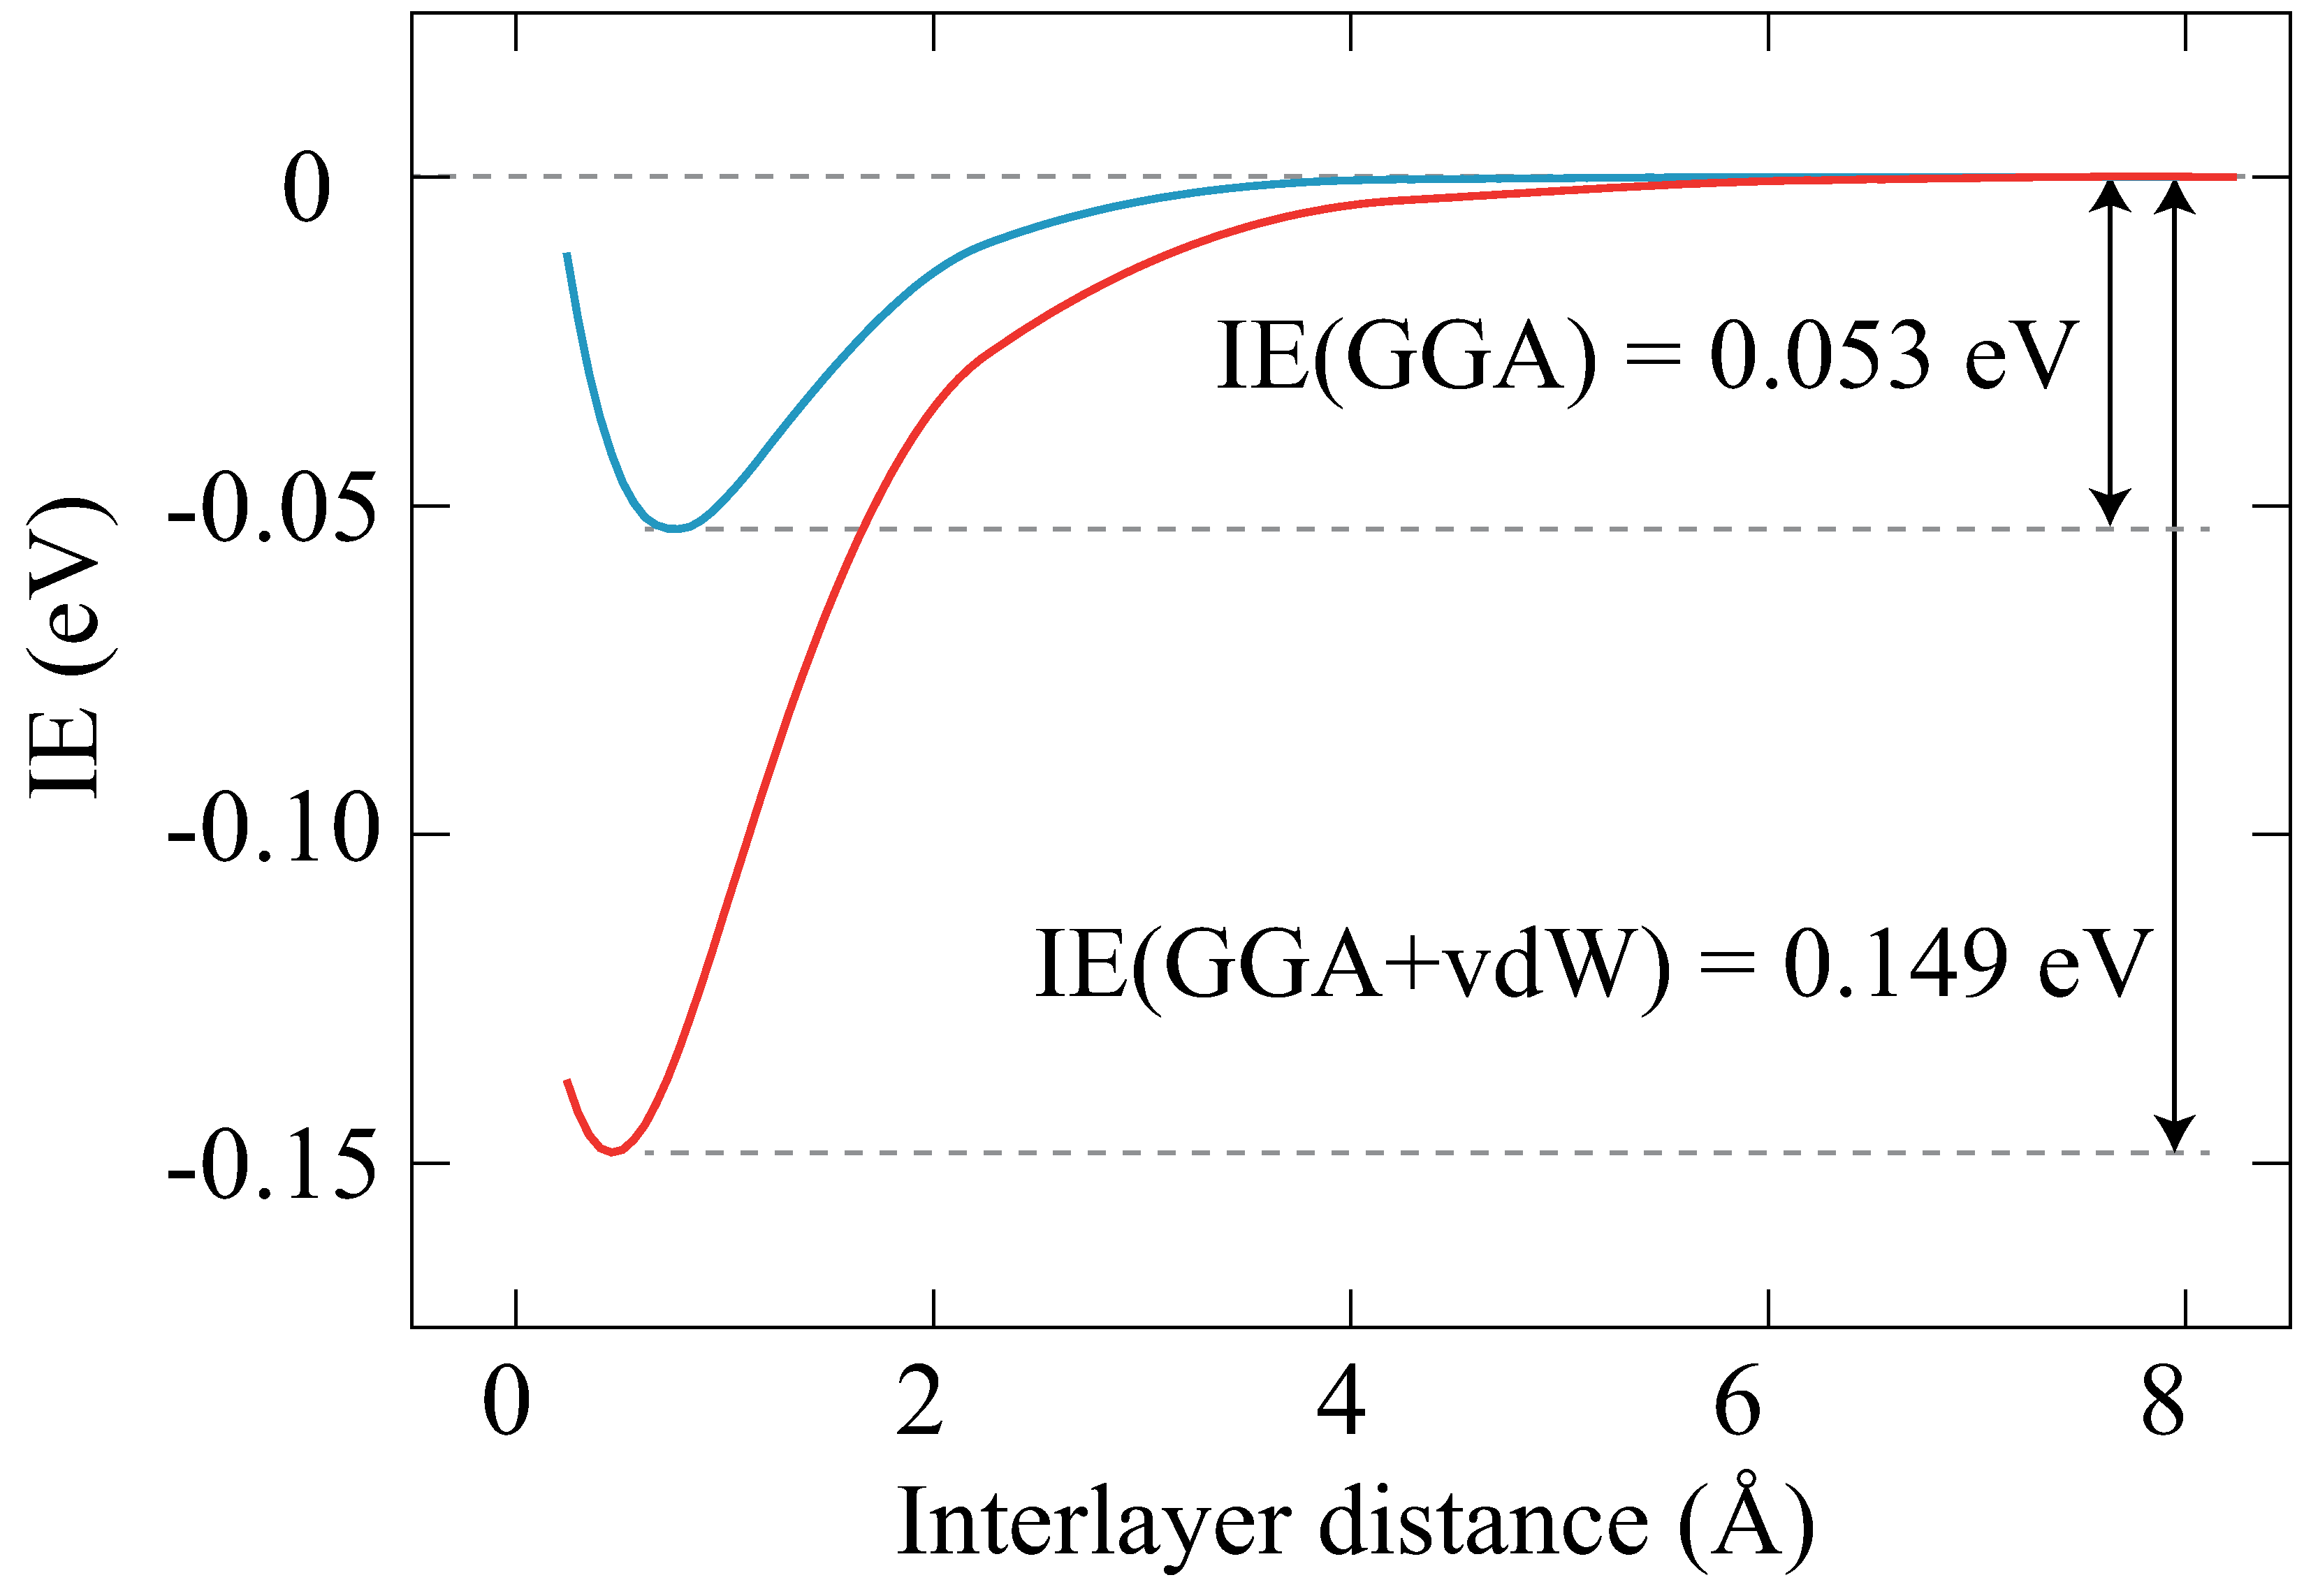
\includegraphics[width=0.8\textwidth]{int_caoh2.eps}
\caption{\label{fig:int_caoh2} Interlayer interaction energy per formula of
AA-stacked bilayer Ca(OH)$_2$. Blue and red curves are for GGA calculations
without and with vdW correction, respectively.}
\end{figure}

To investigate the nature of the interlayer interaction, we 
have calculated the interlayer interaction energy (IE) for the AA stacked 
bilayer structure of Ca(OH)$_2$. The IE is the energy difference between the 
total energy at a specific interlayer distance and that of a well
separated bilayer. The plot of IE versus interlayer distance is shown in \autoref{fig:int_caoh2}, where the energy of the  well separated bilayer is defined as 
0 eV. Two sets of calculations were performed, one set only considers GGA 
exchange correlation; while another set considers both the GGA and vdW 
interaction. At the optimized interlayer distance for the bilayer structure, 
almost 2/3 of the attractive interaction comes from the vdWs 
interaction, and this is consist with \citet{DArco1993} . They stated that
interlayer interaction of Brucite, one of the isomorphous of Portlandite, is
mainly a dispersion-type interaction. The nature of interlayer interaction in Ca(OH)$_2$ is mainly vdW type weak interaction. Our GGA+vdW calculations revealed that the interlayer interaction between two layers of Ca(OH)$_2$ (149 meV per formula) is much stronger than that of bilayers of MoS$_2$ (76 meV per formula).


\subsection{Electronic properties}\label{sec:electronic}

\begin{figure}[htbp]
\centering
\includegraphics[width=0.7\textwidth]{elec_caoh2.eps}
\caption{\label{fig:elec_caoh2} (a) and (d) are the Band structures, 
(b) and (e) are the partial DOS and (c) and (g) are the band and $k$-point decomposed charge densities of the bulk (c) and monolayer (g) Ca(OH)$_2$, respectively. The charge density are the band edges indicated in (a) and (d), isovalues are kept constant. (f) Band structure around $\Gamma$ point is shown with (dashed line) and without (solid line) spin orbit coupling. }
\end{figure}

Our Bader charge transfer analysis showed that the final (initial) electron 
charge on Ca, O and H atoms after (before) the formation of the crystal are 
6.4$e$ (8.0$e$), 7.4$e$ (6.0$e$) and 0.4$e$ (1.0$e$), respectively. Therefore, 
in the bulk structure of Ca(OH)$_2$, Ca-O bonds, which are 
mostly in ionic character, are formed through 0.8$e$ charge transfer 
from each Ca to O atom.  Charge transfer is kept unchanged when it comes to the monolayer structure, except for the rest charge on H atom is 0.6$e$ in monolayer.

Our calculations on the electronic structure reveal that bulk Ca(OH)$_2$ is 
an insulator with a 4.37 eV direct band gap. As shown in \autoref{fig:elec_caoh2} (a), the VBM and the CBM are located at the $\Gamma$ point. The partial density of 
states (DOS) shown in \autoref{fig:str_caoh2} (b) indicates that the major 
contribution to the states at the valence and conduction band edge originates 
from the O atoms, while deeper in the conduction band, states are mainly composed 
of the orbitals of Ca. The orbital character of a state at a particular band can 
also be deduced from a band and $k$-point decomposed charge density. As seen 
from \autoref{fig:elec_caoh2} (c), edges in the top of VBM have O-$p_x$ 
and O-$p_y$ orbital character, and the hybridization of these states are also 
shown in the same figure. While the CBM has some $p_z$ orbital 
character from the O atoms, but as the energy of the state increases, the $d$ 
orbitals from Ca atom start to contribute, see \circled{8} in the same figure.

Electronic properties of Ca(OH)$_2$ are quite different from similar
2D graphene-like structures. Unlike TMDs (such as MoS$_2$ and
WSe$_2$) that exhibit indirect-to-direct band gap crossover when going
from bulk to a single layer structure, Ca(OH)$_2$ is a direct band gap
semiconductor which is independent of the number of layers. Although the energy band gap
at the $\Gamma$ point decreases from 4.03 to 3.67 eV for a monolayer structure,
electronic dispersion of the valence band edge remains almost unchanged, see
\autoref{fig:elec_caoh2} (d). As shown in \autoref{fig:elec_caoh2} (e)  
the conduction states mainly originate from Ca atoms, while the valence states 
are mainly composed of the orbitals of O atoms. 

Our magnetic state analysis shows that unless a defect is formed in/on the 
structure, there is no spin polarization in the ground state of both bulk and monolayer Ca(OH)$_2$. Therefore, Ca(OH)$_2$ is a non-magnetic insulator regardless of its dimension for the structure. 

Moreover, it was seen that the spin-orbit interaction has no 
considerable effect on the bond lengths and the overall electronic dispersion 
(except for a 26 meV splitting in the VBM at the 
$\Gamma$ point, see \autoref{fig:elec_caoh2} (f)). Due to the presence of inversion symmetry of Ca(OH)$_2$, the 
degeneracy of spin-up and spin-down states still remains, this is also confirmed 
by the results of our calculation.

\begin{figure}[htbp]
\centering
\includegraphics[width=0.9\textwidth]{suf_caoh2.eps}
\caption{\label{fig:suf_caoh2} Two lowest conduction band charge density of 
monolayer and bilayer Ca(OH)$_2$ at the $\Gamma$ point.}
\end{figure}

Band and $k$-point decomposed charge density in \autoref{fig:elec_caoh2} are 
kept with the same isosurface level for comparison. However, as we further 
reduced the isosurface level at \circled{4} in (d) and (g) of \autoref{fig:elec_caoh2}, which is the lowest conduction band of the 
monolayer at the $\Gamma$ point: $E_{c1}^{~\Gamma}$, charge density forms a planar 
state parallel to the layer on both sides, see \autoref{fig:suf_caoh2} (a), this
is also the case for the second lowest non-spin-resolved conduction band at the same
$k$-point: $E_{c2}^{~\Gamma}$, see \autoref{fig:suf_caoh2} (b). These two states are 
important due to their unique character and having energy right below ionization energy. Such exceptional states 
having free-electron-like dispersion were reported before\cite{Posternak1,Posternak2} for 
doped graphite. To study the trend in these states, the same states were plotted 
for bilayer Ca(OH)$_2$, see (c) and (d) in \autoref{fig:suf_caoh2}. $E_{c1}^{~\Gamma}$ and $E_{c2}^{~\Gamma}$ have lower energies than ionization energy. Therefore, electrons are still close and bond to both sides of monolayers as seen from charge density. In the case of bilayer, interestingly, these states appear only on one side of bilayer.

\subsection{Mechanical properties}

We present the quantities that describe the mechanical 
properties of Ca(OH)$_2$ in \autoref{tab:str2_caoh2}. 
At first, the in-plane Young's modulus of the bulk structure is calculated. 
Bulk Ca(OH)$_2$ has a in-plane Young's modulus (55.0 N/m) and in-plane shear 
modulus (21.23 N/m). Both these quantities indicating flexible nature to in-plane 
tensile and shear deformation of bulk Ca(OH)$_2$. In addition, bulk Ca(OH)$_2$ has 
an in-plane Poisson's ratio of 0.30.  Additionally, the value of the in-plane 
stiffness for bulk Ca(OH)$_{2}$ is calculated to be 60.1 J/m$^{2}$. 

If we go from bulk to bilayer Ca(OH)$_2$, we see a reduction in either the
in-plane Young's modulus or the in-plane shear modulus, which are 50.7 N/m and 
19.16 N/m, respectively. The in-plane Poisson's ratio on the other hand is 
slightly increased to 0.32 and become more spongy-like as opposite to more 
cork-like character\cite{poisson}. In addition, the in-plane stiffness value of 
bilayer Ca(OH)$_{2}$ is calculated to be 55.6 J$/$m$^{2}$. 

We found that monolayer Ca(OH)$_2$ has a quite low in-plane Young's modulus 
(50.7 N/m) when compared to BN (278.2 N/m). The in-plane Poisson ratio (0.33) 
and the in-plane shear modulus (19.08 N/m) of the monolayer are similar with 
those for bilayer, and for BN, they are 0.22 and 113.5 N/m respectively. The 
calculated values of the in-plane stiffness of monolayer Ca(OH)$_{2}$ is 53.2 
J$/$m$^{2}$. 

\subsection{Vibrational properties}\label{stability}
\begin{figure}[htbp]
\centering
\includegraphics[width=0.7\textwidth]{vib_caoh2.eps}
\caption{\label{fig:vib_caoh2} Phonon dispersion of monolayer Ca(OH)$_2$.}
\end{figure}

Lastly, for the analysis of the vibrational spectrum and further examination of 
the dynamical stability of monolayer Ca(OH)$_2$, we performed a 
calculation of the phonon spectrum using both the first-principles small 
displacement methodology (SDM)\cite{alfe} and density functional perturbation 
methodology (DFPT)\cite{baroni}. Here the non-quadratic dispersion of the 
flexural mode around the zone center is directly related to the insufficient 
FFT grid along the vacuum direction. It is seen from \autoref{fig:vib_caoh2} that 
similar to the Raman shift measurements observed from the bulk crystal 
structure, monolayer material has also high-frequency OH stretching 
modes at 3700-3800 cm$^{-1}$. 

Further analysis of the analysis of phonon 
branches shows that the decomposition of the vibration representation of optical 
modes at the zone center is $\Gamma = 4E_{u} + 2A_{2u} + 4E_{g} + 2A_{1g}$. As 
shown in right panel of \autoref{fig:vib_caoh2} there are four Raman-active phonon 
branches around 240, 350, 390 and 3700-3800 cm$^{-1}$. It is also worth to note 
that differing from other TMD structures having 1T phase, presence of H atoms 
results in existence of two different $E_{g}$ and $A_{1g}$ modes. Here the 
phonon dispersion having real eigenfrequencies in the whole Brillouin Zone, 
which is another indication of the stability of monolayer Ca(OH)$_2$.

\subsection{Summary}\label{disc}

By performing first principle calculations on bulk, bilayer and 
monolayer Ca(OH)$_2$ and experimental confirmation of the bulk crystal 
layered structure, we have predicted several important properties of this 
material and their stability. We found that: (i) Ca(OH)$_2$ crystals are 
environmentally stable and their stable structures can be synthesized by 
experimental methods; (ii) Experimentally, we also demonstrated that Ca(OH)$_2$ 
crystals can be grown in layered form and also be exfoliated on arbitrary 
substrates; (iii) The dimensionality of Ca(OH)$_2$ will not change the 
electronic, structural and magnetic properties qualitatively, nevertheless 
intrinsic mechanical stiffness of each layer will become slightly stiffer as 
the system go from monolayer to bilayer. (iv) Interlayer interaction is mainly 
vdWs dispersion-type force, and
the strength of the interaction is stronger than that of similar layered
materials (e.g MoS$_2$ and graphite). (v) The 
conduction states which have a free-electron-like character may be utilized for 
high-mobility electron transfer. 

We believe that the stable structure and the unique electronic properties of ultra-thin 
Ca(OH)$_2$, predicted for the first time here, will trigger interest in this 
new class of materials. 

\section[Number of layers: Few-layer of pentasilicene]{Number of layers: Few-layer of pentasilicene \footcite[This work is published in:][]{Aierken2016.pentasilicene} \label{pSi_layers}}

\subsection{Introduction\label{intro}}

Recently, a new 2D structure for carbon was proposed, called penta-graphene\cite{Zhang2015}. This crystal is composed entirely of pentagonal rings of C atoms with mixed sp$^2$/sp$^3$ orbital hybridization.  However, the silicon counterpart of this structure, penta-silicene, contains a dynamical instability in its monolayer form. A few attempts have been made to stabilize this new Si structure by hydrogenation\cite{Ding2015} and chemical doping\cite{Li2015b}. 

In the present work, we construct multilayer structures of penta-silicene. We use density functional theory to explore their stability and physical properties. Two types of stacking for the penta-silicene layers are found to give stable few-layer structures. These different stacking types lead to completely different electronic properties since one leads to metallic and the other to semiconducting behavior. Somewhat surprisingly, we found that bilayer penta-silicene has lower formation energy than the most stable hexagonal silicene bilayers. Furthermore, we found that the band gaps of these semiconducting penta-silicene bilayers can be tuned by mechanical strain. We first explore the stability of monolayer penta-silicene and demonstrate its dynamical instability. This forms the motivation to study few-layer systems. Then we investigate different stacking possibilities and the resulting stability. Further, we study their mechanical properties by calculating their elastic constants.  We also compare bilayer penta-silicene to the most stable bilayer hexagonal silicene structures. Lastly, The electronic properties of multilayered penta-silicene are discussed.

\subsection{Computational details}

\begin{footnotesize}
\begin{description}
\item[Simulation program:] VASP and Phonopy
\item[Energy cut-off:] 500 eV
\item[Pseudopotentials:] PBE-GGA(PAW)
\item[k points (Monkhorst-Pack):] 17$\times$17$\times$1 and 23$\times$23$\times$1 for insulating and metallic systems, respectively 
\item[Vacuum:] 20~\AA
\item[Energy and force convergence criterion:] 10$^{-8}$ eV and 10$^{-7}$ eV/\AA, respectively
\item[phonon calculation:] finite displacement method
\item[Supercell for phonon calculation:] $4\times4\times1$ and $3\times3\times2$ for few-layer and bulk systems, respectively
\item[\textit{Ab initio} molecular dynamics:] Parrinello-Rahman (NpT) dynamics \cite{vasp_npt1,vasp_npt2} and a Langevin thermostat \cite{vasp_Lgv}
\item[\textit{Ab initio} molecular dynamics (Energy cut-off):] 300 eV
\item[\textit{Ab initio} molecular dynamics (time step):] 2 fs
\item[\textit{Ab initio} molecular dynamics (temperature):] 100 K
\item[\textit{Ab initio} molecular dynamics (simulation time):] 6 ps
\end{description}
\end{footnotesize}

\subsection{Monolayer pentasilicene}\label{mono}

\begin{figure}[htb]
\centering
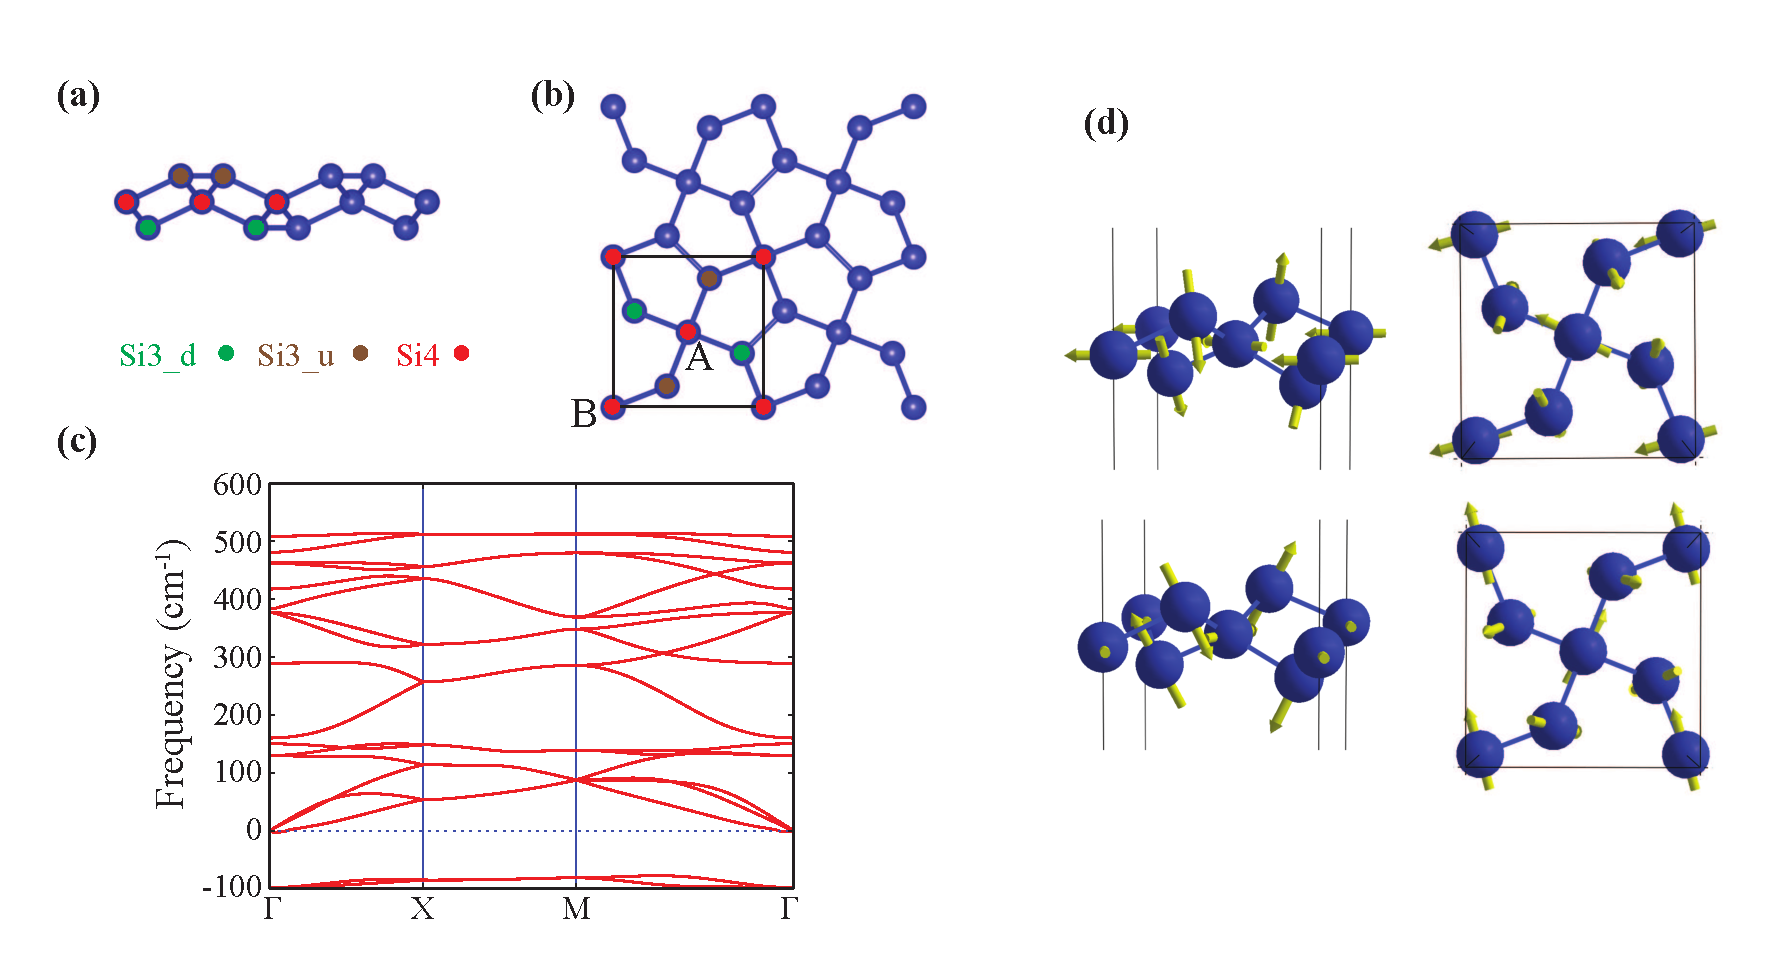
\includegraphics[width=\linewidth]{ps_monolayer.eps}%
\caption{(a) Side view and (b) top view of the atomic structure, (c) phonon spectrum and (d) two vibration modes with imaginary frequency of monolayer penta-silicene. Visualization of vibration modes is done with the V\_Sim package \cite{VSim}. \label{fig:ps_monolayer}}
\end{figure}

The layer group symmetry of monolayer penta-silicene (p-Si) is p$\overline{4}$2$_1$m (58). As shown in \autoref{fig:ps_monolayer}(a) and \autoref{fig:ps_monolayer}(b), the primitive cell contains six silicon atoms, of which two have fourfold coordination (Si4) and four have threefold coordination (Si3). Two of the Si3 atoms reside above the Si4 atoms, denoted as Si3\_u, while the other two are below the Si4 atoms, denoted as Si3\_d. The Si4 atoms are bonded to four Si3 atoms while the Si3 atoms are connected to two Si4 atoms and one neighboring Si3 atom. Note that the two Si4 atoms have equivalent environments which are rotated by approximately 41$^{\circ}$ with respect to each other. Therefore, in analogy to graphene, we can relate these two equivalent Si4 atoms to sublattices which in the following will be referred to as the A and B sublattice.

The dynamical stability of this structure can be studied through its phonon spectrum. As noted before\cite{Ding2015,Li2015b} the phonon spectrum of monolayer p-Si contains imaginary frequencies as shown in \autoref{fig:ps_monolayer}(c), which is a clear signature of its instability. The corresponding atomic vibrations of the two imaginary frequencies at the $\Gamma$ point are shown in \autoref{fig:ps_monolayer}(d). These modes correspond mainly to out-of-plane vibrations of the Si3 atoms with respect to the Si4 atoms. As a consequence, the structure is found to fall apart, indicating that there is no stable form of monolayer p-Si. However, the addition of extra layers could reduce these out of plane vibrations and stabilize the structure. This is the motivation to study few-layer p-Si.


\subsection{Multilayers of pentasilicene structures}\label{fews}

\begin{figure}[htb]
\centering
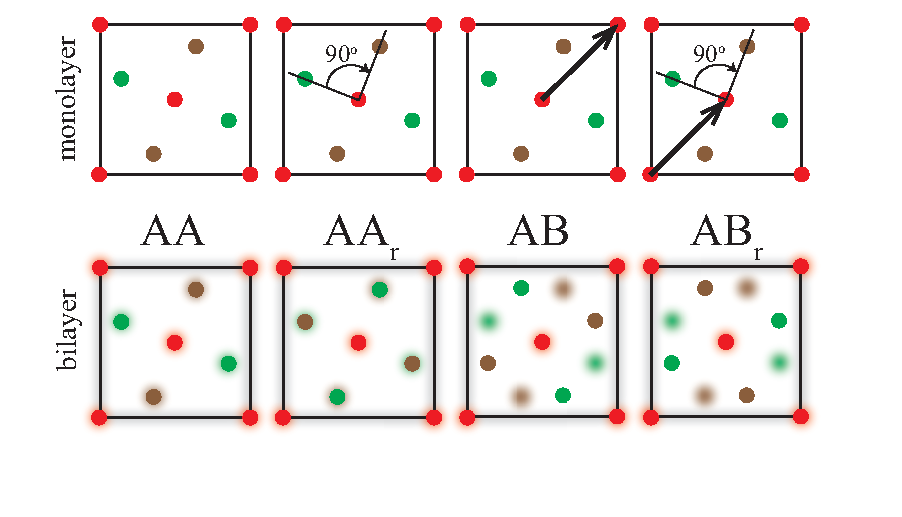
\includegraphics[width=0.8\linewidth]{ps_stackings.eps}%
\caption{ Schematic illustration of the four stacking types for bilayer p-Si. The colors of the symbols correspond to those of the monolayer in \autoref{fig:ps_monolayer}(a) and \autoref{fig:ps_monolayer}(b). The bottom layer in the bilayer is blurred for clarity. The arrow represents translation and the angle represents the rotation of the top layer with respect to the bottom layer. \label{fig:ps_stackings}}
\end{figure}

\begin{table}[htb]
\centering
\caption{The cohesive energy (E$_{\text{coh}}$), the interlayer binding distance (d$_{\text{inter}}$), the interlayer binding energy (E$_{\text{inter}}$), number of interlayer bonds (N$_b$) and energy per bond (E$_{\text{bond}}$) of the four possible stacking types of bilayer p-Si. The interlayer binding energy per unit cell is defined as $E_{\text{inter}}=E_{\text{bi}}-2E_{\text{mono}}$. \label{bilayer_table}}
\begin{tabularx}{\textwidth}{@{\extracolsep{\fill}}X|XXXXX}
\hline\hline
\multirow{2}{*}{structure}  & E$_{\text{coh}}$ & d$_{\text{inter}}$ & E$_{\text{inter}}$& N$_b$ & E$_{\text{bond}}$ \\ 
 & (eV/atom) & (\AA) & (eV) & - & (eV) \\ \hline
AA & -4.129 & 0.795   & -3.502  & 4 & -0.875 \\
~AA$_r$ & -4.113 & 2.379   & -3.318  & 2 & -1.659 \\
AB & -3.968 & 2.174   & -1.574  & 2 & -0.787 \\
~AB$_r$ & -4.147 & 1.893   & -3.725  & 2 & -1.862 \\
~AB$_r^d$ & -4.185 & 1.896   & -4.174  & 2 & -2.087 \\ 
\hline\hline
\end{tabularx}
\end{table}

When considering two layers, different stacking configurations are possible. Here we focus on the so-called AA and AB stacking modes of the aforementioned sublattices (see \autoref{fig:ps_stackings}). The stacking in which both layers have the same in-plane orientation and the Si atoms are put right on top of each other is called AA stacking. AB stacking arises by shifting the A sublattice of one layer to the B sublattice of the other. This nomenclature was also used by \citet{Wang2015} for bilayer penta-graphene. Although penta-silicene has a tertragonal lattice symmetry, the highest proper rotational symmetry order is two. Therefore, there are also two different possible orientations of the upper layer with respect to the lower one:  One in which the two layers have the same orientation and another in which one layer is rotated over 90$^{\circ}$ with respect to the other one. We denote this last orientation with a subscript $r$ to show that it results from a 90$^{\circ}$ rotation, e.g. AA$_r$. Therefore, there are four possible stacking types for bilayer p-Si. Note that AB$_r$ stacking corresponds to the recently proposed bulk T12 phase for group IVA elements\cite{Zhisheng2012}. However, as discussed in more detail below, perfect AB$_r$ stacking is not stable in the case of multilayer penta-silicene.  A considerable distortion of the outer layers is required to stabilize AB$_r$ stacking. The distorted structure, which will be referred to as AB$_r^d$ in the following, is obtained by breaking the symmetry between the two Si3 atoms at each surface side in AB$_r$ multilayers. In this way, one of the two Si3 atoms acquires sp$^2$ hybridization and looses an electron to the other Si3 atom that has sp$^3$ hybridization.

\begin{figure}[htb]
  \centering
  \begin{subfigure}{\linewidth}
    \captionsetup{singlelinecheck=true}
    \includegraphics[width=\linewidth]{ps_AA_structures.eps}%   
    \caption{AA stacked structures \label{fig:ps_AA_structures}}
  \end{subfigure} 
  \begin{subfigure}{\linewidth}
    \captionsetup{singlelinecheck=true}
    \includegraphics[width=\linewidth]{ps_AB_structures.eps}%
    \caption{AB$_r^d$ stacked few-layer and AB$_r$ stacked bulk structures \label{fig:ps_AB_structures}}
  \end{subfigure}
\caption{Atomic structure of the $2\times2$ supercell of few-layer p-Si. The number of atomic layers in the bulk structure is fixed to four for comparison (i.e.\ $2\times2\times4$ and $2\times2\times2$ supercells for AA and AB$_r$ stacked bulk p-Si). (Visualisation using VESTA \cite{vesta}). }
\end{figure}

\begin{landscape}
\begin{table}[htb]
\centering
\begin{threeparttable}[b]
%\adjustbox{max width=\textwidth}{%
\caption{The layer (space) group for few-layer (bulk) systems. The lattice constant ($a$), the interlayer distance (d$_{\text{inter}}$), the nearest-neighbor bond length range (d$_{\text{min/max}}$), the cohesive energy (E$_{\text{coh}}$), and the band gap (PBE) of few-layer and bulk p-Si.}
\label{few-layer-table}
\begin{footnotesize}
\begin{tabular}{ll|lccccccc}
\hline\hline
stacking & structure & layer/space group & $a$ (\AA) & d$_{\text{inter}}$ (\AA) & d$_{\text{min}}$ (\AA) & d$_{\text{max}}$ (\AA) & E$_{\text{coh}}$ (eV/atom) & band gap (eV)   &  \\[3pt]  \hline
-& monolayer & p$\overline{4}$2$_1$m (58) & 5.587  & - & 2.233 & 2.363 & -3.837 &  0.046 (M$\rightarrow \Sigma$) & \\[3pt] \hline
\multirow{4}{*}{AA}
& bilayer    & \multirow{3}{*}{p$\overline{4}$2$_1$m (58)} & 5.907  & 0.795 & 2.363 & 2.468 & -4.129 & metal  &  \\[3pt]
& trilayer   &   &5.887   & 1.085    & 2.330 & 2.606 & -4.108           & metal          &  \\[3pt]
& tetralayer &   & 5.980  & 0.996/1.794\tnote{a}   & 2.368 &	2.478   & -4.150           & metal          &  \\[3pt]
& bulk       & P$\overline{4}$2$_1$m (113)  & 6.234  & 1.769    & 2.398 & 2.463          & -4.204            & metal           &  \\[3pt] \hline
\multirow{3}{*}{AB$_r^d$}                          
& bilayer   & pb2b (30) pm2a (31) & 5.222            & 1.896      &2.303 &	2.403         & -4.185           & 0.119 (M$\rightarrow \Sigma$) &  \\[3pt]
& trilayer  & p1 (1) & 5.222            & 1.989     & 2.298 &	2.413           & -4.291           & 0.247 (M$\rightarrow \Sigma$) &  \\[3pt]
& tetralayer & pb2b (30) pm2a (31) & 5.221            & 1.997       & 2.298	 & 2.413         & -4.345           & 0.232 (M$\rightarrow \Sigma$) &  \\[3pt]
AB$_r$ & bulk      & P4$_2$/ncm(138) & 5.220         & 1.999       & 2.358 &	2.413         & -4.508           & 1.329 (M$\rightarrow \Delta$) & \\ \hline\hline
\end{tabular}
\end{footnotesize}
\begin{tablenotes}
\item [a]The first and the second number indicate the interlayer distance between two monolayers and two bilayers, respectively.
\end{tablenotes}
\end{threeparttable}
\end{table}
\end{landscape}

In \autoref{bilayer_table}, we compare the energies of the different stacking modes. In all cases the Si4 atoms are not involved in interlayer bonding since their possible number of bonds is already saturated.  Except for the AA stacking where all Si3 atoms are bound to Si3 atoms from the other layer, only half of the Si3 atoms are bonded to the other layer in the other cases. In \autoref{bilayer_table}, the size of the interlayer binding energy and the strength per bond are given. The size of the bond energies indicate strong chemical bonding. The  AB$_r^d$ stacking mode clearly forms the most stable structure. For the rest of the section, we will only focus on the most stable AA and AB-type stacking, i.e. AA and AB$_r^d$.

We also investigated the stability of trilayer, tetralayer and bulk p-Si structures by adding extra layers to the stable bilayers mentioned above, their structures are shown in \autoref{fig:ps_AA_structures} and \autoref{fig:ps_AB_structures}. We list their structural and energetic properties in \autoref{few-layer-table}. Extra layers increase the cohesive energy per atom due to a smaller ratio of surface atoms. For AA stacking, adding a 4th layer to a trilayer system results in a double bilayer system with lesser bonding between them. Going to AA bulk, the interlayer interaction appears to be further reduced and the buckled layers become more flat. Adding extra layers to an AB$_r^d$ bilayer results in similar structures in which the Si3 atoms of the surface layers become distorted. For bulk, the undistorted AB$_r$ structure is found in which $\overline{4}$-fold symmetry is restored.



\subsection{Stabilities}\label{stab}

\begin{figure}[htb]
\centering
\includegraphics[width=0.9\linewidth]{ps_phonon_spectrum.eps}%
\caption{Phonon spectra of different-stacked few-layer p-Si. \label{fig:ps_phonon}}
\end{figure}

In this section we investigate the stability of the different multilayer structures discussed above.
Phonon calculations for the AA and AB$_r$ stacking modes reveal that only the AA bilayer is dynamically stable at low temperature. The extra bonds of the Si3 atoms in AA-stacked structures effectively reduce out-of-plane vibrations and stabilize the structure. Although the AA-stacked bulk structure has weaker interlayer bonding, its phonon spectrum contains no imaginary frequencies, indicating its dynamical stability. The AB$_r$-stacked layers, on the other hand, exhibit similar out-of-plane vibrations of the outermost Si atoms as a monolayer. For AB$_r^d$-stacking the distortion of the outermost layer removes the instabilities from the phonon spectrum, so that these structures are also dynamically stable. 

It is also interesting to see whether these structures remain stable at finite temperature. To this end, we performed \textit{ab initio} molecular dynamics calculations at a temperature of 100 K. The evolution of the cohesive energy as a function of simulation time is shown in \autoref{fig:ps_MD}. For comparison, the results for the dynamically unstable monolayer are also shown. The monolayer laterally shrinks and becomes a disordered multilayered system. The AA and AB$_r^d$ bilayer systems, on the other hand, remain stable and retain their crystalline structure.

\begin{figure}[htbp]
\centering
\includegraphics[width=0.7\linewidth]{ps_ab_initio_MD_100K.eps}%
\caption{The cohesive energy of monolayer and AA and AB$_r^d$ stacked bilayer p-Si as a function of time at a temperature of 100 K under NpT-ensemble. \label{fig:ps_MD}}
\end{figure}

As a final stability check, we investigate the mechanical stability of bilayer p-Si which is determined by the elastic constants of the structures. If the elastic constants satisfy the necessary and sufficient Born criteria generalized by \citet{Mouhat2014}, the structures are mechanically stable. AA bilayer p-Si belong to the layer group symmetry of p$\overline{4}$2$_1$m, which belongs to the tetragonal symmetry groups, and the independent elastic constants in 2D are: $C_{11}$= 101.43 N/m, $C_{12}$= 36.36 N/m and $C_{66}$ = 39.53  N/m. In the case of AB$_r^d$ bilayer p-Si, the crystal possesses pb2b or pm2a layer group symmetry which belongs to the orthorhombic crystal systems, and the independent elastic constants are: $C_{11}$=$C_{22}$= 63.83 N/m, $C_{12}$=26.92 N/m and $C_{66}$ = 50.43 N/m.  For mechanical stability, the following criteria must be fulfilled for 2D tetragonal systems:
\begin{equation}
C_{11}>|C_{12}|, C_{66}>0,
\end{equation}
while 2D orthorhombic systems should satisfy:
\begin{equation}
C_{11}>0,C_{11}C_{22}>C_{12}^2, C_{66}>0.
\end{equation}
As one can see, these criteria are satisfied by AA and AB$_r^d$ bilayer p-Si which ensures their mechanical stability. Additionally, in \autoref{mechanical}, we list the  (2D) Young's modulus, shear modulus and Poisson's ratio of bilayer p-Si systems. An interesting aspect of the possion's ratio of AB$_r^d$ is that it is quite high and close to the theoretical limit of 0.5. This means that this 2D material, prefers to change its shape rather than its surface area under strain, similar to the (3D) cases of rubber and water.

\begin{table}[htbp]
\centering
\caption{Mechanical properties of AB$_r^d$ bilayer p-Si}
\label{mechanical}
\begin{tabularx}{0.6\textwidth}{l|XXX}
\hline\hline
Stacking & $E[N/m]$ & $G[N/m]$ & $\nu$ \\ \hline
AA & 88.40 & 39.53 & 0.36 \\ 
AB$_r^d$ & 52.47 & 50.41 & 0.42  \\ \hline\hline
\end{tabularx}
\end{table}

\subsection{Relative phase stability}\label{hexa}

\begin{figure}[htb]
\centering
\includegraphics[width=0.9\linewidth]{ps_h-silicene.eps}%
\caption{Top and side views of the atomic structures of the 2 $\times$ 2 supercell of the three examined hexagonal silicene bilayers. \label{fig:ps_h-Si}}
\end{figure}

\begin{table}[htb]
\centering
\caption{The interlayer distance d$_{\text{inter}}$, the nearest-neighbor bond length range (d$_{\text{min/max}}$) and the cohesive energy per atom E$_{\text{coh}}$ of the most stable hexagonal bilayer silicene and bilayer p-Si. }
\label{h-Si_table}
\begin{tabularx}{0.9\linewidth}{l|XXXX}
\hline\hline
\multirow{2}{*}{structure}  &   d$_{\text{inter}}$ & d$_{\text{min}}$ & d$_{\text{max}}$ & E$_{\text{coh}}$  \\ 
 &   (\AA) & (\AA) & (\AA) &  (eV/atom) \\
 \hline
AA bilayer p-Si  &  0.795  & 2.363  & 2.468  & -4.129 \\
AB$_r^d$ bilayer p-Si  &  1.896  & 2.303  & 2.403  & -4.185 \\
h-Si1            &  2.175  & 2.358  & 2.418  & -4.115 \\
h-Si2            &  1.579  & 2.298  & 2.453  & -4.165 \\
h-Si3            &  1.378  & 2.288  & 2.473  & -4.175 \\ 
\hline\hline
\end{tabularx}
\end{table}

In this section we compare the cohesive energy of bilayer p-Si to the more familiar bilayer hexagonal silicene structures (h-Si).  We examined 3 different stacking types for h-Si bilayers, denoted as h-Si1, h-Si2, and h-Si3. To the best of our knowledge, these are the most stable hexagonal bilayer structures of silicene predicted so far. The h-Si2 structure corresponds to the re-DL-Si structure suggested by \citet{Morishita2011} and the h-Si3 is the hex-OR-2$\times$2 structure that was recently proposed by \citet{Sakai2015}. These structures are constructed from the structure information provided by the authors in the supplementary material of the corresponding papers and re-optimized with our computational procedure. The h-Si1 is a new stable bilayer h-Si structure that we discovered (see ESI\dag~for details). It is composed of two planar, non-buckled, compressed hexagonal silicene planes that are shifted along the crystal plane. This structure is interesting because although its cohesive energy is close to the former two cases, it has a non-buckled nature. To the best of our knowledge, it is the most stable non-buckled bilayer silicene discovered so far. 

The cohesive energies of all the stable bilayer Si systems are given in \autoref{h-Si_table}. It is seen that the AB$_r^d$ bilayer p-Si system has the lowest energy, about 10 meV/atom less than the most stable hexagonal silicene bilayer h-Si3.  This means that the AB$_r^d$ p-Si structure is the most stable bilayer silicon structure predicted so far, which is a very surprising result. The AA-stacked p-Si has slightly higher energy than h-Si2 and h-Si3.

\subsection{Electronic properties}\label{elec}

\begin{figure}[htbp]
\centering
\includegraphics[width=0.8\linewidth]{ps_AA_bands.eps}%
\caption{Electronic band structure of AA stacked few-layer and bulk p-Si, and a schematic of the first Brillouin zone. \label{fig:AA_bands}}
\end{figure}

\begin{figure}[htbp]
\centering
\includegraphics[width=0.8\linewidth]{ps_AB_bands.eps}% 
\caption{Electronic band structures of AB$_r^d$ stacked few-layer and AB$_r$ stacked bulk p-Si. The results for the monolayer are shown for comparison.\label{fig:AB_bands}}
\end{figure} 

\begin{figure}[htbp]
\centering
\includegraphics[width=0.7\linewidth]{ps_charge_density.eps}%
\caption{The charge distribution of CBM and VBM in AB$_r^d$ stacked few-layer and AB$_r$ stacked bulk p-Si. The results for the monolayer are shown for comparison.\label{fig:charge_density}}
\end{figure}

In the last part of this work, we investigate the electronic properties of few-layer and bulk p-Si. These electronic properties are mainly determined by the electronic spectrum. In \autoref{fig:AA_bands} and \autoref{fig:AB_bands}, the electronic band structure of respectively AA and AB$_r^d$ p-Si multilayers and their bulk counterpart is shown. The band structure of the unstable monolayer is also calculated for comparison. Monolayer p-Si is an indirect semiconductor with a band gap of 0.046 eV (PBE). The band-edge states are mainly composed of $p_z$ orbitals of Si3 atoms. In contrast to this, all AA-stacked multilayers are metallic. In the case of the AB$_r^d$ structure, the semiconducting properties of monolayer p-Si are preserved, but the band gap changes somewhat with the number of layers. This can be understood from the position of the electron and hole states which correspond to the CBM and the VBM, respectively. As seen in \autoref{fig:AB_bands}, the VBM and CBM states are always localized on the outermost layers. In other words, the electronic properties are mainly determined by the surface region which is nearly independent of the slab thickness. For AB$_r$-stacked bulk p-Si, there is no surface and the VBM and CBM correspond to bulk states. This explains the much larger band gap (1.33 eV) in the bulk case. 


\subsection{Summary}

In this work, we proposed several stable structures for few-layer pentasilicene. The stability of these structures was confirmed via their phonon spectrum, finite-temperature molecular dynamics, and their mechanical properties. The type of stacking mode, AA or AB, of few-layer pentasilicene has a crucial influence on the electronic properties: AA-stacked systems are metallic, while AB$_r^d$ stacked ones are semiconducting . Surprisingly, the AB$_r^d$ stacked bilayer pentasilicene has lower energy than the most stable bilayer hexagonal silicene structures, which makes it the most stable predicted form of bilayer silicon.  

\section[Mechanical strain: Carrier mobility enhancement in TiS$_3$ monolayer with strain]{Mechanical strain: Carrier mobility enhancement in TiS$_3$ monolayer with strain \footcite[This work is published in:][]{Aierken2016.mobility} \label{mob_Tis3}}

\subsection{Introduction}

Recently, a number of 2D crystal materials  beyond graphene \citep{Novoselov666,Novoselov26072005,Geim2007} have been synthesized or have been theoretically predicted to be stable. For example, TMDs \cite{RadisavljevicB2011,Zeng2011,Ataca2012,Liu2015, tongay-res2, PhysRevB.89.155433}, phosphorene family \cite{p1,Han2014,Adam2015,Guan2014,deniz1,deniz3}, transition metal carbides/carbonitrides (Mxenes)\cite{ADMA:ADMA201304138}, and penta-graphene \cite{Zhang2015} have attracted a growing research interest.  Many of these materials have distinct properties with respect to their bulk counterpart, ranging from the nature of the band gap\cite{Mak2010} to the size of the thermal conductivity \cite{Alexander2008}.  For future electronic device applications, it is the high mobility and band gap of these materials, which has drawn significant attention of the researchers. Although graphene is a fascinating material due to e.g. its ultra high mobility, it has however one significant disadvantage, i.e. it lacks a band gap, and thus is unsuitable for digital electronic applications. This drawback has triggered  extensive efforts to search for new materials  having a finite band gap and high mobility. Recently synthesized phosphorene and monolayer TiS$_3$\cite{ADOM:ADOM201400043,ADMA:ADMA201405632} are examples of such promising materials for high-performance applications. On the other hand, the modification of physical and chemical properties through various methods, e.g. chemical functionalization, heterostructure and mechanical strain, could pave a path for the exploration of the hidden features which do not manifest themselves at the pristine structure. 

Enhancement of the mobility under strain has been reported and measured before for silicon layers on Si$_x$Ge$_{1-x}$ substrates \cite{Vogelsang1993,Welser1994}, according to which a mobility enhancement up to about 76 \% at room temperature was achieved. Recently, first-principles calculations have been frequently used to determine the intrinsic mobility of 2D materials.\cite{Kaasbjerg2012,Zhang2014,Yongqing2014}. There are also several works that investigated the mobility of monolayer materials under strain\cite{fei,Henry2015,Sheng2015}, including strain-controlled anisotropic of mobility in phosphorene \cite{fei}, vertical compression of phosphorene bilayer leads to two orders of magnitude increment of mobility\cite{Henry2015}, strain-enhanced mobility of MoS$_2$ up to a factor of 10 \cite{Sheng2015}. In the last two cases, enhancement of mobility contribute from decrease of DPC which consist with our situation that will be discussed in our results. Inspired by significant improvements of the transport properties of 2D materials by the help of appropriate strain type and size, we investigate the strain dependence of  carrier mobility of TiS$_3$ monolayer under mechanical strain at 300 K. We find that more than an order of magnitude enhancement of the electron mobility can be achieved by the tensile strain. Furthermore the hole mobility also has moderate enhancement.


\subsection{Computational details}

\begin{footnotesize}
\begin{description}
\item[Simulation program:] VASP and Phonopy
\item[Energy cut-off:] 700 eV
\item[Pseudopotentials:] PBE-GGA(PAW)
\item[k points (Monkhorst-Pack):] 25$\times$25$\times$1 for insulating and metallic systems, respectively 
\item[Vacuum:] 20~\AA
\item[Energy and force convergence criterion:] 10$^{-8}$ eV and 10$^{-7}$ eV/\AA, respectively
\item[phonon calculation:] finite displacement method
\item[Supercell for phonon calculation:] $2\times3\times1$
\end{description}
\end{footnotesize}


Band gap is underestimated due to well-known semilocal functional band gap problem. However, for the position shifts of the valence and conduction band edges with an applied tensile strain, the semilocal functional can provide consistent results and trends when compared to hybrid functionals and has  been successfully used in  previous studies for the determination of the mobility in 2D material \cite{Meng-Qiu2009,Yongqing2014,fei}. 

To determine the mobility of electron and  hole, we use the deformation potential theory together with the effective mass approximation \cite{Bardeen1950}, which has been previously applied to several 2D systems\cite{Xi2012,Qiao2014a,Dai2015,Kang2015}.
The mobility, $\mu$, of a 2D system is given by: 
\begin{equation} \label{equ}
\mu=\frac{2e\hbar^3C}{3k_BT|m^*|^2E_d^2}.
\end{equation}
where $e$ is the electron charge and $\hbar$ is the reduced planck constant. $C$ is the elastic modulus along the transport direction. It is defined as $C=(\partial^2E_{total}/\partial\varepsilon^2)/S_0$, where $E_{total}$ is the calculated total energy of TiS$_3$, $\varepsilon$ is the strain applied along the transport direction and $S_0$ is the equilibrium 2D area of the unit cell. $k_B$ is the Boltzmann constant. T is the temperature, which is equal to 300 K throughout the section unless stated otherwise. $m^*$ is the effective mass of the carrier along the transport direction calculated from $1/m^*_{e(h)}=\partial^2E_{c(v)}(k)/\partial k^2\hbar^2$, where $E_{c(v)}(k)$ is the energy dispersion near the CBM (VBM). $E_d$ is the DPC along the transport direction. It is defined as $E_d^{e(h)}=\Delta E_{CBM(VBM)}/(\delta l/l)$, where $\Delta E_{CBM(VBM)}$ is the energy shift of the band edges with respect to the vacuum level under a small dilation $\delta l$ of the lattice constant $l$. We fix $\delta l/l$ to 0.005 that is inspired from previous calculations \cite{Dai2015}. In this theory,  the dominant scattering process is the longitudinal acoustic phonon scattering (AS). However, for a polar material, scattering on  optical phonon modes and other scattering sources should be taken into account at high temperatures\cite{Kaasbjerg2012}. Nevertheless, in this work, we will focus solely to the effect of AS to mobility and its dependence on the strain for the following reasons: 1) The dominant role of AS is not suppressed in polar materials, so it is still an important part that determines the mobility, 2) To separately study different mobility-controlled mechanism, specially their strain dependence, and 3) Computationally less expensive. 


\subsection{Unstrained system}

\begin{figure}[htb]
\centering
\includegraphics[width=0.6\linewidth]{Mob_str.eps}
\caption{(a) Top and (b) tilted views of a 2$\times$2 supercell of monolayer TiS$_3$.  Two crystallographic directions (where the strain is applied or the mobility is calculated) are shown with red and green arrows. \label{tis3_structure} }
\end{figure}

The atomic structure of TiS$_3$ monolayer is shown in \autoref{tis3_structure}. The unit cell has a monoclinic crystal structure. The calculated lattice constants  are \textit{a} =  5.03 ~{\AA} and \textit{b} = 3.41~{\AA}, in good agreement with previous calculations \cite{Kang2015,Jin2015} and close to the experimental values for the bulk structure ($a$=4.958, $b$=3.401)\cite{Furuseth1975}. The monolayer is composed of connecting quasi-one-dimensional chains of TiS$_3$ triangular prisms extending along the \textit{b} direction, as shown in \autoref{tis3_structure}. One can spot a significant structural anisotropy in the system along the chain direction (green vector) and  the perpendicular direction (red vector). Therefore, we can make a clear distinction when discussing between these two directions throughout the section.

\begin{figure}[htb]
\centering
\includegraphics[width=0.8\linewidth]{Mob_projected_bands.eps}
\caption{(a) The site and orbital-projected band structure (calculated using PBE functional) of the unstrained TiS$_3$ monolayer.  Decomposed charge density of CMB (b) and  VBM (c) at the $\Gamma$ point are presented. \label{band} }
\end{figure}

As is shown in \autoref{band}, monolayer TiS$_3$ is a direct band gap semiconductor having a band gap of 0.29 eV (1.06 eV \cite{Dai2015}) calculated with PBE (HSE06) functional at the $\Gamma$-point.  The CBM has the largest contribution from d$_{x^2-y^2}$ and d$_{z^2}$ orbitals of the Ti atoms, while the VBM is mostly dominated by the p$_x$ orbital of the S atoms and  the $d_{xz}$ orbitals of the Ti atoms. The $x$ and $y$ directions coincide with the \textit{a} and \textit{b} directions, respectively. The $z$ direction is taken perpendicular to the $xy$ plane. Later, we will discuss in detail how these states change their energies when they are exposed to the mechanical strain.

To gain deep insight about the binding nature in the TiS$_3$ monolayer, we calculate the Bader charges\cite{Bader1,Bader2,Bader3,Bader4}. According to the Bader analysis, each Ti atom donates 1.61 $e^-$ to eight S atoms surrounding it. Each of the surface S atoms, labelled as S1 in \autoref{band}, binds only with two Ti atoms and gain 0.34 $e^-$ net charge. Two of these S1 atoms form a covalent bond between them. While each of the S atom between two Ti layers, S2 in \autoref{band}, binds with four neighboring Ti atoms, and have 0.81 $e^-$ net charge accumulated on it.  The electronegativity differences between S (2.58) and Ti (1.54) is calculated as 1.04, which belongs to the polar covalent bond class \cite{David2015}.  This value is large as compared to that of MoS$_2$ where Molybdenum (2.16) and S (2.58), which is 0.41 and is considered as covalent bond type.

\begin{table}[ht]
\caption{The electron (hole) effective mass ($m^*$), the elastic modulus ($C$), the DPC ($E_d$), and the electron (hole) mobility ($\mu$) of phosphorene and monolayer TiS$_3$.}
\centering
\begin{footnotesize}
\begin{tabularx}{\textwidth}{l|lXXXXXX}
\hline\hline
Material & Carrier type & Direction & $m^*$($m_e$) & $C$(N/m) & $E_d$(eV) &  $\mu$(10$^3$ cm$^2$V$^{-1}$s$^{-1}$)\\ \hline
\multirow{2}{*}{Phosphorene} & electron & armchair & 0.20 & 24.30 & 0.65 &  1.93 \\
& hole & zigzag & 6.89 & 103.14 & 0.11 & 25.36 \\ \hline
\multirow{4}{*}{TiS$_3$ monolayer} & \multirow{2}{*}{electron} & \textit{a} & 1.52 & 82.68 & 0.53 & 1.82 \\
&   & \textit{b} & 0.40 & 133.76 & 0.84 & 17.08 \\ 
& \multirow{2}{*}{hole} & \textit{a} & 0.30 & 82.68 & 2.53 & 2.00 \\ 
&   & \textit{b} & 0.99 & 133.76 & 4.10 & 0.11 \\ \hline\hline

\end{tabularx}
\label{unstrain}
\end{footnotesize}
\end{table}

Before  applying strain to our system, we summarize  the mobility and related parameters for the unstrained TiS$_3$ in \autoref{unstrain}, which are in agreement with previous calculations \cite{Dai2015}. Similar data for phosphorene are presented for comparison. The results for phosphorene are recalculated with the same computational parameters as TiS$_3$. The mobility of the electron in TiS$_3$ monolayer has an impressive level, which is an order of magnitude larger than that in phosphorene. However, resulting from very small DPC, hole mobility in phosphorene is an order of magnitude larger than that in TiS$_3$.  Moreover, the anisotropy of the effective mass along different crystallographic directions is much more significant for phosphorene as compared to that in TiS$_3$. Phosphorene overall is softer than TiS$_3$ as far as the elastic modulus is concerned.

\subsection{Dynamical stability under  mechanical strain}

\begin{figure}[htb]
\centering
\includegraphics[width=0.6\linewidth]{Mob_stiffness.eps}
\caption{Calculated elastic modulus along the \textit{a} and \textit{b} directions under mechanical strain. \label{stiffness}}	
\end{figure}

Applying mechanical strain may have important effects on the stability of a structure. Therefore, it is crucial to know if  strain applied to the system does not induce any structural instability. To this purpose, we calculate the elastic modulus and phonon spectrum for the TiS$_3$ monolayer under various strain values in order to confirm its dynamical stability.  \autoref{stiffness} shows the elastic modulus along the \textit{a}  and \textit{b}  directions as a function of applied strain. These values correspond to the elastic constants, i.e.  C$_{11}$ and C$_{22}$.  Here, C$_{11}$ (C$_{22}$) reflects the mechanical response of the TiS$_3$ monolayer to a strain applied along the \textit{a} (\textit{b}) direction.  The calculated value of C$_{11}$ (C$_{22}$) for the unstrained TiS$_3$ is 133.76 (82.68) N/m, in good agreement with previous calculations \cite{Dai2015,kang2015m}. Note that the calculated elastic constants are all positive and they fulfill the mechanical stability criteria, i.e. C$_{11}$ and C$_{22}$ $>$ 0. These results clearly imply that monolayer TiS$_3$ is less stiff than graphene and single layer h-BN, however, it is mechanically superior as compared to MoS$_2$ and phosphorene\cite{deniz2}. Furthermore, C$_{22}$ is always larger than C$_{11}$, meaning that the \textit{a} direction is stiffer than the \textit{b} direction. 

In order to gain further insight into the stability of TiS$_3$ monolayer, we calculate the phonon dispersion under different types of strain. As shown in \autoref{phn},  uniaxial strain applied along the \textit{a} and \textit{b} direction induce dynamical instability in the system at strain values of 6\% and 8\%, respectively.  Note that the highest optical mode reaches up to ~550 cm$^{-1}$ and does not vary with strain. Consistence with our results of the elastic constants, the optical phonon modes are more sensitive to strain applied along the \textit{b} direction, see \autoref{phn}. Except for the topmost mode,  phonon branches move downward with strain applied along the \textit{b} direction.  We observe an average downward shift of 25 cm$^{-1}$ at 8\%, which should be easily detected by Raman spectroscopy.  The observed instability at large strain values is due to the presence of imaginary vibrational frequencies, suggesting a structural phase transition. The dynamical stable range of black phosphorus is 15\% which is much larger than that of TiS$_3$\cite{0953-8984-27-17-175006}.  Due to its puckered structure, the former is able to sustain large mechanical deformations.  The biaxial case is the combination of two uniaxial strains applied along the \textit{a} and \textit{b} directions, and the stable range is determined by the lowest strain value, i.e. 6\% applied along the \textit{a} direction. 

\begin{landscape}
\begin{figure}[htb]
\centering
\includegraphics[width=\linewidth]{Mob_phn.eps}
\caption{Calculated phonon spectrum of (a) pristine monolayer TiS$_3$ and that under strain (b-g). }
\label{phn}
\end{figure}
\end{landscape}

\subsection{Bond lengths and band gap under mechanical strain}
The foremost consequence of the mechanical strain is the change of the structure parameters in the unit cell. Strain is applied by manually changing the lattice constant along the desired direction. After that, the cell parameters are kept fixed whereas the internal atomic positions are allowed to fully relax. Therefore, the latter can be considered as the response of the material to the external strain, which would carry important information about the consequential effects. The variation of the bond length provides information about how the local environment of atoms in the unit cell changes with strain. Considering this, we plot the bond lengths with respect to the different types of strain in \autoref{bonds}. 

\begin{figure}[htb]
\centering
\includegraphics[width=0.8\linewidth]{Mob_bonds.eps}
\caption{Variation of bond lengths with strain. Color of the curves matches with the color of the bonds in the structure depicted in the inset.\label{bonds}}
\end{figure}


\begin{figure}[htb]
\centering
\includegraphics[width=0.6\linewidth]{Mob_bandedges.eps}
\caption{Variation of the band edges with respect to vacuum with strain. \label{bandedges}}
\end{figure}

In the following discussion, we correlate the variation of the CBM and VBM, as shown in \autoref{bandedges}, with the change of bond length by investigating their bonding character. Let us first focus on strain applied along the \textit{a} direction. The most significant change occurs for the Ti-S bond between two neighboring prisms. As the strain increases, the local environment inside the prism hardly changes, whereas the bond lengths of Ti-S bonds between prisms. On the other hand, it can be seen from the decomposed charge density of the VBM at the $\Gamma$ point for the unstrained TiS$_3$ (see \autoref{band}(c)) that the Ti-S distance between two prisms is controlled by the Ti-S bonding state at the VBM. Therefore, we would expect that the energy of this state increases (i.e. its binding energy decreases) with tensile strain, which can be seen in \autoref{bandedges}. For strain applied along the \textit{b} direction, one can note from \autoref{band}(c) that the VBM charge distribution along the \textit{b} direction has a node between two prisms. Given the fact that atoms sit close to each other, this is an  anti-bonding state. Therefore, we would expect that its energy decreases (i.e. its binding energy increases by depopulating the anti-bonding state) when strain along the \textit{b} direction increases. This is true when we see the trend of the VBM with the strain applied along the \textit{b} direction in \autoref{bandedges}. The CBM mostly gives a nonbonding state regardless of the direction, see \autoref{band}(b). This results in a much slower variation of the energy of  the CBM under tensile strain, yet only an overall small change is observed. 

\autoref{bandedges} also provides information about the variation of the band gap under strain, which agrees well with previous calculations \cite{Biele2015,Li2015}. While the band gap decreases under strain applied along the \textit{a} direction, it increases with strain applied  along the \textit{b} direction. The band gap increase in the latter case was experimentally confirmed \cite{Biele2015}.  By the help of  strain engineering, it is possible to tune the optical gap from far infrared to near infrared. The nature of the band gap remains direct within the considered tensile strain range where TiS$_3$ is dynamically stable. We find that  biaxial strain is a superposition of the above two situations as can be seen from \autoref{bandedges}. 

\subsection{Effective mass, DPC and mobility under  mechanical strain}

\begin{figure}[htb]
\centering
\includegraphics[width=0.6\linewidth]{Mob_emass.eps}
\caption{Variation of the effective mass of electron and hole along the \textit{a} and \textit{b} directions at the $\Gamma$-point with strain. \label{emass}}	
\end{figure} 

Using the computational setup described above, we estimate the acoustic-phonon-limited mobility of monolayer TiS$_3$ under  strain via \autoref{equ}. According to this equation, at a particular temperature (e.g. 300 K),  three different physical parameters, namely elastic modulus $C$, carrier effective mass $m^*$ and DPC or $E_d$,  are subjected to a change under strain. Previously, we already discussed the variation of the elastic modulus with strain, which is shown in \autoref{stiffness}. Now we discuss how the effective mass and DPC change under strain. \autoref{emass} shows the effective mass of both hole and electron for different directions and strain values. All curves change monotonically. There is no abrupt change of the slope of the curves since there is no band crossing in the considered strain range, and one would expect a smooth variation for the band edges with strain. The electron mass along the \textit{a} direction increases regardless of the direction of applied strain, and the magnitude of this change is the largest among both carrier effective masses along the other directions. Because of this, the degree of anisotropy in the effective mass increases as TiS$_3$ is subjected to strain. As for the hole effective mass, the difference along the \textit{a} and \textit{b} directions increases for strain applied along the \textit{a} direction whereas this difference decreases for strain applied along the \textit{b} direction. Such anisotropy can be utilized to modify the electronic and thermoelectric properties of TiS$_3$.  

\begin{figure}[htb]
\centering
\includegraphics[width=0.6\linewidth]{Mob_dePotential.eps}
\caption{Variation of the (a) DPC ($E_d$) with strain. \label{dePotential}}
\end{figure}

Our calculations unveil that one of the most important  factors  that determines the mobility is the DPC.  In order to evaluate DPC, we need to apply a small dilation  along the direction where DPC is calculated. The ratio of the CBM (VBM) shift  to the amount of this dilation gives DPC for electron (hole), see \autoref{dePotential}. Mathematically, as shown in \autoref{equ}, it is the square of a small number in the denominator. Thus the variation of DPC determines the whole ratio in \autoref{equ} hence the mobility, unless other quantities change dramatically, which is not the case as we have discussed. For example, in the work of \citet{fei}, they reported the direction of the highest mobility change by 90$^{\circ}$, which was a result of the change in the smallest effective mass in a particular direction. In our case, we  observe no band crossing  and the variation of the  effective mass with strain is rather small for the highest mobility directions, see \autoref{emass}.   

\begin{figure}[htb]
\centering
\includegraphics[width=0.6\linewidth]{Mob_mobility.eps}
\caption{Variation of the mobility ($\mu$) with strain.\label{mobility}}
\end{figure}

Next, we explore the mobility variation under strain, see \autoref{mobility}. For uniaxial strain along the \textit{a} direction, the two most apparent changes are the moderate enhancement of the hole mobility along the \textit{b} direction, from 2.00$\times10^3$ to 7.08$\times10^3$ cm$^2$V$^{-1}$s$^{-1}$ and the drop of the electron mobility along the same direction, from 1.82$\times10^3$ to 0.25$\times10^3$ cm$^2$V$^{-1}$s$^{-1}$. Although the electron mobility along the \textit{a} direction for strainless TiS$_3$ is close to the hole mobility along the same direction, an order of magnitude difference can be realized by the help of tensile strain. Therefore,  uniaxial strain applied along the \textit{a} direction would be helpful to select carrier type based on their different transport properties.  For uniaxial strain along the \textit{b} direction, we find a dramatic enhancement of the electron mobility along the \textit{a} direction, from 1.71$\times10^4$  to 5.53 $\times10^5$ cm$^2$V$^{-1}$s$^{-1}$ at 300 K. This corresponds to a mobility enhancement from 5.13$\times10^4$ to 1.66$\times10^6$ cm$^2$V$^{-1}$s$^{-1}$ at 100 K. The subsequent drop at 7 \% can be ascribed to being close to the edge of the dynamical stable region. Furthermore, the electron mobility in the other direction (i.e. \textit{b}) has a moderate enhancement at strain value of 6 \% as well. The electron mobility along the \textit{b} direction has a considerable increase when tensile strain is applied along the \textit{b} direction. The hole mobility generally tends to decrease on both directions.  As stated before, the biaxial case is an effective combination of two uniaxial strains applied along the \textit{a} and \textit{b} directions. The electron mobility along the \textit{a} direction reaches up to  3.68 $\times10^5$ cm$^2$V$^{-1}$s$^{-1}$ at 5\% biaxial strain. 

Lastly, we discuss the effect of the optical phonon scattering on the mobility.  Using a Drude-like expression, $\mu$ can be expressed as  $\sim$ $q\langle\tau\rangle/m^*$, where $\langle\tau\rangle$ is the average scattering time, and in the Matthiessen's Rule, it is given as sum of all scattering process, i.e.  $1/\tau$=$1/\tau_{ph}$+ $1/\tau_{el}$+$1/\tau_{imp}$+ $\cdots$. Here, $\tau_{ph}$, $\tau_{el}$ and $\tau_{imp}$ are the scattering times related to electron-phonon, electron-electron and electron-impurity scattering, respectively.  In a rough estimate (i.e using Einstein's model), $\tau_{ph}$ for the longitudinal optical phonon scattering is inversely proportional  to the frequency of the optical modes. According to our calculations, the frequency of the phonon modes is subject to a redshift under strain. This means that the contribution of the optical phonon scattering reduces with increasing tensile strain.  As a result, we can claim that our trends are persistent against the contribution of the different scattering processes. 

\subsection{Summary}

In this work, we have demonstrated that, by the help of tensile strain, it is possible to enhance the carrier mobility of the TiS$_3$ monolayer more than an order of magnitude at 300 K and two orders of magnitude at 100 K. Phonon dispersion calculations revealed that TiS$_3$ becomes dynamically unstable for an uniaxial tensile strain larger than 6\% (8\%) applied along the \textit{a} (\textit{b}) direction. The degree of effective mass anisotropy can be controlled with uniaxial strain. The deterministic role of the DPC on the mobility in this material is confirmed. The variation of the CBM and VBM with strain was explained through the bonding character within the TiS$_3$ monolayer.  Here, we also showed that strain engineering appears as a quite exciting way to tune the electrical conductivity of TiS$_3$, which is potentially useful for device applications including flexible electronics.

\section[Heterostructures: Electrical transport in 1T/2H/1T MoS2 lateral heterostructure]{Heterostructures: Electrical transport in 1T/2H/1T MoS2 lateral heterostructure \footcite[This work is submitted as:][]{Aierken2017.transport} \label{trans_mx2}}

Another way to explore the property land of materials is to combine different composites to form heterostructurse\cite{Geim_Grigorieva_2013,Liu2016b,Pomerantseva2017}. They can be composites made by materials with complementary characters and perform better than each of the material individually, or materials those give new phenomenon and promising properties only when act together.  Given the obvious structure anisotropic in 2D materials, there are two types of heterostructures: vertical or lateral, see for example \autoref{fig:ver-lat-stru}. The vertical heterostructures composed of stacks of different 2D materials. They are held together via what holds graphite layers together: vdWs force. Thus, this type of construction is referred as vdWs heterostructures.  On the other hand, lateral heterostructure\cite{Jena2014,Chhowalla2015} is made by joining the edges of different 2D materials and the connection is mostly made through strong bonding, e.g. covalent or ionic. For this case, all the new properties results from the interface. In this section, I will present one for each type of the heterostructure and explore one properties. Comparisons will be made to illustrate the advantage of choosing these materials over the homo-structure. 

\begin{figure}[htbp]
\centering
\includegraphics[width=0.9\textwidth]{ver-lat-stru.png}
\caption{ (a) and (d) vertical and (c) and (d) lateral WS$_2$/MoS$_2$ heterostructures. \label{fig:ver-lat-stru} Image adapted from: \cite{Gong_Lin2014}}
\end{figure}

\subsection{Introduction}
Heterostructures are the essential components of a wide range of solid-state devices, such as transistors, solar cells, and sensors\cite{singh1993,agostini2011}. They are  fabricated by combining different type of materials, e.g. metal, semiconductor, and insulator. Therefore, the physical properties of the combined system are enhanced or become more controllable as compared to that of each material individually. These tailored properties are strongly related to the interface of two different materials where all interesting and new phenomenon occur. However, along with the emergence of nanostructured materials, dimensionality has become another major factor affecting the physical properties of materials and devices along with the interface. Thus, solid-state device fabrication with heterostructures based on low dimensional nanomaterials has attracted significant attention and a new research area in material design has been initiated where researchers are expecting unprecedented results, phenomenon and physics\cite{Gan2013,Wu2015c,DiBartolomeo2016}. Indeed, several advantages of 2D phase engineering over the 3D counterpart has already been demonstrated.\cite{Duerloo2015}

In low dimensional heterostructure device architectures, there are usually two types of interfaces connecting different materials: top contact (vertical) and edge contact (lateral)\cite{Allain2015}. In top contacts, an overlapping portion of two materials are glued together mainly via interlayer vdWs interaction, while in edge contacts one dimensional edges of two materials are contacted with covalent bonds without overlapping. The vdWs interaction in top contact introduces a potential gap between the two layers which electrons have to tunnel through, and resulting in higher resistance due to the reduced carrier transmission probability. Naturally, this resistance is much lower in edge contacts owing to the formation of covalent bonds that provides a path for carriers to travel across the interfaces\cite{Matsuda2010,Kang2014}. Recently, Eda \textit{et al.}  has discovered the coexistence of multi-phase MoS$_2$ that is a promising material for heterostructure device fabrication due to their natural metal-semiconductor-metal structure with clear edge contacts\cite{Eda2012}. Considering the distinct electronic nature of these phases, physical properties of these heterostructures\cite{Kappera2014,Fan2015} can be tuned by phase engineering and novel solid-state device architectures can be realized for several different future applications.

The same research group has synthesized 2D semiconducting heterostructure devices\cite{Huang2014,Zhang2015} by using metal contacts. As a result of their experimental analysis, they have particularly pointed out the vital importance of the geometry and electronic nature consistency between the metal contact and the heterostructure on the device performance\cite{Bai2013,Eda2012}. Considering this fact, Kappera \textit{et al.}\cite{Kappera2014} have locally induced 1T metallic phase of MoS$_2$ in the 1H semiconducting phase of it, and they measured that the edge resistance was lower than that of metal contacts by more than a factor of two. Subsequently, 1T$\mid$1H lateral heterostructure has been drawn peculiar attention as a promising contact structure having a higher carrier injection rate. Different arrangements of the interfaces between 1T and 1H phases was investigated through theoretical calculations\cite{Hu2015,Sivaraman2016} and the structure formed by the connection of armchair edges of 1T and 1H phases has been determined as an energetically more favorable configuration. However, in these calculations, the more stable metallic structure (1T$_d$), which arises with small distortion of 1T phase, was considered.

The present work aims to investigate the electronic transport properties of MoS$_2$ multi-phase lateral junctions when the more stable metallic phase of MoS$_2$ ( i.e. 1T$_d$) acts as the contact, which is compared with the 1T phase. Further to this, this work mainly focuses on the effect of doping on the electrical transport properties. In the results section, we first construct three junction models and calculate their transmission without external bias . Then we calculate the electronic properties for different level of doping.



\subsection{Computational details}


\begin{footnotesize}
\begin{description}
\item[Simulation program:] VASP
\item[Energy cut-off:] 500 eV
\item[Pseudopotentials:] PBE-GGA(PAW)
\item[k points (Monkhorst-Pack):] 25$\times$25$\times$1 for 2D systems and 9$\times$1$\times$1 for lateral heterostructures
\item[Vacuum:] 15~\AA
\item[Energy and force convergence criterion:] 10$^{-5}$ eV and 10$^{-2}$ eV/\AA, respectively
\end{description}
\end{footnotesize}


\paragraph{Transmission spectrum calculation} Electronic transport across the 1T$_d$/1T-MoS$_2$ $\mid$1H-MoS$_2$ interfaces is calculated using the self-consistent NEGF technique as implemented in TranSIESTA\cite{transiesta} which is interfaced with the SIESTA code.\cite{siesta} Double-zeta (plus polarization) numerical orbital basis sets are used for all atoms. We employed norm-conserving pseudo-potentials\cite{tm}, the GGA/PBE functional, and an energy cutoff for the real-space mesh of 250 Ry.  In order to get accurate transmission spectra, the 2D Brillouin zone normal to the transport direction is sampled by meshes composed of  100 $k$-points in the periodic direction. While the SIESTA code uses a localized basis set and norm-conserving pseudopotentials, the calculated lattice parameters for different phases of MoS$_2$ agree well with those obtained from the VASP code. 


\subsection{Structures}

\begin{figure}[htb]
\centering
\includegraphics[width=0.8\linewidth]{structure.eps}%
\caption{\label{structure-1t}  Device models where 1H phase of MoS$_2$ is sandwiched between metallic MoS$_2$ electrodes. In (a) the $\alpha$-device, (b) the $\beta$-device, and (c)
the $\gamma$-device. For the $\alpha$ and $\beta$ devices, 
the interfaces between metallic and semiconducting MoS$_2$ have an armchair termination while a zigzag termination in the $\gamma$-device. }
\end{figure}

The use of metallic TMDCs as metal electrodes are expected to offer a breakthrough in the semiconductor industry as they have negligible heat dissipation and therefore are energy efficient. Among metallic TMDCs, metallic phases of MoS$_2$ (1T- and 1T$_d$-MoS$_2$) have attracted a growing interest due to its smooth interface with  the semiconductor phase of MoS$_2$ (1H-MoS$_2$). 
However, 1H phase is thermodynamically more stable than both 1T and 1T$_d$ phases. Therefore, the stabilization of 1T and 1T$_d$  over 1H phase becomes an essential requirement for the successful experimental realization of device configurable structures such as 1T/T$_d$-MoS$_{2}\mid$1H-MoS$_2$. On the other hand, 1T MoS$_2$ is the meta-stable and undergoes a Peierls transition to a low-energy state 1T$_d$ (or distorted 1T) and thus, metal contacts with the 1T$_d$ structure are more stable than the one with the 1T phase. However, the MoS$_2$ 1T$_d$ phase retransforms to the 1H phase at room temperature. 
As far as the relative stability is considered, choosing 1T$_d$ as metal contact further stabilized the junction.
Therefore, understanding the effect of different physical mechanisms on the stability of multiple phases (H, T, T$_d$) of this material is of vital importance to develop a proper control on phase transitions. To this end we mainly focus on the effect of doping (either charge or atom) on the stability, electronic and transport properties of 1T/T$_d$-MoS$_2\mid$1H-MoS$_2$ interfaces.  For the 1T and 1H hexagonal unit cells, the optimized in-plane lattice constant is obtained as 3.18 {\AA} .  On the other hand, the optimized lattice constants are $a$=3.18 {\AA}  and  $b$=5.72 {\AA} for  the tetragonal 1T$_d$ unit cell. 
These values are in good agreement with previous calculations\cite{C5NR07715J}. It was previously discovered the coexistence of 1T$_d$ phase with other two phases indicating their experimental stabilities, yet it is also possible to  relax the 1T$_d$ phase to to 1T phase using external source, such as electron beam irradiation\cite{Eda2012}. 
In experiment, 1T and 1T$_d$ are indistinguishable, because the S atoms are the same in two cases, only the Mo form cluster which STM image is limited to differentiate.

In this work, we systematically investigate the electronic and transport properties of three different device architectures, called as $\alpha$, $\beta$, and $\gamma$, denoted in \autoref{structure-1t}.  In all device models, the semiconducting 1H-MoS$_2$ phase is sandwiched between two 1T$_d$ metal electrodes to create Schottky contacts at the interfaces. In the $\alpha$ structure, the metallic part consists of both 1T and 1T$_d$-MoS$_2$ phases. The size of metallic and semiconducting parts are larger than 20 {\AA} along the transport direction. The interface between the 1T$_d$-MoS2 and 1H-MoS$_2$ phases have either an armchair termination as in the case of   the $\alpha$ and $\beta$ structures, or a zigzag termination as in the case of the $\gamma$ structure in order to investigate the influence of the contact type on the calculated properties. We predict that the $\gamma$ structure significantly deviates from planar geometry after structural relaxation, see \autoref{structure-1t}. To check whether such distortion is due to a calculation artifact, we started from a complete planar geometry and allowed both atomic coordinates and cell parameters relax to their equilibrium values (or lowest energy configuration). We observed that planar structure is not stable and structural relaxation brought back the original distorted structure. Indeed, such buckling or deviation from planar structure mainly restricts to the left interface, in line with a recent work that proposed a new crystal structure model for MoS$_2$\cite{C5NR07715J}.  Observed buckling helps to reduce repulsive interaction between S atoms at the left interface, thereby enhancing the stability of this interface.  



\subsection{Transmission spectra and DOS}

\begin{figure}[htb]
\centering
\includegraphics[width=0.8\linewidth]{TRANSMISSION-ALL-STRUCTURES.eps}%
\caption{\label{transport} The zero bias transmission spectra for (a) the $\alpha$-device, (b) the $\beta$ device, and (c) the $\gamma$-device. }
\end{figure}

The transmission spectra for all three  device models at zero bias are depicted in \autoref{transport}. In these plots, the Schottky barrier for holes (electrons) is defined as the difference between Fermi level and VBM(CBM) of the semiconductor 11HH phase of MoS$_2$. The first clear observation is that there is a large barrier height at the pristine interfaces and there is no transmission within an energy range of 1.8 eV around the Fermi level, corresponding to the band gap of 1H-MoS$_2$. The Schottky barrier heights for the $\alpha$, $\beta$ and $\gamma$ structures are predicted as 0.72,  0.80, and 0.63 eV for holes and 1.16, 0.99 and 1.19 eV for electrons, respectively. The estimated size of the scattering region along the transport direction is larger than 23 {\AA}, which is much smaller than the mean free path of electron in MoS$_2$\cite{mos2-trans} and therefore, the transport properties of these systems can be estimated with ballistic transport calculations. The $\beta$ structure has the largest transmission over the calculated energy range. The Mo atoms form a zigzag chain perpendicular to the interface (or along the transport direction) in the $\beta$ and also $\gamma$ structures which enhances the electrical transport in these systems. However, the non-symmetric Mo zigzag chain lying parallel  to the transport direction leads to scattering of electrons at the interface and gives rise to low transmission as compared to the $\alpha$ and $\beta$ structures. Similar anisotropic electron transport has also been  observed for ReS$_2$ where resistance is the lowest along the Re cluster direction\cite{doi:10.1021/acsnano.5b04851}. Comparing  the $\alpha$ and $\beta$ devices,  the coexistence of 1T and 1T$_d$ regions in the former device contributes to lowering of the transmission due to additional scattering at the 1T/1T$_d$ interface as compared to the latter device where we only have 1T$_d$ phase in the electrode region.

\subsection{The effect of doping}

We next turn to the calculations of the electronic properties as a function of doping.
The central part of 1H-MoS$_2$ as the least affected from interface formation is considered to predict the band gap and the position of the band edges with respect to the Fermi level. The calculated band gap value, 1.75 eV,  clearly indicates that the size of the 1H part is large enough to achieve the monolayer limit and eliminates the electrode-electrode interaction. 
In fact, the band gap of the pristine 1H-MoS$_2$ monolayer calculated with the same functional is around 1.7 eV. 
In line with the transport calculations, the Fermi level appears within the band gap of the central region of 1H-MoS$_2$. The calculated Schottky barriers are 0.75 eV for holes and 0.99 eV for electrons in the $\beta$ structure. In the following discussion, we mainly focus on the $\beta$ structure due to its better transport properties as compared to the  $\alpha$ and  $\gamma$ devices. Other device models also exhibit similar properties. Our results contradicts experimental findings in the sense that, in experiments, it was shown that 1T (or 1T$_d$)$\mid$1H-MoS$_2$ interfaces exhibit a superior performance over the 3D metal-MoS$_2$ interfaces. However, we predict large Schottky barriers which give rise to a large contact resistance. In order to shed light on this contradiction, we calculate the electronic properties of the $\beta$ structure as a function of electron doping.   First of all, the electron doping stabilizes the 1T$_d$ phase over the 1H-MoS$_2$ and prevents the structural phase transition to the semiconducting 1H-MoS$_2$ phase\cite{doi:10.1021/jp4076355}. Also, the electron doping decreases the Schottky barrier height for electrons at the interface, leading to the formation of $n$-type Schottky barrier. This is attributed to the increase of the density of electrons in the $d$-orbital of the metallic 1T$_d$ MoS$_2$ phase. \autoref{sch-elec} and \autoref{sch-chg} show the variation of the PDOS and Schottky barrier as a function of the electron concentration, respectively. We find that the Schottky barrier already diminishes for electron concentration larger than 0.1 electron (per 1T$_d$ MoS$_2$ formula unit). The Fermi level rises about 1 eV when only 0.28 electron is placed on the 1T$_d$ part. The direct electron doping can be achieved by using electron beams in experiments or Li/Na adsorption on the metallic phase\cite{doi:10.1021/acs.nanolett.6b01186,doi:10.1021/jp4076355} . Here, the considered alkali atoms donate their electron to the 1T$_d$ phase and enhance the stability and electronic properties of the metallic part\cite{doi:10.1021/jp4076355}. In addition, absorption of hydrogen atom on the 1T part of MoS$_2$ has been also shown to reduce the barrier at the interface of 1T-MoS$_2\mid$1H-MoS$_2$\cite{doi:10.1021/acs.nanolett.6b03999,doi:10.1021/acs.chemmater.5b00986}. 

\begin{figure}[htb]
\centering
\includegraphics[width=0.8\linewidth]{dos-charge.eps}
\caption{pDOS of the valence and conduction band of 1H-MoS$_2$ as a function of electron concentration for the $\beta$-device. Here, we only show the PDOS of the central part of 1H-MoS$_2$ where the effect of the interface is minimal.  The Fermi level marks the zero energy. Electron concentrations (per formula unit of 1T$_d$ phase) are given. \label{sch-elec}}
\end{figure}

\begin{figure}[htb]
\centering
\includegraphics[width=0.7\linewidth]{Schottky-Charge.eps}
\caption{\label{sch-chg}Variation of Schottky barrier for the $\beta$-device as a function of electron concentration (per formula unit of 1T$_d$ part) for both electrons (red) and holes (black).}
\end{figure}

\begin{figure}[htb]
\centering
\includegraphics[width=0.8\linewidth]{Re1-Ta1-Bare.eps}
\caption{\label{re-ta-bare-dos}pDOS of the valence and conduction band of the central part of 1H-MoS$_2$ for Re and Ta doped devices. In the top figure, gray region highlights  the central part of 1H phase for which PDOS is calculated.  For comparison, PDOS of bare device is also shown.}
\end{figure}

\begin{figure}[htb]
\centering
\includegraphics[width=0.8\linewidth]{pn-doped.eps}
\caption{\label{pn}pDOS of 1H-MoS$_2$ at the different position on 1H-MoS$_2$. 
The Fermi level marks the zero energy.}
\end{figure}



Another possible strategy to enhance stability of metallic phases and electrical conduction at the metal-semiconductor MoS$_2$ interface is to dope metallic phase with transition metal atoms. Most of the well known TMDCs are either in the 1H or 1T phase when in their ground state. However, the single layer ReS$_2$ has neither H nor T as ground state, it stabilizes in 1T$_d$ structure\cite{tongay-res2,res2-cakir}. Therefore, alloying MoS$_2$ with Re may stabilize the 1T$_d$ structure of MoS$_{2}$ and leads to $n$-type doping of the crystal as similarly proposed by Raffone \textit{et al.} for Sn doped 1T phase\cite{Raffone}.  Meanwhile, we have previously shown that doping of ReS$_2$ with Mo results in a $p$-type doping of ReS$_2$ monolayer\cite{res2-cakir}. Therefore, we investigate the effect of substitutional doping of Re at Mo sites of 1T$_d$-MoS$_2$ on the transport properties. Here, we also consider the group V element Ta since the pristine TaS$_2$ monolayer crystallizes in the 1T phase and results in  a $p$-type doped 1T$_d$ MoS$_{2}$ structure. Indeed, in a recent work, it was shown that distorted phase of MoS$_2$ becomes energetically stable over 1H phase when Re concentration exceeds 50\%\cite{doi:10.1021/acs.jpcc.5b10739}. In this work, we did not consider such large dopant concentrations because of two reasons. First of all, lattice mismatch between 1H-MoS$_2$ and doped 1T-MoS$_2$ phases can be kept minimal for small dopant concentrations. At large concentrations, the relaxation of cell parameters leads to artificial enlargement of lattice parameters of  1H-MoS$_2$.  Secondly, Re doped 1T$_d$-MoS$_2$ becomes a semiconductor. To show the effect of doping, we only considered concentrations smaller than 20\%.  In this work, we assumed that doping of 1T-MoS$_2$ with Re or Ta may avoid the structural transition to 1H phase due to, for instance, temperature effect. \autoref{re-ta-bare-dos} shows the PDOS for the central part of 1H-MoS$_2$ for Re and Ta doped $\beta$ structure. In the case of Re doping, the Fermi level approaches the conduction band of 1H-MoS$_2$, accompanying a significant decrease in $n$-type Schottky barrier height. On the other hand Ta doping reduces the $p$-type Schottky barrier height as expected. For a concentration of 14\% (per electrode), the $n$-type Schottky barrier becomes 0.85 eV for Re and $p$-type Schottky barrier becomes 0.58 eV for Ta.

Since Re and Ta doping give rise to different electronic properties, we can design metal-semiconductor
junctions with different type of Schottky barrier heights (i.e. $n$- and -$p$ type) in the same device geometry. This allows us to design 
optical and photovoltaic applications. While a Re doped junction effectively blocks holes, Ta doped junction hampers the easy passage of electrons across the junction. In this device geometry, we can separate  photo-generated charge carriers for instance. \autoref{pn} shows the device model and pDOS as a function of position in 1H-MoS$_2$. While the left electrode is doped with Re, the right electrode is alloyed with Ta.  The central part of 1H-MoS$_2$ clearly has a PDOS similar to free standing 1H-MoS$_2$ monolayer with a band gap of 1.75 eV.  However, we have different electronic properties in the right and left side of the central region.
Due to Re (Ta) doping, the left (right) part has a $n$ ($p$)-type Schottky barrier.  
The presence of 1T$_d$-1H MoS$_2$ interfaces develops mid-gap states that mainly come from the atoms in the
boundary region. The electronic properties gradually change from the metallic to the semiconductor when moving away from the interfaces.  For the atoms far away from the interface region (i.e. central region of 1H-MoS$_2$), we observe a clear band gap which is close to that of pristine 1H-MoS$_2$. While the mid-gap states appear below the Fermi level at the left interface (Re-doped side), they are unoccupied and reside above the Fermi level at the right interface (Ta-doped side).  About 3.2 {\AA} from the interface, the mid-gap states start to disappear.  

\begin{figure}[htb]
\centering
\includegraphics[width=0.6\linewidth]{potential.eps}
\caption{\label{potential}Self-consistent EP profile along the interface of armchair (a) pristine and (b) doped 1T$_d$-1H-1T$_d$ MoS$_2$ heterostructure.  The right (left) 1T$_d$ MoS$_2$ is doped with Re (Ta). Blue curve denotes the plane average potential along the heterostructure. }
\end{figure}

\autoref{potential} shows the EP along the heterojunction. We consider both pristine and doped $\beta$-devices. 
For undoped heterojunction, the average potential is symmetric at the left and right interfaces.
However, doped heterojunction has a  different EP, especially, within 1H-MoS$_2$. 
Due to its valence configuration, Re (Ta) acts as a donor (an acceptor). 
This is reflected in the average effective potential shown in \autoref{potential}(b).
The average EP does not have a sharp variation at the 1T$_d$-1H interface, extending along the 2-3 atomic rows.  
This is due to fact that we form interfaces between two different crystal structures of MoS$_2$ (i.e 1T$_d$ and 1H). EP converges to  the same value at the left and right electrodes. 
If one considers a photovoltaic device using the  $\beta$ structure co-doped with Re and Ta, 
an electron-hole pair is generated after absorbing a photon in the 1H part. 
Re-doped interface has a higher potential as compared to Ta-doped interface, producing a driving force for dissociation of the electron-hole pair. 
The electron flows along the potential decline (i.e. towards Ta-doped electrode)
and the hole in the opposite direction (i.e. towards Re-doped electrode).
In this way,  a photocurrent can be  generated by the photovoltaic effect. Thus, by proper control of doping and interface roughness, we 
can control the quantum efficiency of electron-hole dissociation\cite{doi:10.1021/acs.jpclett.7b00518}. 

\subsection{Summary}
In this work, we explored the impact of doping on the electronic and charge transport properties across the 1T$_d$-1H MoS$_2$ interfaces by considering various device models. 
Doping and alloying (with charge, atom or molecule) 
appear as an effective method to tailor and improve the physical-chemical properties and stabilities of not 
only 1T/1T$_d$ phases of MoS$_2$ but also other 2D materials. 
The interface structure between 1T$_d$ and 1H phases is one of the decisive factors in the determination of the electrical transport across the heterojunction. 
We found that the Schottky barrier height of electrons for  pristine heterojunctions  can even disappear as a result of electron doping. 
While charge doping only reduces the Schottky barrier for electrons, co-doping is able to tune the barriers for
hole and electrons at the same time.

\section[Defect induction: Faceted blue phosphorene nanotube formed by line defects]{Defect induction: Faceted blue phosphorene nanotube formed by line defects \footcite[This work is published in:][]{Aierken2015.nanotubes} \label{defect_phos}}

\subsection{Introduction}

Phosphorene, a single layer of phosphorus, was recently proposed and synthesized\cite{Li2014,Liu2014a,Koenig2014,Lu2014}. Its high mobility and tunable finite band gap, among other promising properties\cite{Jain2015,Wei2014,Kou2014,Tahir2015,zhou2014}, make it an interesting new member of the ever increasing family of 2D materials. The most well-known member of this family is graphene which consists of a 2D hexagonal lattice with two carbon atoms per unit cell. The resulting honeycomb structure, in which every atom forms covalent bonds with its three closest neighbours, forms the basic geometry of most other 2D materials, such as boron nitride and silicene. There are basically two ways in which the bonds with the 3 nearest neighbours are formed, namely through  $sp^2$- and $sp^3$-hybridization of the atoms (or mixtures of the two). The atoms in graphene have $sp^2$-hybridization and this results in a strong network of in-plane $\sigma$ bonds. On top of this, there is a $\pi$-bond network from the $p_z$ orbitals which determines the electronic properties of graphene and turns it into a semimetal. In contrast to the C atoms of graphene, the P atoms in phosphorene have $sp^3$-hybridization. This is mainly caused by the extra valence electron of phosphorus in comparison to carbon. Indeed, if these extra electrons are placed in a $sp^2$-hybridized structure, they would occupy the energetically unfavourable (antibonding) $\pi^*$ band. However, with $sp^3$-hybridization, a $\sigma$-bond network can be formed with three $sp^3$ orbitals and the other $sp^3$ orbital is used to host the remaining electron pair. This leads to an essentially tetragonal coordination of the P atoms and results in a buckled nature of $sp^3$-hybridized sheets. The out-of-plane positions of the atoms in $sp^3$-hybridized sheets give rise to various possible structural phases which are absent in $sp^2$-hybridized systems. In the case of phosphorene, this extra freedom leads to a plethora of structural phases\cite{Guan2014a,Wu2015} of which black ($\alpha$-phase) and blue ($\beta$-phase) phosphorene (see \autoref{natu_monolayer}) are the most stable ones.  

Most 2D crystals, such as graphene and boron nitride, can also be used to create nanotubes by rolling up the sheets. Due to the buckled nature of the phosphorene family, the traditionally rolled-up nanotubes can be modified in various ways. As shown by Guan \textit{et al.}\cite{Guan2014a}, it is possible to join different structural phases of phosphorene to create so-called faceted nanotubes with lower formation energies than simple rolled nanotubes. These faceted tubes are made up of different phases that form well-defined angles when they are joined together.  When a suitable combination of such structural phases is used, the structure can be closed to form a tube without inducing bending strain as in rolled nanotubes.

In the present work, we have taken a different approach to reduce the formation energy of PNT. We start from (single-phase) blue phosphorene sheets and introduce various defect lines to induce kinks with well-defined angles in the system. Combining the defect lines in appropriate ways leads to faceted blue PNT with low formation energies. The advantage of this approach is that the energetically unfavorable phases are kept to a minimum. Here, we investigate the stability and electronic properties of these faceted tubes and compare them to the traditional rolled tubes and to the faceted multiphase tubes. 

Our work is organized as follows: First we study rolled blue PNTs. Then we introduce various defect lines and calculate the corresponding formation energies and the angles of the resulting kinks. We use this information to create energetically interesting faceted PNTs in the next section. Finally, we investigate the electronic properties of the obtained structures and summarize our results.


\begin{figure}[htbp]
\centering
\includegraphics[width=0.7\linewidth]{Nanotu_monolayer_structures.eps}%
\caption{Monolayer structures of black (first row) and blue (second row) phosphorenes. Atoms are colored according to the names of the allotropes, and are lighter in color for the bottom layer of the buckled structure. The black boxes indicate the unit cell of each stucture. \label{natu_monolayer}}
\end{figure}

\subsection{Computational details}

\begin{footnotesize}
\begin{description}
\item[Simulation program:] VASP
\item[Energy cut-off:] 500 eV
\item[Pseudopotentials:] PBE-GGA(PAW)
\item[k points (Monkhorst-Pack):] 15$\times$15$\times$1 for 2D systems and 1$\times$1$\times$15 for nanotubes
\item[Vacuum:] 15~\AA
\item[Energy and force convergence criterion:] 10$^{-5}$ eV and 10$^{-3}$ eV/\AA, respectively
\end{description}
\end{footnotesize}


\subsection{Rolled PNT}
\begin{figure}[htbp]
\centering
\includegraphics[width=0.7\linewidth]{Nanotu_rolled_tubes.eps}%
\caption{Rolled structures of $\alpha$-PNT and $\beta$-PNT seen from the axial direction. The subscripts indicate the directions of the chiral vector, i.e. \textit{ac} for armchair and \textit{zz} for zigzag.\label{natu_rolled}}
\end{figure}

As a reference, we first investigate the rolled $\alpha$-PNT and $\beta$-PNT that result from rolling up black and blue phosphorene sheets, respectively. A cross section of the structure of some typical examples is shown in \autoref{natu_rolled}. In principle, there is an infinite number of possible tubes but we restrict our study to the chiral tubes rolled up along the armchair and zigzag directions. Such PNTs were also studied previously\cite{Guan2014a,Guo2014} and our results compare well with those recent calculations as shown below. For large tubes, the formation energy of the tubes can be mainly attributed to the strain energy that results from bending the phosphorene sheets. It has been demonstrated with a simple continuum elastic model that the bending energy follows a $R^{-2}$ dependence, in which $R$ denotes the radius of the nanotube\cite{tib84,rob92}. Deviations from this ideal behavior can be expected for small tubes where the finite thickness of the phosphorene sheet and the interatomic interactions between non-nearest neighbours become important.

\begin{figure}[htbp]
\centering
\includegraphics[width=0.8\linewidth]{Nanotu_energy_tubes.eps}%
\caption{Strain energy versus radius of rolled nanotubes. The curves correspond to $aR^{-b}$ fits, where the fitting parameters are listed in \autoref{tab-RT}. \label{rolled_energy}}
\end{figure}

We calculated the strain energy for armchair and zigzag nanotubes of $\alpha$-PNT and $\beta$-PNT as a function of their radii show the results in \autoref{rolled_energy} together with the results of Ref. \cite{Guan2014a} and Ref. \cite{Guo2014}. The strain energy is here defined as the energy difference per P atom between the rolled PNT and a corresponding phosphorene sheet, i.e.~$E^{x}_S=(E_{\text{PNT}}^{x}-E_{\text{sheet}}^{x})/N$, in which $N$ denotes the number of atoms and $x=\alpha,\beta$. Since the strain energy of ideal nanotubes follows a $R^{-2}$ law, we try to fitour data by a power law of the form $E_S=aR^{-b}$. In \autoref{tab-RT}, we show the coefficients of this fitting function for all the different nanotubes. It is clear that the strain energy of the rolled PNT approximately follows the inverse-square law based on the bending energy. Note, however, that a substantial deviation from this trend is observed for zigzag nanotubes made of black phosphorene. This can be attributed to the large buckling in the transverse direction which effectively increases the thickness of the bended sheet. Another interesting observation is that the blue phosphorene phase becomes more stable than black phosphorene for small nanotubes: The cohesive energy of 2D black phosphorene sheets is about 10 meV/atom larger than that of blue phosphorene\cite{Guan2014a} and this is easily compensated by the reduced bending energy of blue phosphorene. 

\begin{table}[htb] \centering
\caption{Fitting coefficients for the strain energy $E_S=aR^{-b}$ of rolled PNTs shown in \autoref{rolled_energy}.\label{tab-RT}}
\begin{tabular}{c|cccc}
\hline\hline    
        & $\alpha_{zz}$-PNT  & $\alpha_{ac}$-PNT  & $\beta_{zz}$-PNT   & $\beta_{ac}$-PNT \\
\hline
$a$			&   3.11   &   2.70  &   2.63   &   1.70  \\ 
$b$		  &   1.30   &   1.95   &   2.09   &   1.92  \\
\hline\hline
\end{tabular}
\end{table}

The strain energy of all the round nanotubes increases rapidly as the tube radius decreases. At some point the strain energy might become so large that it is more favorable to alter the structure in order to release some of the built-up energy. As discussed in the introduction, Guan \textit{et al.}\cite{Guan2014a} showed that specific partial structural phase transitions can lead to substantial energy gains. As a result, the PNTs loose their round character and acquire a faceted appearance. The different facets of the tube consist of nearly flat phosphorene nanoribbons with well-defined structural phases that are glued together at almost no expense. The structural phase transitions raise the energy, but this is more than compensated by the reduced strain energy for small PNTs. 

\subsection{Defect lines} \label{natu_DL}

\begin{figure}[htb]
\centering
\includegraphics[width=0.7\linewidth]{Nanotu_defects.eps}%
\caption{Different types of defect for (a) armchair and (b) zigzag directions. The dark and light shaded atoms indicate that they are buckled up or down, respectively. Effective location of the defect is represented by a thick black line. Overlined defect name refer to the same defect but with an opposite opening direction of the angle. (c) and (d) are tilted view of the $C$ and $H$ defect lines incorporated in the $\beta$ phase.\label{defect_ribbon}}
\end{figure}

In our work, we take another approach to release the strain energy. In contrast to the faceted tubes of Guan \textit{et al.}\cite{Guan2014a} that contain considerable large parts with unfavorable structural phases, we try to maximize the amount of the low-energy blue phosphorene ($\beta$ phase) in the nanotubes. This can be done by the introduction of defect lines that create kinks in the phosphorene sheet. We will use the $\beta$ phase for this purpose for two different reasons: (i) as discussed above, the $\beta$ phase has lower energy for small tubes, and (ii) it is easier to introduce defect lines in the $\beta$ phase than in the $\alpha$ phase (black phosphorene). The $\beta$ phase consists of P atoms that are alternately shifted up and down with respect to the crystal plane (i.e. one sublattice (A) buckles up, while the other (B) buckles down). Defect lines are created by breaking this ordered pattern along 1D lines, which can be done in several ways. We restrict our study to lines in the zigzag and armchair directions in order to create armchair and zigzag nanotubes, respectively. Three types of defect lines, $C$, $D$, and $F$, in the zigzag direction are considered and two, $G$ and $H$, in the armchair direction. The structure of these defect lines is depicted in \autoref{defect_ribbon} and we give their formation energies in  \autoref{tab-DL}. The defect lines induce kinks in the phosphorene sheets and the angle of these kinks is also given in \autoref{tab-DL}. The formation energy of a defect line is defined as  $E_f^l=(E_{\text{defect}}-E_{\text{sheet}})/L$ in which $L$ is the length of the defect line. Practically, this property can be calculated in a system that combines two defects of the same kind but with opposite orientation (i.e. angle) in a periodic structure, as illustrated in \autoref{defect_ribbon}. The following nomenclature will be applied in order to distinguish between the different defects: superscripts ($ac$ or $zz$) are used to indicate the type of tubes that are produced by the defects (armchair or zigzag); and  subscripts ($AA$, $AB$, $BA$, and $BB$) correspond to the buckling on the two sides of the defect line, A (B) meaning sublattice A up and B down (B up and A down). 

\begin{table}[htb] 
\centering
\caption{The formation energy $E_f^l$, and the kink angle $\theta$ of the different defect lines that are illustrated in \autoref{defect_ribbon}. \label{tab-DL}}
\begin{tabularx}{0.8\linewidth}{l|XXXXX}   
\hline \hline
                      & $C^{ac}$ & $D^{ac}$ & $F^{ac}$  & $G^{zz}$ & $H^{zz}$\\
\hline
$E_f^l$	(eV/\AA)        &	 0.0493  & -0.0017  & 0.0747 &  0.0872  &  0.1918 \\ 
$\theta$ ($^{\circ}$) &   139.711   &  112.453 & 89.531 & 118.549  & 126.706 \\
$E_{\text{gap}}$ (eV) & 1.56  & 1.64 & 1.43 & 1.28 & 1.20 \\
\hline \hline
\end{tabularx}
\end{table}


Note that one can distinguish two kinds of defects: (i) defects that leave the $\beta$ phase unaltered on both sides of the defect line and (ii) those defects that invert the buckling orientation on one side with respect to the other. $F_{AA/BB}^{ac}$ and $H_{AA/BB}^{zz}$ belong to the first type, while $C_{AB}^{ac}$, $D_{BA}^{ac}$, and $G_{AB/BA}^{zz}$ belong to the second type. 

\subsection{Defect-induced faceted PNTs}
The different defect lines discussed above can now be combined to create defect-induced faceted PNTs (DIF-PNTs).
According to the type, the formation energy, and the preferred angles of the defects, we can make intuitive guesses about which defect combinations are possible and energetically favorable. Some examples of DIF-PNTs are pictured in \autoref{tubes}. 

\begin{figure}[htbp]
\centering
\includegraphics[width=0.7\linewidth]{Nanotu_tubes.eps}%
\caption{Selected examples of defect-induced faceted PNTs \label{tubes}}
\end{figure}

Not all defect combinations are possible or favorable and we therefore used the following guidelines to make potentially interesting tubes: 
(i) An even number of defects that invert the buckling (i.e. the second type of defects discussed in previous section) must be included to make closed nanotubes. (ii) The total number of defects should  be as small as possible because every defect line has a finite formation energy. (iii) For a nanotube with $N$ defects, the sum of the defect angles should be close to $(N-2)\times 180^{\circ}$ in order to avoid straining the angles too much. 

To compare the DIF-PNTs with round tubes, we need to define some radius for the faceted tubes. To this end, we use the radius of a rolled tube with the same orientation and number of P atoms as the DIF-PNT. The radius of the DIF-PNTs is not only determined present defect lines, but also by the size of the defect-free $\beta$-phase regions which can also be varied. The formation energy of the DIF-PNT is defined as  $E_f^t=(E_{\text{DIF-PNT}}-E_{\text{sheet}})/N$, where $N$ is the number of atoms. When the angles are perfectly matched in some ideal faceted tube, the formation energy of the tube is expected to decrease as $R^{-1}$ instead of the $R^{-2}$ dependence of round tubes. This $R^{-1}$ dependence simply follows from the fact that the formation energy of the defects is (nearly) independent of the radius, while the number of atoms increases linearly with the size of the radius of the tube. The different behavior of the formation energies of (ideal) faceted and round nanotubes as a function of radius implies that there will be a crossover radius $R_0$ such that faceted tubes with $R<R_0$ are more stable than round ones.

We will first take a look at armchair PNTs and consider zigzag PNTs in the next section.





\paragraph*{armchair PNTs}
For armchair nanotubes, we need defect lines along the zigzag direction. We discussed three of such defects above and we will combine them to make energetically favorable armchair DIF-PNTs. The first two defects, $C_{AB}^{ac}$ and $D_{BA}^{ac}$, have opposite effects on the buckling of the P atoms and should always appear in pairs in order to match the buckling at the two edges of the nanoribbon. The third defect, $F_{AA/BB}^{ac}$, can be regarded as a combination of the first two and can always be added to an existing tube. In order to distinguish the different defected nanotubes we introduce the notation $A(m,m,n)$ to indicate an armchair ($A$) DIF-PNT with $m$ defects of the first and second kind and $n$ of the third. To keep the strain on the defect angles low, we need at least three defects (triangular tube). 

\begin{figure}[htb]
\centering
\includegraphics[width=0.9\linewidth]{Nanotu_AE.eps}%
\caption{The formation energy $E_f^t$ of armchair DIF-PNTs compared with the strain energy $E_S^{\beta}$ of $\beta_{ac}$-PNT (black curve with circle symbols). \label{defect_A}}
\end{figure}

The only possibilities for such tubes are $A(1,1,1)$ and $A(0,0,3)$. The strain on the first one is considerable and this kind of tube is therefore not considered. Quadrilateral tubes can be made from the following combinations: $A(2,2,0)$, $A(1,1,2)$, and $A(0,0,4)$. Pentagons and hexagons can be formed with $A(2,2,1)$, $A(1,1,3)$, $A(0,0,5)$, $A(3,3,0)$, $A(2,2,2)$, $A(1,1,4)$, and $A(0,0,6)$. The 3th and 7th type of tubes are not considered because of the excessive incorporation of the most energetically unfavorable $F^{ac}$ defects. Adding more defect lines becomes unfavorable because in this case large tubes are required to incorporate such number of defects. Therefore, we only investigate the smallest possible nanotubes as typical examples and do not consider their behavior as a function of the tube radius.

In \autoref{defect_A}, the formation energy of the different armchair PNTs is shown as a function of tube radius for both faceted and round tubes. The crossover in the formation energy between the faceted and round tubes is nicely observed for several faceted nanotubes such as $A(0,0,3)$. The point where the crossover occurs depends on the type and number of defects and ranges from approximately 7 to more than 15 {\AA}. The most favorable armchair DIF-PNTs are the quadrilateral A(2,2,0) and the hexagonal A(3,3,0) nanotubes with a slight preference for the latter. Due to their larger formation energy, $F^{zz}$ defects are rarely included in the energetically favorable armchair DIF-PNTs.\\

\begin{figure}[htb]
\centering
\includegraphics[width=0.9\linewidth]{Nanotu_ZE.eps}%
\caption{The formation energy $E_f^t$ of zigzag DIF-PNTs compared with the strain energy $E_S^{\beta}$ of $\beta_{zz}$-PNT (black curve with circle symbols). \label{defect_Z}}
\end{figure}

\paragraph*{zigzag PNTs}
For zigzag nanotubes, only two kinds of defect lines are included to make faceted tubes, namely $G^{zz}$ and $H^{zz}$. We use the notation  $Z(m,n)$ to indicate a zigzag ($Z$) DIF-PNT with $m$ defects of the first and $n$ of the second kind, see \autoref{tubes} for examples. The total number of $G^{zz}$ defects should be even, while the number of $H^{zz}$ defects is arbitrary. Again, we need at least three defect lines and the only possibility is $Z(0,3)$ in this case. Quadrilateral tubes can be made from $Z(4,0)$, $Z(2,2)$, and $Z(0,4)$. Other tubes that we considered are $Z(4,1)$, $Z(6,0)$, and $Z(8,0)$. 

In \autoref{defect_Z}, the formation energy of the different zigzag PNTs is shown as a function of tube radius for both faceted and round tubes. It is seen that the crossover in the formation energy between the faceted and round tubes also occurs for the zigzag nanotube, but at much smaller radii as compared to the armchair nanotubes (from approximately 4 to 6.5 {\AA}). The quadrilateral Z(4,0) tubes are found to be the most stable zigzag DIF-PNTs. 

\begin{table}[htb] \centering
\caption{Fitting coefficients for the formation energy $E_f^t=aR^{-b}$ of DIF-PNTs.\label{tab-DT}}
\begin{small}
\begin{tabularx}{\linewidth}{l|lXXXXXX}
\hline\hline    
Direction & $\beta_{ac}$-PNT & $A(2,2,0)$ & $A(3,3,0)$ & $A(0,0,3)$ & $A(0,0,4)$ & $A(2,2,1)$ & $A(3,3,1)$ \\
\hline
$a$		  &   1.70  &   0.33  &   0.12  &   0.28 & 0.19  &   0.16  &   0.24  \\ 
$b$		  &   1.92  &   1.37  &   0.89  &   1.12 & 0.86 &   0.93  &   1.04  \\
\hline\hline
\end{tabularx}
\end{small}
\vspace{3mm} \\
\begin{tabularx}{0.8\linewidth}{@{\extracolsep{\fill}}l|lXXXXX}
\hline\hline    
Direction & $\beta_{zz}$-PNT & $Z(4,0)$ & $Z(6,0)$ & $Z(0,3)$ & $Z(0,4)$ & $Z(4,1)$ \\
\hline
$a$		  &   2.63  &   0.61  &   0.30  &   0.87 & 0.34  &   3.70  \\ 
$b$		  &   2.09  &   1.36  &   0.88  &   1.23 & 0.59 &   2.25  \\
\hline\hline
\end{tabularx}
\end{table}

It is interesting to examine the formation energy of the faceted armchair and zigzag  PNTs in more detail. We can fit the formation energy of the different tubes with the function $E_f^t=aR^{-b}$. This function has the same form as the strain energy ($E_S$) defined in \autoref{natu_DL}, but it now includes both strain energy and defect energy. A $b$ parameter close to 2 indicates that the strain energy dominates in the system, while $b\approx1$ is expected for non-strained defected tubes. In \autoref{tab-DT}, we give the fitting parameters as obtained for some typical types of DIF-PNT. The round tubes ($\beta_{ac}$-PNT and $\beta_{zz}$-PNT) have indeed parameters close to 2 and the defected tubes have fitting parameters close to 1, although there are some substantial deviations in the case of faceted zigzag nanotubes because of the limited number of data points and the smallness of the tubes.\\



\subsection{Electronic properties}

\begin{figure}[htb]
\centering
\includegraphics[width=0.9\linewidth]{Nanotu_AB.eps}%
\caption{Armchair DIF-PNTs band gaps compared with rolled $\beta_{ac}$-PNT (black curve with circle symbols).  \label{fig-band-A}}
\end{figure}

\begin{figure}[htb]
\centering
\includegraphics[width=0.9\linewidth]{Nanotu_band_pdos.eps}%
\caption{Band structure (along defect line) and PDOS of selected DIF-PNTs, (a) for $C^{av}$ and (b) for $G^{zz}$. Insets: Charge density at CBM and VBM. \label{natu_bands}}
\end{figure}

\begin{figure}[htb]
\centering
\includegraphics[width=0.9\linewidth]{Nanotu_ZB.eps}%
\caption{Zigzag DIF-PNTs band gaps compared with rolled $\beta_{zz}$-PNT (black curve with circle symbols). \label{fig-band-B}}
\end{figure}


In the next section, we will investigate the electronic properties of the DIF-PNTs with a focus on the electronic band gap. In contrast to the inverse proportionality of the band gap with diameter in carbon nanotubes\cite{Odom2000}, the band gap of round PNTs increases with the size of the radius . For multiphase faceted PNTs, it was shown previously that the band gap does not show any clear dependence on the radius but rather spans the range between the composing structural phases\cite{Guan2014a}. 

In \autoref{fig-band-A} we show the band gaps of the armchair DIF-PNTs together with the results for the rolled $\beta_{ac}$-PNT. A clear dependence of the band gap on the radius can be observed. The band gap increases with radius and converges to two different limits, well below the limit of the round tubes. The origin of this behavior lies in the character of the VBM and CBM states of the DIF-PNTs which determine the size of the band gap. As illustrated in the insets of \autoref{natu_bands}, the VBM and CBM states are localized on the defect lines. In other words, the defect levels associated with the defect lines fall inside the blue phosphorene gap and determine the band gap of the defect-induced faceted PNTs. This is confirmed by the pDOS in \autoref{natu_bands}, where a clear defect peak in the PDOS can be found inside the band gap of pure (inter-defect) blue phosphorene. Therefore, the electronic band gap will not converge to the blue phosphorene limit, but rather to the gap size of the isolated defects as calculated in \autoref{natu_DL} (\autoref{tab-DL}). The tubes contain various types of defects, but the defect with the smallest gap determines the total band gap of the tube. The decreased band gaps for smaller tubes can be attributed to inter-defect interactions and possibly to some remaining bending stresses. The decrease in the band gap when the distance between the defect lines decreases was also observed for the defected phosphorene sheets, illustrated in \autoref{defect_ribbon}, in which no bending strain was present.

The dependence of the band gap on the radius of the zigzag DIF-PNTs is shown in \autoref{fig-band-B}. As for the zigzag DIF-PNTs, the band gaps converge to that of the isolated defects for large radii. When compared to armchair DIF-PNTs, a different behavior can be observed for tubes with small radii: with decreasing radius the band gap first decreases, but then it increases again for very small radii. The first decrease can be attributed to the interaction between the different defect states. The increase of the band gap for very small radii might be attributed to the structural interaction between the defects: the defects of the zigzag nanotubes are wider (i.e. they distort the blue phosphorene phase over a wider range) than the armchair ones and become structurally distorted when the distance between them becomes smaller.

\subsection{Comparison to multiphase faceted PNT}
In the last part of this work, we will compare our results of DIF-PNTs to the multiphase faceted PNTs proposed by \citet{Guan2014a}. These last tubes are made of fixed combinations of $\alpha$, $\beta$, $\gamma$, and $\delta$-phase phosphorene with variable widths, as depicted in Fig.~1 of Ref. \cite{Guan2014a}. Our most favorable armchair DIF-PNTs, namely the A(3,3,0) tubes, are closely related to some of the tubes of Guan \textit{et al.} and have similar symmetry and formation energies. The (nearly) equally stable quadrilateral A(2,2,0) tubes, on the other hand, fall outside their description due to the different number of facets. The DIF-PNTs are not restricted to the triangular symmetry of the multiphase PNTs and allow therefore for a much larger variety of possible low-energy nanotubes. 

For zigzag PNTs the differences are even larger. Our zigzag DIF-PNTs have no analogues in the multiphase description because the multiphase zigzag PNTs are exclusively built from the energetically  less favorable $\gamma$ and $\delta$ phases. The multiphase description provides only one structure with lower formation energy than rolled $\beta$-PNT (see Fig. 3(a) of Ref.~\cite{Guan2014a}), in contrast to the multitude of zigzag DIF-PNTs with lower formation energies that we found (see \autoref{defect_Z}). Blue ($\beta$) phosphorene is significantly better suited to make small zigzag PNTs than the other structural phases ($\alpha$, $\gamma$, and $\delta$).

\subsection{Summary}
In this work, we investigated a new class of faceted PNT using first-principles calculations. We started our study by examining round armchair and zigzag PNTs of black and blue phosphorous and showed that blue phosphorene is better suited to make small nanotubes. Then we proposed five different type of defect lines to create kinks in $\beta$ phosphorene sheets. We investigated the formation energy and kink angle of these defects and used this information to create defect-induced faceted PNTs. After identifying some suitable defect combinations, we calculated the formation energy as a function of the PNT radius and demonstrated the enhanced stability of the DIF-PNTs with respect to round tubes. We showed that the VBM and CBM states of the DIF-PNTs are localized on the defect lines and that these states control the electronic properties of the tubes. The band gap of armchair DIF-PNTs increases with the radius and converges to the gap corresponding to isolated (infinitely separated) defect lines. For zigzag DIF-PNTs, a more complicated behavior was observed which originates from the wider structural distortions associated with the defect lines. 

Finally, we compared our defect-induced PNTs with the multiphase faceted PNTs proposed by Guan \textit{et al.}\cite{Guan2014a}. We found similar formation energies for armchair PNTs, but more favorable DIF-PNTs can be created with small radii due to less stringent restrictions regarding the structure (symmetry) of the tubes. For zigzag PNTs, the DIF-PNTs are significantly more stable in comparison to rolled $\beta$-PNTs and previously reported multiphase faceted PNTs. Furthermore, we found a much larger variety of stable zigzag PNTs.
%!TEX root = ../thesis.tex
%*******************************************************************************
%****************************** Second Chapter *********************************
%*******************************************************************************

\chapter{Conclusions}



% ********************************** Back Matter *******************************
% Backmatter should be commented out, if you are using appendices after References
\backmatter

% ********************************** Bibliography ******************************
\begin{spacing}{0.9}

% To use the conventional natbib style referencing
% Bibliography style previews: http://nodonn.tipido.net/bibstyle.php
% Reference styles: http://sites.stat.psu.edu/~surajit/present/bib.htm

%\bibliographystyle{apalike}
%\bibliographystyle{unsrt} % Use for unsorted references  
%\bibliographystyle{plainnat} % use this to have URLs listed in References
\cleardoublepage
%\bibliography{References/references} % Path to your References.bib file


% If you would like to use BibLaTeX for your references, pass `custombib' as
% an option in the document class. The location of 'reference.bib' should be
% specified in the preamble.tex file in the custombib section.
% Comment out the lines related to natbib above and uncomment the following line.

\printbibliography[notkeyword=own,notkeyword=rev,heading=bibintoc]

\end{spacing}

% ********************************** Appendices ********************************

%\begin{appendices} % Using appendices environment for more functunality

%%!TEX root = ../thesis.tex
% ******************************* Thesis Appendix A ****************************
\chapter{Appendix} 


%\end{appendices}

% *************************************** Index ********************************
\printthesisindex % If index is present

\printbibheading[title={List of Publications},heading=bibintoc]
%
%for a list of publication, use the keyword "own"; for a list of unpublished works, use the keyword "rev".
\makeatletter
\begingroup
\def\blx@prefixnumbers{P}
\printbibliography[keyword=own,notkeyword=rev,heading=subbibliography,title={Published},resetnumbers]
\printbibliography[keyword=rev,notkeyword=own,heading=subbibliography,title={Under Review}]
\endgroup



\chapter{Curriculum vitae}
\includepdf[pages=-,pagecommand={},scale=0.98, offset=4mm 0mm]{CV/CV-YIERPAN_AIERKEN.pdf}

\end{document}
